%%%%%%%%%%%%%%%%%%%%%%%%%%%%%%%%%%%%%%%%%
% The Legrand Orange Book
% LaTeX Template
% Version 2.1.1 (14/2/16)
%
% This template has been downloaded from:
% http://www.LaTeXTemplates.com
% https://pt.overleaf.com/latex/templates/the-legrand-orange-book-template-english/jtctyfmnpppc
%
% Original author:
% Mathias Legrand (legrand.mathias@gmail.com) with modifications by:
% Vel (vel@latextemplates.com)
%
%  License:
%  CC BY-NC-SA 3.0 (http://creativecommons.org/licenses/by-nc-sa/3.0/)
%
% Compiling this template:
% This template uses biber for its bibliography and makeindex for its index.
% When you first open the template, compile it from the command line with the 
% commands below to make sure your LaTeX distribution is configured correctly:
%
% 1) pdflatex main
% 2) makeindex main.idx -s StyleInd.ist
% 3) biber main
% 4) pdflatex main x 2
%
% After this, when you wish to update the bibliography/index use the appropriate
% command above and make sure to compile with pdflatex several times 
% afterwards to propagate your changes to the document.
%
% This template also uses a number of packages which may need to be
% updated to the newest versions for the template to compile. It is strongly
% recommended you update your LaTeX distribution if you have any
% compilation errors.
%
% Important note:
% Chapter heading images should have a 2:1 width:height ratio,
% e.g. 920px width and 460px height.
%
%%%%%%%%%%%%%%%%%%%%%%%%%%%%%%%%%%%%%%%%%

%----------------------------------------------------------------------------------------
%	 PACKAGES AND OTHER DOCUMENT CONFIGURATIONS
%----------------------------------------------------------------------------------------

\documentclass[11pt,fleqn]{book} % Default font size and left-justified equations

\usepackage{ccicons}

\newcommand{\infocaio}[2]{\textbf{Autor:} Caio C\'{e}sar C. Ortega \\ \textbf{Biografia:} aluno da Universidade Federal do ABC, cursa os bacharelados em Ci\^{e}ncias e Humanidades e em Planejamento Territorial. Morador da Zona Leste da capital. Possui cerca de dez anos de experi\^{e}ncia profissional em \textit{call} e \textit{contact center}, principalmente nas \'{a}reas de atendimento, planejamento e MIS. Ajudou a idealizar e iniciar o COMMU em 2014 \\ \textbf{Originalmente publicado em:} {#1} \\ \textbf{Endere\c{c}o do original:} \url{{#2}}}

\usepackage{glossaries}
\makeglossaries

% \newglossaryentry{ex}{name={sample},description={an example}}
\newglossaryentry{abl}{
	name={ABL},
	description={\'{A}rea Bruta Loc\'{a}vel}
}

\newglossaryentry{auj}{
	name={AUJ},
	description={Aglomera\c{c}\~{a}o Urbana de Jundia\'{\i}}
}

\newglossaryentry{bbtt}{
	name={Benfica BBTT},
	description={Benfica Barueri Transporte e Turismo Ltda}
}

\newglossaryentry{cptm}{
	name={CPTM},
	description={Companhia Paulista de Trens Metropolitanos}
}

\newglossaryentry{cmsp}{
	name={CMSP},
	description={Companhia do Metropolitano de S\~{a}o Paulo}
}

\newglossaryentry{ett}{
	name={ETT},
	description={Empresa de Transportes e Turismo Carapicu\'{\i}ba}
}

\newglossaryentry{emtu}{
	name={EMTU},
	description={Empresa Metropolitana de Transportes Urbanos de S\~{a}o Paulo S.A}
}

\newglossaryentry{emplasa}{
	name={Emplasa},
	description={Empresa Paulista de Planejamento Metropolitano S/A}
}

\newglossaryentry{luos}{
	name={LUOS},
	description={Lei de Uso de Ocupação do Solo}
}

\newglossaryentry{mdu}{
	name={MDU},
	description={M\'{e}dia por Dia \'{U}til}
}

\newglossaryentry{ouc}{
	name={OUC},
	description={Opera\c{c}\~{a}o Urbana Consorciada}
}


\newglossaryentry{pl}{
	name={PL},
	description={Projeto de Lei}
}


\newglossaryentry{rmsp}{
	name={RMSP},
	description={Regi\~{a}o Metropolitana de S\~{a}o Paulo}
}

\newglossaryentry{sptrans}{
	name={SPTrans},
	description={S\~{a}o Paulo Transporte S.A}
}

\newglossaryentry{smdu}{
	name={SMDU},
	description={Secretaria Municipal de Desenvolvimento Urbano da Prefeitura de S\~{a}o Paulo}
}

%----------------------------------------------------------------------------------------

%%%%%%%%%%%%%%%%%%%%%%%%%%%%%%%%%%%%%%%%%
% The Legrand Orange Book
% Structural Definitions File
% Version 2.0 (9/2/15)
%
% Original author:
% Mathias Legrand (legrand.mathias@gmail.com) with modifications by:
% Vel (vel@latextemplates.com)
% 
% This file has been downloaded from:
% http://www.LaTeXTemplates.com
%
%  License:
%  CC BY-NC-SA 3.0 (http://creativecommons.org/licenses/by-nc-sa/3.0/)
%
%%%%%%%%%%%%%%%%%%%%%%%%%%%%%%%%%%%%%%%%%

%----------------------------------------------------------------------------------------
% 	VARIOUS REQUIRED PACKAGES AND CONFIGURATIONS
%----------------------------------------------------------------------------------------

\usepackage[top=3cm,bottom=3cm,left=3cm,right=3cm,headsep=10pt,a4paper]{geometry} % Page margins

\usepackage{graphicx} % Required for including pictures
\graphicspath{{Pictures/}} % Specifies the directory where pictures are stored

\usepackage{lipsum} % Inserts dummy text

\usepackage{tikz} % Required for drawing custom shapes

\usepackage[brazil]{babel} % Brazilian Portuguese language/hyphenation

\usepackage{enumitem} % Customize lists
\setlist{nolistsep} % Reduce spacing between bullet points and numbered lists

\usepackage{booktabs} % Required for nicer horizontal rules in tables

\usepackage{xcolor} % Required for specifying colors by name
\definecolor{ocre}{RGB}{243,102,25} % Define the orange color used for highlighting throughout the book

%----------------------------------------------------------------------------------------
% 	FONTS
%----------------------------------------------------------------------------------------

\usepackage{avant} % Use the Avantgarde font for headings
%\usepackage{times} % Use the Times font for headings
\usepackage{mathptmx} % Use the Adobe Times Roman as the default text font together with math symbols from the Sym­bol, Chancery and Com­puter Modern fonts

\usepackage{microtype} % Slightly tweak font spacing for aesthetics
\usepackage[utf8]{inputenc} % Required for including letters with accents
\usepackage[T1]{fontenc} % Use 8-bit encoding that has 256 glyphs

%----------------------------------------------------------------------------------------
% 	BIBLIOGRAPHY AND INDEX
%----------------------------------------------------------------------------------------

\usepackage{csquotes}
\usepackage[style=abnt,citestyle=numeric,sorting=nyt,sortcites=true,autopunct=true,autolang=hyphen,hyperref=true,abbreviate=false,backref=true,backend=biber,defernumbers=true]{biblatex}
\addbibresource{bibliography.bib} % BibTeX bibliography file
\defbibheading{bibempty}{}

\usepackage{calc} % For simpler calculation - used for spacing the index letter headings correctly
\usepackage{makeidx} % Required to make an index
\makeindex % Tells LaTeX to create the files required for indexing

%----------------------------------------------------------------------------------------
% 	MAIN TABLE OF CONTENTS
%----------------------------------------------------------------------------------------

\usepackage{titletoc} % Required for manipulating the table of contents

\contentsmargin{0cm} % Removes the default margin

% Part text styling
\titlecontents{part}[0cm]
{\addvspace{20pt}\centering\large\bfseries}
{}
{}
{}

% Chapter text styling
\titlecontents{chapter}[1.25cm] % Indentation
{\addvspace{12pt}\large\sffamily\bfseries} % Spacing and font options for chapters
{\color{ocre!60}\contentslabel[\Large\thecontentslabel]{1.25cm}\color{ocre}} % Chapter number
{\color{ocre}}  
{\color{ocre!60}\normalsize\;\titlerule*[.5pc]{.}\;\thecontentspage} % Page number

% Section text styling
\titlecontents{section}[1.25cm] % Indentation
{\addvspace{3pt}\sffamily\bfseries} % Spacing and font options for sections
{\contentslabel[\thecontentslabel]{1.25cm}} % Section number
{}
{\hfill\color{black}\thecontentspage} % Page number
[]

% Subsection text styling
\titlecontents{subsection}[1.25cm] % Indentation
{\addvspace{1pt}\sffamily\small} % Spacing and font options for subsections
{\contentslabel[\thecontentslabel]{1.25cm}} % Subsection number
{}
{\ \titlerule*[.5pc]{.}\;\thecontentspage} % Page number
[]

% List of figures
\titlecontents{figure}[0em]
{\addvspace{-5pt}\sffamily}
{\thecontentslabel\hspace*{1em}}
{}
{\ \titlerule*[.5pc]{.}\;\thecontentspage}
[]

% List of tables
\titlecontents{table}[0em]
{\addvspace{-5pt}\sffamily}
{\thecontentslabel\hspace*{1em}}
{}
{\ \titlerule*[.5pc]{.}\;\thecontentspage}
[]

%----------------------------------------------------------------------------------------
% 	MINI TABLE OF CONTENTS IN PART HEADS
%----------------------------------------------------------------------------------------

% Chapter text styling
\titlecontents{lchapter}[0em] % Indenting
{\addvspace{15pt}\large\sffamily\bfseries} % Spacing and font options for chapters
{\color{ocre}\contentslabel[\Large\thecontentslabel]{1.25cm}\color{ocre}} % Chapter number
{}  
{\color{ocre}\normalsize\sffamily\bfseries\;\titlerule*[.5pc]{.}\;\thecontentspage} % Page number

% Section text styling
\titlecontents{lsection}[0em] % Indenting
{\sffamily\small} % Spacing and font options for sections
{\contentslabel[\thecontentslabel]{1.25cm}} % Section number
{}
{}

% Subsection text styling
\titlecontents{lsubsection}[.5em] % Indentation
{\normalfont\footnotesize\sffamily} % Font settings
{}
{}
{}

%----------------------------------------------------------------------------------------
% 	PAGE HEADERS
%----------------------------------------------------------------------------------------

\usepackage{fancyhdr} % Required for header and footer configuration

\pagestyle{fancy}
\renewcommand{\chaptermark}[1]{\markboth{\sffamily\normalsize\bfseries\chaptername\ \thechapter.\ #1}{}} % Chapter text font settings
\renewcommand{\sectionmark}[1]{\markright{\sffamily\normalsize\thesection\hspace{5pt}#1}{}} % Section text font settings
\fancyhf{} \fancyhead[LE,RO]{\sffamily\normalsize\thepage} % Font setting for the page number in the header
\fancyhead[LO]{\rightmark} % Print the nearest section name on the left side of odd pages
\fancyhead[RE]{\leftmark} % Print the current chapter name on the right side of even pages
\renewcommand{\headrulewidth}{0.5pt} % Width of the rule under the header
\addtolength{\headheight}{2.5pt} % Increase the spacing around the header slightly
\renewcommand{\footrulewidth}{0pt} % Removes the rule in the footer
\fancypagestyle{plain}{\fancyhead{}\renewcommand{\headrulewidth}{0pt}} % Style for when a plain pagestyle is specified

% Removes the header from odd empty pages at the end of chapters
\makeatletter
\renewcommand{\cleardoublepage}{
\clearpage\ifodd\c@page\else
\hbox{}
\vspace*{\fill}
\thispagestyle{empty}
\newpage
\fi}

%----------------------------------------------------------------------------------------
% 	THEOREM STYLES
%----------------------------------------------------------------------------------------

\usepackage{amsmath,amsfonts,amssymb,amsthm} % For math equations, theorems, symbols, etc

\newcommand{\intoo}[2]{\mathopen{]}#1\,;#2\mathclose{[}}
\newcommand{\ud}{\mathop{\mathrm{{}d}}\mathopen{}}
\newcommand{\intff}[2]{\mathopen{[}#1\,;#2\mathclose{]}}
\newtheorem{notation}{Notation}[chapter]

% Boxed/framed environments
\newtheoremstyle{ocrenumbox}% % Theorem style name
{0pt}% Space above
{0pt}% Space below
{\normalfont}% % Body font
{}% Indent amount
{\small\bf\sffamily\color{ocre}}% % Theorem head font
{\;}% Punctuation after theorem head
{0.25em}% Space after theorem head
{\small\sffamily\color{ocre}\thmname{#1}\nobreakspace\thmnumber{\@ifnotempty{#1}{}\@upn{#2}}% Theorem text (e.g. Theorem 2.1)
\thmnote{\nobreakspace\the\thm@notefont\sffamily\bfseries\color{black}---\nobreakspace#3.}} % Optional theorem note
\renewcommand{\qedsymbol}{$\blacksquare$}% Optional qed square

\newtheoremstyle{blacknumex}% Theorem style name
{5pt}% Space above
{5pt}% Space below
{\normalfont}% Body font
{} % Indent amount
{\small\bf\sffamily}% Theorem head font
{\;}% Punctuation after theorem head
{0.25em}% Space after theorem head
{\small\sffamily{\tiny\ensuremath{\blacksquare}}\nobreakspace\thmname{#1}\nobreakspace\thmnumber{\@ifnotempty{#1}{}\@upn{#2}}% Theorem text (e.g. Theorem 2.1)
\thmnote{\nobreakspace\the\thm@notefont\sffamily\bfseries---\nobreakspace#3.}}% Optional theorem note

\newtheoremstyle{blacknumbox} % Theorem style name
{0pt}% Space above
{0pt}% Space below
{\normalfont}% Body font
{}% Indent amount
{\small\bf\sffamily}% Theorem head font
{\;}% Punctuation after theorem head
{0.25em}% Space after theorem head
{\small\sffamily\thmname{#1}\nobreakspace\thmnumber{\@ifnotempty{#1}{}\@upn{#2}}% Theorem text (e.g. Theorem 2.1)
\thmnote{\nobreakspace\the\thm@notefont\sffamily\bfseries---\nobreakspace#3.}}% Optional theorem note

% Non-boxed/non-framed environments
\newtheoremstyle{ocrenum}% % Theorem style name
{5pt}% Space above
{5pt}% Space below
{\normalfont}% % Body font
{}% Indent amount
{\small\bf\sffamily\color{ocre}}% % Theorem head font
{\;}% Punctuation after theorem head
{0.25em}% Space after theorem head
{\small\sffamily\color{ocre}\thmname{#1}\nobreakspace\thmnumber{\@ifnotempty{#1}{}\@upn{#2}}% Theorem text (e.g. Theorem 2.1)
\thmnote{\nobreakspace\the\thm@notefont\sffamily\bfseries\color{black}---\nobreakspace#3.}} % Optional theorem note
\renewcommand{\qedsymbol}{$\blacksquare$}% Optional qed square
\makeatother

% Defines the theorem text style for each type of theorem to one of the three styles above
\newcounter{dummy} 
\numberwithin{dummy}{section}
\theoremstyle{ocrenumbox}
\newtheorem{theoremeT}[dummy]{Theorem}
\newtheorem{problem}{Problem}[chapter]
\newtheorem{exerciseT}{Exercise}[chapter]
\theoremstyle{blacknumex}
\newtheorem{exampleT}{Example}[chapter]
\theoremstyle{blacknumbox}
\newtheorem{vocabulary}{Vocabulary}[chapter]
\newtheorem{definitionT}{Definition}[section]
\newtheorem{corollaryT}[dummy]{Corollary}
\theoremstyle{ocrenum}
\newtheorem{proposition}[dummy]{Proposition}

%----------------------------------------------------------------------------------------
% 	DEFINITION OF COLORED BOXES
%----------------------------------------------------------------------------------------

\RequirePackage[framemethod=default]{mdframed} % Required for creating the theorem, definition, exercise and corollary boxes

% Theorem box
\newmdenv[skipabove=7pt,
skipbelow=7pt,
backgroundcolor=black!5,
linecolor=ocre,
innerleftmargin=5pt,
innerrightmargin=5pt,
innertopmargin=5pt,
leftmargin=0cm,
rightmargin=0cm,
innerbottommargin=5pt]{tBox}

% Exercise box	  
\newmdenv[skipabove=7pt,
skipbelow=7pt,
rightline=false,
leftline=true,
topline=false,
bottomline=false,
backgroundcolor=ocre!10,
linecolor=ocre,
innerleftmargin=5pt,
innerrightmargin=5pt,
innertopmargin=5pt,
innerbottommargin=5pt,
leftmargin=0cm,
rightmargin=0cm,
linewidth=4pt]{eBox}	

% Definition box
\newmdenv[skipabove=7pt,
skipbelow=7pt,
rightline=false,
leftline=true,
topline=false,
bottomline=false,
linecolor=ocre,
innerleftmargin=5pt,
innerrightmargin=5pt,
innertopmargin=0pt,
leftmargin=0cm,
rightmargin=0cm,
linewidth=4pt,
innerbottommargin=0pt]{dBox}	

% Corollary box
\newmdenv[skipabove=7pt,
skipbelow=7pt,
rightline=false,
leftline=true,
topline=false,
bottomline=false,
linecolor=gray,
backgroundcolor=black!5,
innerleftmargin=5pt,
innerrightmargin=5pt,
innertopmargin=5pt,
leftmargin=0cm,
rightmargin=0cm,
linewidth=4pt,
innerbottommargin=5pt]{cBox}

% Creates an environment for each type of theorem and assigns it a theorem text style from the "Theorem Styles" section above and a colored box from above
\newenvironment{theorem}{\begin{tBox}\begin{theoremeT}}{\end{theoremeT}\end{tBox}}
\newenvironment{exercise}{\begin{eBox}\begin{exerciseT}}{\hfill{\color{ocre}\tiny\ensuremath{\blacksquare}}\end{exerciseT}\end{eBox}}				  
\newenvironment{definition}{\begin{dBox}\begin{definitionT}}{\end{definitionT}\end{dBox}}	
\newenvironment{example}{\begin{exampleT}}{\hfill{\tiny\ensuremath{\blacksquare}}\end{exampleT}}		
\newenvironment{corollary}{\begin{cBox}\begin{corollaryT}}{\end{corollaryT}\end{cBox}}	

%----------------------------------------------------------------------------------------
% 	REMARK ENVIRONMENT
%----------------------------------------------------------------------------------------

\newenvironment{remark}{\par\vspace{10pt}\small % Vertical white space above the remark and smaller font size
\begin{list}{}{
\leftmargin=35pt % Indentation on the left
\rightmargin=25pt}\item\ignorespaces % Indentation on the right
\makebox[-2.5pt]{\begin{tikzpicture}[overlay]
\node[draw=ocre!60,line width=1pt,circle,fill=ocre!25,font=\sffamily\bfseries,inner sep=2pt,outer sep=0pt] at (-15pt,0pt){\textcolor{ocre}{R}};\end{tikzpicture}} % Orange R in a circle
\advance\baselineskip -1pt}{\end{list}\vskip5pt} % Tighter line spacing and white space after remark

%----------------------------------------------------------------------------------------
% 	SECTION NUMBERING IN THE MARGIN
%----------------------------------------------------------------------------------------

\makeatletter
\renewcommand{\@seccntformat}[1]{\llap{\textcolor{ocre}{\csname the#1\endcsname}\hspace{1em}}}                    
\renewcommand{\section}{\@startsection{section}{1}{\z@}
{-4ex \@plus -1ex \@minus -.4ex}
{1ex \@plus.2ex }
{\normalfont\large\sffamily\bfseries}}
\renewcommand{\subsection}{\@startsection {subsection}{2}{\z@}
{-3ex \@plus -0.1ex \@minus -.4ex}
{0.5ex \@plus.2ex }
{\normalfont\sffamily\bfseries}}
\renewcommand{\subsubsection}{\@startsection {subsubsection}{3}{\z@}
{-2ex \@plus -0.1ex \@minus -.2ex}
{.2ex \@plus.2ex }
{\normalfont\small\sffamily\bfseries}}                        
\renewcommand\paragraph{\@startsection{paragraph}{4}{\z@}
{-2ex \@plus-.2ex \@minus .2ex}
{.1ex}
{\normalfont\small\sffamily\bfseries}}

%----------------------------------------------------------------------------------------
% 	PART HEADINGS
%----------------------------------------------------------------------------------------

% numbered part in the table of contents
\newcommand{\@mypartnumtocformat}[2]{%
\setlength\fboxsep{0pt}%
\noindent\colorbox{ocre!20}{\strut\parbox[c][.7cm]{\ecart}{\color{ocre!70}\Large\sffamily\bfseries\centering#1}}\hskip\esp\colorbox{ocre!40}{\strut\parbox[c][.7cm]{\linewidth-\ecart-\esp}{\Large\sffamily\centering#2}}}%
%%%%%%%%%%%%%%%%%%%%%%%%%%%%%%%%%%
% unnumbered part in the table of contents
\newcommand{\@myparttocformat}[1]{%
\setlength\fboxsep{0pt}%
\noindent\colorbox{ocre!40}{\strut\parbox[c][.7cm]{\linewidth}{\Large\sffamily\centering#1}}}%
%%%%%%%%%%%%%%%%%%%%%%%%%%%%%%%%%%
\newlength\esp
\setlength\esp{4pt}
\newlength\ecart
\setlength\ecart{1.2cm-\esp}
\newcommand{\thepartimage}{}%
\newcommand{\partimage}[1]{\renewcommand{\thepartimage}{#1}}%
\def\@part[#1]#2{%
\ifnum \c@secnumdepth >-2\relax%
\refstepcounter{part}%
\addcontentsline{toc}{part}{\texorpdfstring{\protect\@mypartnumtocformat{\thepart}{#1}}{\partname~\thepart\ ---\ #1}}
\else%
\addcontentsline{toc}{part}{\texorpdfstring{\protect\@myparttocformat{#1}}{#1}}%
\fi%
\startcontents%
\markboth{}{}%
{\thispagestyle{empty}%
\begin{tikzpicture}[remember picture,overlay]%
\node at (current page.north west){\begin{tikzpicture}[remember picture,overlay]%	
\fill[ocre!20](0cm,0cm) rectangle (\paperwidth,-\paperheight);
\node[anchor=north] at (4cm,-3.25cm){\color{ocre!40}\fontsize{220}{100}\sffamily\bfseries\@Roman\c@part}; 
\node[anchor=south east] at (\paperwidth-1cm,-\paperheight+1cm){\parbox[t][][t]{8.5cm}{
\printcontents{l}{0}{\setcounter{tocdepth}{1}}%
}};
\node[anchor=north east] at (\paperwidth-1.5cm,-3.25cm){\parbox[t][][t]{15cm}{\strut\raggedleft\color{white}\fontsize{30}{30}\sffamily\bfseries#2}};
\end{tikzpicture}};
\end{tikzpicture}}%
\@endpart}
\def\@spart#1{%
\startcontents%
\phantomsection
{\thispagestyle{empty}%
\begin{tikzpicture}[remember picture,overlay]%
\node at (current page.north west){\begin{tikzpicture}[remember picture,overlay]%	
\fill[ocre!20](0cm,0cm) rectangle (\paperwidth,-\paperheight);
\node[anchor=north east] at (\paperwidth-1.5cm,-3.25cm){\parbox[t][][t]{15cm}{\strut\raggedleft\color{white}\fontsize{30}{30}\sffamily\bfseries#1}};
\end{tikzpicture}};
\end{tikzpicture}}
\addcontentsline{toc}{part}{\texorpdfstring{%
\setlength\fboxsep{0pt}%
\noindent\protect\colorbox{ocre!40}{\strut\protect\parbox[c][.7cm]{\linewidth}{\Large\sffamily\protect\centering #1\quad\mbox{}}}}{#1}}%
\@endpart}
\def\@endpart{\vfil\newpage
\if@twoside
\if@openright
\null
\thispagestyle{empty}%
\newpage
\fi
\fi
\if@tempswa
\twocolumn
\fi}

%----------------------------------------------------------------------------------------
% 	CHAPTER HEADINGS
%----------------------------------------------------------------------------------------

% A switch to conditionally include a picture, implemented by  Christian Hupfer
\newif\ifusechapterimage
\usechapterimagetrue
\newcommand{\thechapterimage}{}%
\newcommand{\chapterimage}[1]{\ifusechapterimage\renewcommand{\thechapterimage}{#1}\fi}%
\def\@makechapterhead#1{%
{\parindent \z@ \raggedright \normalfont
\ifnum \c@secnumdepth >\m@ne
\if@mainmatter
\begin{tikzpicture}[remember picture,overlay]
\node at (current page.north west)
{\begin{tikzpicture}[remember picture,overlay]
\node[anchor=north west,inner sep=0pt] at (0,0) {\ifusechapterimage\includegraphics[width=\paperwidth]{\thechapterimage}\fi};
\draw[anchor=west] (\Gm@lmargin,-9cm) node [line width=2pt,rounded corners=15pt,draw=ocre,fill=white,fill opacity=0.5,inner sep=15pt]{\strut\makebox[22cm]{}};
\draw[anchor=west] (\Gm@lmargin+.3cm,-9cm) node {\huge\sffamily\bfseries\color{black}\thechapter. #1\strut};
\end{tikzpicture}};
\end{tikzpicture}
\else
\begin{tikzpicture}[remember picture,overlay]
\node at (current page.north west)
{\begin{tikzpicture}[remember picture,overlay]
\node[anchor=north west,inner sep=0pt] at (0,0) {\ifusechapterimage\includegraphics[width=\paperwidth]{\thechapterimage}\fi};
\draw[anchor=west] (\Gm@lmargin,-9cm) node [line width=2pt,rounded corners=15pt,draw=ocre,fill=white,fill opacity=0.5,inner sep=15pt]{\strut\makebox[22cm]{}};
\draw[anchor=west] (\Gm@lmargin+.3cm,-9cm) node {\huge\sffamily\bfseries\color{black}#1\strut};
\end{tikzpicture}};
\end{tikzpicture}
\fi\fi\par\vspace*{270\p@}}}

%-------------------------------------------

\def\@makeschapterhead#1{%
\begin{tikzpicture}[remember picture,overlay]
\node at (current page.north west)
{\begin{tikzpicture}[remember picture,overlay]
\node[anchor=north west,inner sep=0pt] at (0,0) {\ifusechapterimage\includegraphics[width=\paperwidth]{\thechapterimage}\fi};
\draw[anchor=west] (\Gm@lmargin,-9cm) node [line width=2pt,rounded corners=15pt,draw=ocre,fill=white,fill opacity=0.5,inner sep=15pt]{\strut\makebox[22cm]{}};
\draw[anchor=west] (\Gm@lmargin+.3cm,-9cm) node {\huge\sffamily\bfseries\color{black}#1\strut};
\end{tikzpicture}};
\end{tikzpicture}
\par\vspace*{270\p@}}
\makeatother

%----------------------------------------------------------------------------------------
% 	HYPERLINKS IN THE DOCUMENTS
%----------------------------------------------------------------------------------------

\usepackage{hyperref}
\hypersetup{hidelinks,colorlinks=false,breaklinks=true,urlcolor= ocre,bookmarksopen=false,pdftitle={Title},pdfauthor={Author}}
\usepackage{bookmark}
\bookmarksetup{
open,
numbered,
addtohook={%
\ifnum\bookmarkget{level}=0 % chapter
\bookmarksetup{bold}%
\fi
\ifnum\bookmarkget{level}=-1 % part
\bookmarksetup{color=ocre,bold}%
\fi
}
}
 % Insert the commands.tex file which contains the majority of the structure behind the template

\begin{document}

%----------------------------------------------------------------------------------------
%	 TITLE PAGE
%----------------------------------------------------------------------------------------

\begingroup
\thispagestyle{empty}
\begin{tikzpicture}[remember picture,overlay]
\coordinate [below=12cm] (midpoint) at (current page.north);
\node at (current page.north west)
{\begin{tikzpicture}[remember picture,overlay]
\node[anchor=north west,inner sep=0pt] at (0,0) {\includegraphics[width=\paperwidth]{2016-10-21_mdc_partida_l11}}; % Background image
\draw[anchor=north] (midpoint) node [fill=black!90!white,fill opacity=0.6,text opacity=1,inner sep=1cm]{\Huge\centering\bfseries\sffamily\parbox[c][][t]{\paperwidth}{\centering \textcolor{white}{Querem privatizar a CPTM. E agora?} \\[15pt] % Book title
{\Large \textcolor{white}{Um arsenal para discussão de problemas e parcerias público-privadas}}\\[20pt] % Subtitle
{\huge \textcolor{white}{Coletivo Metropolitano de Mobilidade Urbana}}}}; % Author name
\end{tikzpicture}};
\end{tikzpicture}
\vfill
\endgroup

%----------------------------------------------------------------------------------------
%	 COPYRIGHT PAGE
%----------------------------------------------------------------------------------------

\newpage
~\vfill
\thispagestyle{empty}

\noindent Alguns direitos reservados ao Coletivo Metropolitano de Mobilidade Urbana, 2019 \\ % Informações de direitos

\noindent \textsc{Publicação independente}\\ % Publicador

\noindent \textsc{medium.com/@commu}\\ %  URL

\vspace{2cm}

\noindent {\Huge \ccbync} \\

\noindent Licenciado sob a \textbf{Licença Creative Commons Atribuição-NãoComercial 3.0-NãoAdaptada} (doravante denominada \textsc{``licença''}), regida pelos termos: (i) atribuição: você deve dar o crédito apropriado, prover um link para a \textsc{licença} e indicar se mudanças foram feitas. Você deve fazê-lo em qualquer circunstância razoável, mas de nenhuma maneira que sugira que o licenciante apoia você ou o seu uso; (ii) veto à comercialização: você não pode usar o material para fins comerciais e; (iii) veto à restrição: você não pode aplicar termos jurídicos ou medidas de caráter tecnológico que restrinjam legalmente outros de fazerem algo que a \textsc{licença} permita. Material fornecido \textsc{``no estado'', sem qualquer garantia ou condições de qualquer tipo}, em quaisquer circunstâncias \\ % Informações de licensiamento

\vspace{0.5cm}

\noindent \textit{Primeira impressão. Março de 2019} % Impressão/data da edição

%----------------------------------------------------------------------------------------
% 	SUMÁRIO/CONTEÚDO
%----------------------------------------------------------------------------------------

%\usechapterimagefalse % If you don't want to include a chapter image, use this to toggle images off - it can be enabled later with \usechapterimagetrue

\chapterimage{2012-12-21_vol_passarela_l9} % Table of contents heading image

\pagestyle{empty} % No headers

\tableofcontents % Print the table of contents itself

\cleardoublepage % Forces the first chapter to start on an odd page so it's on the right

\pagestyle{fancy} % Print headers again


%----------------------------------------------------------------------------------------
% 	PREFÁCIO
%----------------------------------------------------------------------------------------

\chapterimage{2016-04-13_bru_embarque_l8} % Imagem do cabeçalho do capítulo
\chapter*{Apresentação}\index{Apresentação}

\section*{Prefácio}

\lipsum[1-2]

\section*{Convenções}

Convenciona-se que toda a malha da \gls{cptm} também é um serviço de alta capacidade, definido por \cite[pág. 32]{Isoda} como: uma rede segregada e de linhas exclusivas e; conforme \cite[pág. 51]{Isoda}, ``sistemas  de  alta  capacidade  operam  sempre  com  veículos  de  grande porte \textemdash\ composições de 4 a 12 carros, de 80 a 220m de comprimento. Quanto  maior  o  veículo,  mais  pessoas  transportadas  por  vez,  maior capacidade.  Mas  quanto  maior,  mais  pesado,  maior  a  inércia,  o  que exige  mais  potencia  dos  motores,  além  de  maior  dificuldade  de aceleração e frenagem, reforçando a necessidade da segregação''.

Convenciona-se ainda a adoção de marcações especiais ao longo do livro, que indicam tipos específicos de informações:

\begin{info}
	Utilizado para fornecimento de informações adicionais, como dados autorais.
\end{info}

\begin{obs}
	Observação: utilizado para salientar detalhes observados de forma particular pelo autor.
\end{obs}

%----------------------------------------------------------------------------------------
% 	PARTE 1
%----------------------------------------------------------------------------------------

\part{Contextualização}\index{Contextualização}

\chapterimage{2018-06-20_fmo_9500_l7} % Imagem do cabeçalho do capítulo
\chapter{A estatal}

\section{Surgimento da \gls{cptm}}

A \glsdesc*{cptm} é uma empresa estatal de economia mista, ligada à Secretaria dos Transportes Metropolitanos do Governo de Estado de São Paulo, criada em 28 de maio de 1992 por força da Lei Estadual nº 7.861, conforme \cite{sitecptm1}, podendo seu papel pode ser entendido no artigo 4º da mesma lei:
	
\begin{citacao}
	Artigo 4º -- A \gls{cptm} terá por objeto:\\
	I -- planejamento, estudo, projeto, construção, implantação, exploração e manutenção das obras e serviços de transporte de passageiros, sobre trilhos ou guiados, nas entidades regionais do Estado de São Paulo;\\
	II -- execução das obras e dos serviços complementares ou correlatos, necessários à integração do sistema de transporte por ela operado ao complexo urbanístico das cidades servidas pelo sistema; \\
	III --  operação de conexões intermodais de transporte de passageiros, no sistema por ela explorado, como terminais, estacionamentos e outras correlatas;\\
	IV -- prestação a terceiros de serviços de transporte de cargas, ou de passageiros, de passagem pelo território por ela servido;\\
	V -- comercialização de marca, patente, nome e insígnia; comercialização de áreas e espaços para propaganda; prestação de serviços complementares de suporte ao usuário, por si ou por meio de terceiros, com ou sem cessão de uso predial;\\
	VI -- comercialização de tecnologia, direta ou indiretamente, em sociedades ou em consórcios; prestação de serviços de consultoria, gerenciamento e apoio técnico; prestação de serviços de operação e manutenção de equipamentos; construção e implantação de sistemas de transporte e terminais de passageiros, no País ou no exterior; e\\
	VII -- edição de jornais, revistas e outras publicações de caráter técnico ou comercial.\cite{lei7861}
\end{citacao}
	
Segundo \cite[p. 236]{Stefani}, ``a formação da \gls{cptm} tornou-se oficial após aprovação na Assembléia Geral da	Constituição, realizada em 02.07.1993, tendo como acionistas a Fepasa e a Companhia Metropolitana de Transportes Coletivos – CMTC''

Ainda, \cite[p. 42]{Isoda} discorre sobre a questão dos critérios para contagem da quilometragem da rede, sendo oportuno observar o comparativo feito por ele na \autoref{tab:isoda_km}:

\begin{citacao}
	Na tabela temos algumas redes de metrô comparadas com a rede de alta capacidade de São Paulo. Percebe-se um limite por volta dos 10 km/hab. Na faixa inferior se encontram os casos latinoamericanos, com exceção de Santiago, com 15 km/hab. A rede de metrô de São Paulo possui o menor índice, num empate técnico com Buenos Aires. Se somada à rede da \gls{cptm}, passa a ter uma proporção similar à de Santiago, e acima da Cidade do México. Podemos ver também que apesar de possuírem redes de metrô de extensão similar, Milão e São Paulo possuem populações completamente distintas, resultando em índices drasticamente diferentes.
\end{citacao}

\begin{table}[h]
	\caption{Quilometragem de rede por habitante. Fonte: \cite[p. 58]{Isoda}}
	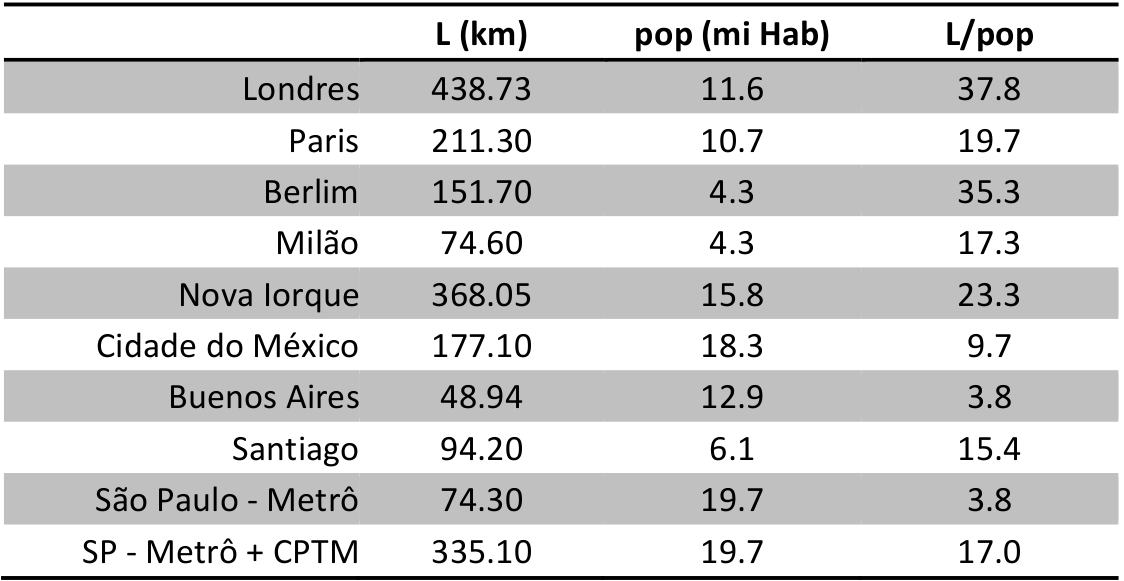
\includegraphics[keepaspectratio,width=\textwidth]{img_isoda_km_rede.png}
	\label{tab:isoda_km}
\end{table}

Assim como a criação da companhia, a operação de seis das sete linhas, nas quais todas exceto a 13-Jade são fruto de herança de estatais que pré-dataram a criação da {\glsdesc*{cptm}}, tem seu amparo por meio da Lei 7.861 de 1992, que retomo com o Art. 12:

\begin{citacao}
	Artigo 12 --- A \gls{cptm} deverá assumir os sistemas de trens urbanos da Região Metropolitana de São Paulo, operados pela Companhia Brasileira de Trens Urbanos - CBTU e pela Ferrovia Paulista S/A - FEPASA, de forma a assegurar a continuidade e a melhoria dos serviços, para isso podendo efetuar os necessários acordos operacionais.\\
	Parágrafo único --- Para o cumprimento do disposto neste artigo, a \gls{cptm} poderá celebrar contratos de prestação de serviços, gerenciamento de bens, ou quaisquer serviços de transporte de passageiros sobre trilhos ou guiados, de outras empresas ligadas ao sistema de transporte de passageiros na Região Metropolitana de São Paulo.\cite{lei7861}
\end{citacao}

Como explica \cite[pág. 30]{Isoda} em relação às redes conceituadas como metrô e surgidas em meados do século XIX, estas malhas ``Não se diferenciavam tecnológica e operacionalmente das estradas de ferro  existentes,  com  grande  número  de  ramais  e  trechos  de  via compartilhada. Eram linhas independentes, de companhias diversas, e muitas  vezes  buscavam  apenas  conectar  estações  terminais  centrais das ferrovias que não conseguiam penetrar nos centros antigos'', também segundo ele, é a partir daí que que os serviços suburbanos existentes começam a ser dinamizados em novas redes, que são ``impulsionadas  pela  necessidade  de  aumentar  o  rendimento  dos serviços  suburbanos  existentes.  As  principais  medidas  neste  sentido foram  a  segregação  das  linhas,  duplicando  o  número  de  vias  para separar serviços suburbanos dos serviços de longa distância e  cargas; construção  de  interligações  centrais,  em  túnel  ou  elevado, “amarrando” linhas que terminavam no centro; e construção de novas linhas. Estas medidas levam para a configuração de uma rede própria de trens urbanos de passageiros, tornando-a próxima de uma rede de metrô''\cite[pág. 32]{Isoda}.
	
\section{Evolução da demanda de passageiros}\label{ss:demanda}

Para \cite[p. 16]{Ferreira} a presença da \gls{cptm} é marcante no território, com resultados entusiasmantes após mais de uma década de investimentos, além disso, destaca que a \gls{cptm} serve 19 municípios na \gls{rmsp} (incluindo a capital paulista) e outros 3 fora dela (na \gls{auj}). Neste sentido, a presença da \gls{cptm} é sinônimo de presença do Trem Metropolitano, assim sendo, com base em \cite{Ferreira}[pág. 15, nota de rodapé 1], elaboro a seguinte tabela com os municípios atendidos:

\begin{center}
	\begin{longtable}{|l|l|l|}
		\caption{Cidades atendidas pela \gls{cptm} por linha} \\
		\hline
		\textbf{Linha} & \textbf{Município} & \textbf{Região} \\
		\hline
		\endfirsthead
		\multicolumn{3}{c}%
		{\tablename\ \thetable\ -- \textit{Continuado da página anterior}} \\
		\hline
		\textbf{Linha} & \textbf{Município} & \textbf{Região} \\
		\hline
		\endhead
		\hline \multicolumn{3}{r}{\textit{Continua na próxima página}} \\
		\endfoot
		\hline
		\endlastfoot
		Linha 7-Rubi & São Paulo & \gls{rmsp} \\
		Linha 7-Rubi & Caieiras & \gls{rmsp} \\
		Linha 7-Rubi & Franco da Rocha & \gls{rmsp} \\
		Linha 7-Rubi & Francisco Morato & \gls{rmsp} \\
		Linha 7-Rubi & Campo Limpo Paulista & \gls{auj} \\
		Linha 7-Rubi & Várzea Paulista & \gls{auj} \\
		Linha 7-Rubi & Jundiaí & \gls{auj} \\
		Linha 8-Diamante & São Paulo & \gls{rmsp} \\
		Linha 8-Diamante & Osasco & \gls{rmsp} \\
		Linha 8-Diamante & Carapicuíba & \gls{rmsp} \\
		Linha 8-Diamante & Barueri & \gls{rmsp} \\
		Linha 8-Diamante & Jandira & \gls{rmsp} \\
		Linha 8-Diamante & Itapevi & \gls{rmsp} \\
		Linha 9-Esmeralda & São Paulo & \gls{rmsp} \\
		Linha 9-Esmeralda & Osasco & \gls{rmsp} \\
		Linha 10-Turquesa & São Paulo & \gls{rmsp} \\
		Linha 10-Turquesa & São Caetano & \gls{rmsp} \\
		Linha 10-Turquesa & Santo André & \gls{rmsp} \\
		Linha 10-Turquesa & Mauá & \gls{rmsp} \\
		Linha 10-Turquesa & Ribeirão Pires & \gls{rmsp} \\
		Linha 10-Turquesa & Rio Grande da Serra & \gls{rmsp} \\
		Linha 11-Coral & São Paulo & \gls{rmsp} \\
		Linha 11-Coral & Ferraz de Vasconcelos & \gls{rmsp} \\
		Linha 11-Coral & Poá & \gls{rmsp} \\
		Linha 11-Coral & Suzano & \gls{rmsp} \\
		Linha 11-Coral & Mogi das Cruzes & \gls{rmsp} \\
		Linha 12-Safira & São Paulo & \gls{rmsp} \\
		Linha 12-Safira & Poá & \gls{rmsp} \\
		Linha 12-Safira & Itaquaquecetuba & \gls{rmsp} \\
		Linha 13-Jade & São Paulo & \gls{rmsp} \\
		Linha 13-Jade & Guarulhos & \gls{rmsp} \\
		\end{longtable}
\end{center}	

A \autoref{fig:demanda} apresenta um gráfico de demanda\footnote{Ver \gls{mdu}.} das seis linhas da empresa. Somadas, as linhas transportam mais de 2 milhões de passageiros. É oportuno salientar que a dissociação da rede da \gls{cptm} do território, acaba por eliminar um elemento estruturante importante, agravando o quadro de escassez de linhas por habitante, ao invés de induzir mudanças positivas, contudo, vale notar o papel difuso da \gls{cptm} apontado por \cite[p. 122]{Isoda}: 

\begin{citacao}
	(...) a \gls{cptm} tem hesitado em definir quais os seus papéis no transporte metropolitano, abarcando simultaneamente as escalas metropolitana, regional, e central-metropolitana (em grande parte por omissão da \gls{cmsp}).
\end{citacao}

\begin{figure}[h]
	\centering
	\caption{Gráfico de demanda baseado em \cite{sitecptm1} e \cite{sitecptm4}}
	\begin{tikzpicture}
	\begin{axis}[
	title=,
	grid=both,
	ymin=10,
	ymax=725,
	ybar,
	symbolic x coords={7,8,9,10,11,12,13},
	nodes near coords, nodes near coords align={vertical},
	xlabel=Linha,
	xtick=data,
	ylabel=Passageiros (MDU em milhares),
	enlargelimits=0.15,
	]
	\addplot+[ybar] coordinates
	{(7,450.100)
		(8,490.100)
		(9,601.300)
		(10,364.800)
		(11,724.400)
		(12,256.000)
		(13,13.489)};
	\end{axis}
	\end{tikzpicture}
	\label{fig:demanda}
\end{figure}

\section{Parceiras público-privadas em andamento}

\lipsum[3-4]

\section{Parceiras público-privadas fracassadas}

\lipsum[3-4]

\chapterimage{2019-02-09_est_passarela_l11} % Imagem do cabeçalho do capítulo
\chapter{O território atendido}

\section{Os municípios}

\lipsum[3-4]

\section{Potencialidades}

\lipsum[3-4]

\section{Eixos de desenvolvimento}

Sendo a malha da \gls{cptm} um elemento estruturante e gerida pelo governo estadual de São Paulo, apesar do enfraquecimento do papel do estado no planejamento do território, vale destacar que a mesma esfera de poder conta com uma estatal dedicada ao planejamento territorial da \gls{rmsp} e outras regiões metropolitanas, vide \cite[p. 224]{Stefani}, ``Cabe à \gls{emplasa} a execução de assessoramento ao Governo do Estado de São Paulo para questões metropolitanas. Nesse sentido, elabora projetos de uso e ocupação do solo, de urbanização e revitalização urbana, planos regionais e sub regionais, estudos sócio-econômicos e políticos. Presta ainda, assessoria técnica aos municípios do complexo metropolitano expandido: Grande São Paulo, Baixada Santista e Campinas, além das concentrações urbanas do Vale do Paraíba, Sorocaba e outras áreas de seu entorno''. Justifica-se, portanto, tal consideração quanto à presença de linhas da \gls{cptm}.

Apesar do papel institucional difuso da \gls{cptm} apontado por \cite{Isoda}\footnote{Vide menção na \autoref{ss:demanda}} e do atendimento herdado de outras estatais, \cite[pág. 97]{Ferreira} salienta que ``Como elemento para o planejamento e a organização da cidade, não parece haver dúvidas de que a \gls{cptm}, até agora, está credenciada a ter o papel indutor e estruturador que são creditados aos transportes de alta capacidade e de qualidade''. Os dois autores demonstram que problemas políticos e institucionais, bem como a conjuntura econômica de determinadas épocas, contribuíram para dificultar a segregação dos trens de carga e também avanços mais significativos no programa de modernização da \gls{cptm}. Tal condição não é surpreendente, visto que \cite[pág. 31]{Acselrad}, analisando as transformações de corte neoliberal, bem como outras ligadas à acumulação flexível, aponta: ``Tudo que diz respeito ao ordenamento	espacial regulamentar da cidade, inclusive suas dimensões ecológicas, se esvai em ausência	de forças de coordenação, que são eventualmente substituídas pela auto-organização da “governança corporativa”, da parceria privado-privado, ou seja, em parte crescente, pelos próprios capitais em competição''.

O Trem Metropolitano pode ser encarado como um elemento coesivo do território, no sentido infraestrutural, como elemento durável, referencial e articulador\footnote{``(\dots) os tempos dos retornos dos investimentos feitos na ferrovia são normalmente diferentes daqueles de outros investimentos e, principalmente, as suas características influem na localização das demais atividades humanas, modificam a paisagem de forma indelével, mesmo após seu abandono'' (\cite[pág. 13]{Ferreira})}.

Sendo a malha da \gls{cptm} um elemento estruturante e gerida pelo governo estadual de São Paulo, apesar do enfraquecimento do papel do estado no planejamento do território, vale destacar que a mesma esfera de poder conta com uma estatal dedicada ao planejamento territorial da \gls{rmsp} e outras regiões metropolitanas, vide \cite[p. 224]{Stefani}: 

\begin{citacao}
	(...) cabe à \gls{emplasa} a execução de assessoramento ao Governo do Estado de São Paulo para questões metropolitanas. Nesse sentido, elabora projetos de uso e ocupação do solo, de urbanização e revitalização urbana, planos regionais e sub regionais, estudos sócio-econômicos e políticos. Presta ainda, assessoria técnica aos municípios do complexo metropolitano expandido: Grande São Paulo, Baixada Santista e Campinas, além das concentrações urbanas do Vale do Paraíba, Sorocaba e outras áreas de seu entorno.
\end{citacao}

\section{Habitação social em complexos de habitação intensiva}

\lipsum[3-4]

\section{Situações em que a \gls{cptm} supera o Metrô}

Como costuma ser defendido em vários dos artigos publicados pelo COMMU, a Região Metropolitana de São Paulo tem hoje e cada vez mais, dois sistemas de metrô, um nascido pelas mãos do município e o outro, fruto da ``costura'' e de diferentes ferrovias, que continuam sendo modernizadas e transportando cada vez mais passageiros a cada ano. Décadas de desinvestimento e a passagem por uma série de periferias e cidades menos prestigiadas da metrópole, no entanto, colocam um dos sistemas no limbo. São listadas a seguir nove situações em que o ``patinho feio'' não é tão feio assim.

\subsection{Maior abrangência de atendimento, avançando por 22 municípios}

Como as linhas operadas pela \gls{cptm} nasceram pelas mãos de diferentes empresas ferroviárias, que operavam serviços em um contexto de atendimento totalmente diferente, ainda antes da fase de metropolização da Grande São Paulo, as 6 linhas acabam sendo mais abrangentes, com cerca de 130 km dentro da capital e 130 km fora da capital, com 92 estações ao todo. Os 130 km fora da capital percorrem 21 municípios, com o sistema funcionando em vários deles para deslocamentos internos, caso de Mogi das Cruzes (Jundiapeba, Braz Cubas, Mogi das Cruzes e Estudantes), Osasco (Presidente Altino, Osasco, Comandante Sampaio, Quitaúna e General Miguel Costa), Barueri (Antônio João, Barueri, Jardim Belval e Jardim Silveira) e Santo André (Utinga, Prefeito Saladino e Prefeito Celso Daniel-Santo André)

O atendimento a múltiplos municípios também permite um acesso conveniente a rodoviárias localizadas fora da capital, como os terminais rodoviários de Osasco, Santo André (Tersa) e Mogi das Cruzes (Geraldo Scavone), o que beneficia quem mora em diversas cidades atendidas pelas linhas da \gls{cptm}, além de moradores de certos bairros da capital, que não precisam se deslocar para estações como Portuguesa-Tietê, Palmeiras-Barra Funda e Jabaquara. Com a inauguração da Linha 13-Jade, o acesso ao terminal rodoviário de Guarulhos pela futura Estação Guarulhos-CECAP deverá beneficiar moradores do extremo leste da capital, de Poá e de Itaquaquecetuba. Como também veremos a seguir, o atendimento mais abrangente passa por uma série de centralidades (algumas delas fortes o suficiente para terem projeção metropolitana), sem deixar a região central da capital de lado (atendida pelas estações Brás, Júlio Prestes e Luz).

\subsection{Atendimento aos novos centros metropolitanos da capital}

O mérito quase acidental recai sobre a Linha 9-Esmeralda (Osasco-Grajaú), originada a partir de um tímido ramal da Estrada de Ferro Sorocabana, cujo atendimento de caráter urbano, ainda quando a metropolização da capital não tinha atingido seu auge, era extremamente precário e limitado. Décadas depois da ideia de implantar paradas como Monark (vizinha à fábrica de bicicletas homônima), a industrialização ao longo de uma das margens do Pinheiros passou a dividir espaço com o surgimento de edifícios de escritórios cada vez mais sofisticados, foi neste contexto, que no final da década de 1990 foi executado o programa de “dinamização da Linha Sul”, que concluiu estações previstas pela Fepasa, mas cujo poder público não havia tentado erguer, até aquele momento.

Os primeiros anos do novo milênio foram marcados pela inauguração de estações hoje já incorporadas à vida da capital, como Hebraica-Rebouças, Vila Olímpia, Berrini e Morumbi.

\subsection{Atendimento a importantes subcentros, inclusive fora da capital}

A herança diversa da \gls{cptm} se traduz num atendimento muito mais amplo, como comentado acima. Ainda que o atendimento possa ser qualificado como periférico (e até mesmo chamado de suburbano, embora as cercanias não costumem apresentar traços suburbanos, mas sim totalmente urbanos, ainda que nem sempre com infraestrutura adequada), ele também contempla centros com importância regional e metropolitana fora do município de São Paulo, tais localidades são relevantes para equilibrar a oferta de comércio e serviços, proporcionar algum grau de geração de empregos, além de abrigar órgãos do poder público. Em algumas situações o atendimento da \gls{cptm} pode funcionar como um sistema de alta capacidade aproximador, exigindo a utilização de uma linha de ônibus para atingir a centralidade.

\begin{itemize}
	\item Exemplos na Grande São Paulo:
		\begin{itemize}
			\item Mogi das Cruzes: atendimento ao centro histórico e comercial; atendimento ao centro cívico e Parque Monte Líbano, reduto gastronômico e boêmio do Alto Tietê;
			\item Suzano: a estação homônima atende um dos maiores centros de comércio popular do Alto Tietê, a região conhecida como Quadrilátero Central;
			\item Osasco: a área composta pelo calçadão de Osasco (atendida pela estação que leva o nome da cidade) e seu entorno é uma das mais dinâmicas quando se fala em comércio popular no oeste da Grande São Paulo, na verdade, ela é tão dinâmica, que só perde em volume de consumidores para a 25 de Março, na capital;
			\item Barueri (Alphaville): diversas empresas instalaram seus escritórios em Alphaville devido ao baixo ISS, o que por sua vez fortaleceu a instalação de centros comerciais e o surgimento de um centro metropolitano que rivaliza com a Berrini, na capital; as estações Barueri, Antônio João e General Miguel Costa fornecem os acessos mais cômodos no ponto de vista da intermodalidade (Trem Metropolitano-ônibus intermunicipal e Trem Metropolitano-ônibus municipal);
			\item Santo André: além do comércio popular presente no calçadão Oliveira Lima, cujo charme recai ao trecho coberto, a cidade abriga indústrias e um polo gastronômico no Bairro Jardim; o complexo formado pela Estação Prefeito Celso Daniel-Santo André e os terminais \gls{emtu} Santo André Leste e Santo André Oeste impressiona, permitindo também acesso ao Corredor ABD;
			\item São Caetano do Sul: o IDH elevado da pequena cidade, cujo sistema de ônibus conta com apenas 8 linhas, é reforçado por bairros simpáticos como o Barcelona (Estação Utinga) e uma região central bem integrada à \gls{cptm} (Estação São Caetano).
		\end{itemize}
	\item Exemplos em São Paulo:
		\begin{itemize}
			\item Lapa: o bairro é atendido por duas estações com seu nome, possuindo um tradicional mercado municipal, terminal de ônibus (conectado à Estação Lapa da Linha 8-Diamante por um calçadão arborizado) e forte comércio popular (conectado à Estação Lapa da Linha 7-Rubi por uma passagem subterrânea);
			\item São Miguel Paulista: nas proximidades da antiga estação diversas ruas foram convertidas em calçadão, abrigando intenso comércio popular. A atual estação está localizada a poucos metros da antiga e o acesso principal fica de frente para a Praça do Forró e a Capela de São Miguel Arcanjo; sua força como centralidade fica reforçada por ligações perimetrais da \gls{sptrans} para a Estação Guaianazes, além de linhas de ônibus com destino à periferia de Guarulhos;
			\item Itaim Bibi: estações como Vila Olímpia e Cidade Jardim permitem acesso a um conjunto impressionante de escritórios e “ecossistema” de apoio, como bares, restaurantes e shopping centers; enquanto a Estação Cidade Jardim permite acessar o Parque do Povo, a Estação Vila Olímpia possui acesso para a Ciclovia Rio Pinheiros.
		\end{itemize}
\end{itemize}

\subsection{Pioneirismo na utilização de trens com ar condicionado}

\begin{wrapfigure}{l}{0.5\textwidth}
	\centering
	\caption[QR Code para vídeo do Expresso Leste em 1998]{QR Code para vídeo de uma visita programada no Expresso Leste, dois anos antes de sua inauguração. O trem usado naquele dia, da série 2100, já contava com ar condicionado, algo que a Zona Leste só conheceria pelas mãos da \gls{cmsp} no longínquo ano de 2010}
	\qrcode[version=1,height=4cm]{https://www.youtube.com/watch?v=IpU47P2R1rw}
	\label{qr:video_1998_l11}
\end{wrapfigure}

Os primeiros trens com ar condicionado da \gls{cptm} chegaram em 1998, sendo um marco notável a inauguração do Expresso Leste em 27/05/2000, o qual contou com uma frota de trens inteiramente nova e dedicada para o novo serviço expresso, que naquela altura operava entre as estações Brás e Guaianazes (esta última contando com um edifício inteiramente novo em relação ao que era usado anteriormente).

A \glsdesc{cmsp} (geralmente chamada de Metrô) ganhou seus primeiros trens com ar condicionado na Linha 5-Lilás, inaugurada em 2002, porém, a linha foi construída pela \gls{cptm} e a especificação do salão dos trens seguiu praticamente o paradigma adotado por ela para a malha do Trem Metropolitano, daí a presença de ar condicionado, bancos com revestimento de tecido e portas entre carros. O Metrô só receberia trens com ar condicionado especificado conforme suas diretrizes em 2006, um atraso de aproximadamente 8 anos em relação à Companhia Paulista de Trens Metropolitanos, porém, enquanto o Expresso Leste iniciou do zero com trens refrigerados, a Linha 3-Vermelha, sua “prima” paradora, precisou esperar até 2010, ano de estreia da Frota H.

\subsection{Oferta de bicicletários}

Sem dúvida a \gls{cptm} está na frente quando falamos em operar e construir bicicletários. Os motivos são claros: eles estão em maior número, estão espalhados tanto em estações periféricas quanto em estações-chave da RMSP, são maiores e, finalmente, possuem um horário de funcionamento muito mais confortável. Enquanto os bicicletários da \gls{cptm} funcionam no mesmo horário de referência das estações, ou seja, dom-sex das 4h00 à 0h00 e sábados das 4h00 à 1h00, cobrindo basicamente todo o horário de funcionamento das 6 linhas da estatal, a Companhia do Metropolitano insiste em operar seus poucos bicicletários seg-seg das 6h00 às 22h00. Duas estações da \gls{cptm} integradas a parques do Governo do Estado de São Paulo possuem bicicletário: Villa Lobos-Jaguaré (233 vagas) e Engenheiro Goulart (152 vagas).

Os maiores bicicletários da \gls{cptm} contam com 576 e 480 vagas, localizados respectivamente nas estações Suzano e Itapevi. A capacidade dos bicicletários da Companhia do Metropolitano foi alvo de crítica pelo Mobilize em 2016. Há uma exceção para os bicicletários das estações Pinheiros (que também é uma estação da \gls{cptm}, na Linha 9) e Fradique Coutinho, operados pela concessionária ViaQuatro: eles seguem a mesma lógica de horários da \gls{cptm}, porém análoga ao horário do sistema da Companhia do Metropolitano, ficando abertos dom-sex das 4h40 à 0h00 e sábados das 4h40 à 1h00.

\subsection{Paralelismo em alguns trajetos}

O passado das antigas ferrovias favorecem a \gls{cptm} e quase chega a ser uma covardia comparar, no entanto, como o sistema da Companhia do Metropolitano é bem mais recente e não precisou de um processo intenso de modernização (uma verdadeira reconstrução, dependendo do caso), não há qualquer razão para ignorar fatos. A estrutura do trecho Tatuapé-Lapa possibilita uma série de estratégias em situações específicas (como greves), além de garantir algum grau de paralelismo. Chegamos a destacar características do trecho em nosso artigo sobre o tema "metrô 24 horas", não deixe de conferi-lo.

Por exemplo, partindo da Estação Tatuapé, é possível chegar na Estação Brás com as linhas 11-Coral (Luz-Guaianazes-Estudantes) e 12-Safira (Brás-Calmon Viana), ainda, a Estação Barra Funda pode ser acessada diretamente da zona central por meio de duas estações: Luz e Júlio Prestes, usando as linhas 7-Rubi (Luz-Francisco Morato-Jundiaí) e 8-Diamante (Júlio Prestes-Itapevi-Amador Bueno), respectivamente. Adicionalmente, a presença de duas estações Lapa, com as linhas 7 e 8 correndo paralelas até aquela altura, adiciona mais um exemplo de paralelismo.

Já em relação às situações específicas, é relativamente comum observar a operação da Linha 7-Rubi até a Estação Brás, a estratégia é colocada em prática durante greves e ações de manutenção/modernização. Também já houve registro de uma operação especial para torcedores do Palmeiras, na qual o Expresso Leste ofertou uma viagem a partir da Estação Palmeiras-Barra Funda (paralelismo com a Linha 7-Rubi até a Luz, portanto).

\subsection{Pioneirismo na adoção de bilhetes com QR Codes}

Aparentemente a \gls{cptm} tem desejado reduzir o uso do bilhete magnético, para tanto, mapeou as estações nas quais ele era mais usado e propôs uma alternativa em parceria com a Autopass (a mesma do Cartão BOM, utilizado nos intermunicipais da \gls{emtu}): emitir a passagem com \textit{QR Codes} impressos (vide \autoref{fig:l8_qr}).

\begin{figure}[b!]
	\centering
	\caption[Informativo QR Codes]{Folheto explicativo distribuído na Estação Lapa da Linha 8-Diamante}
	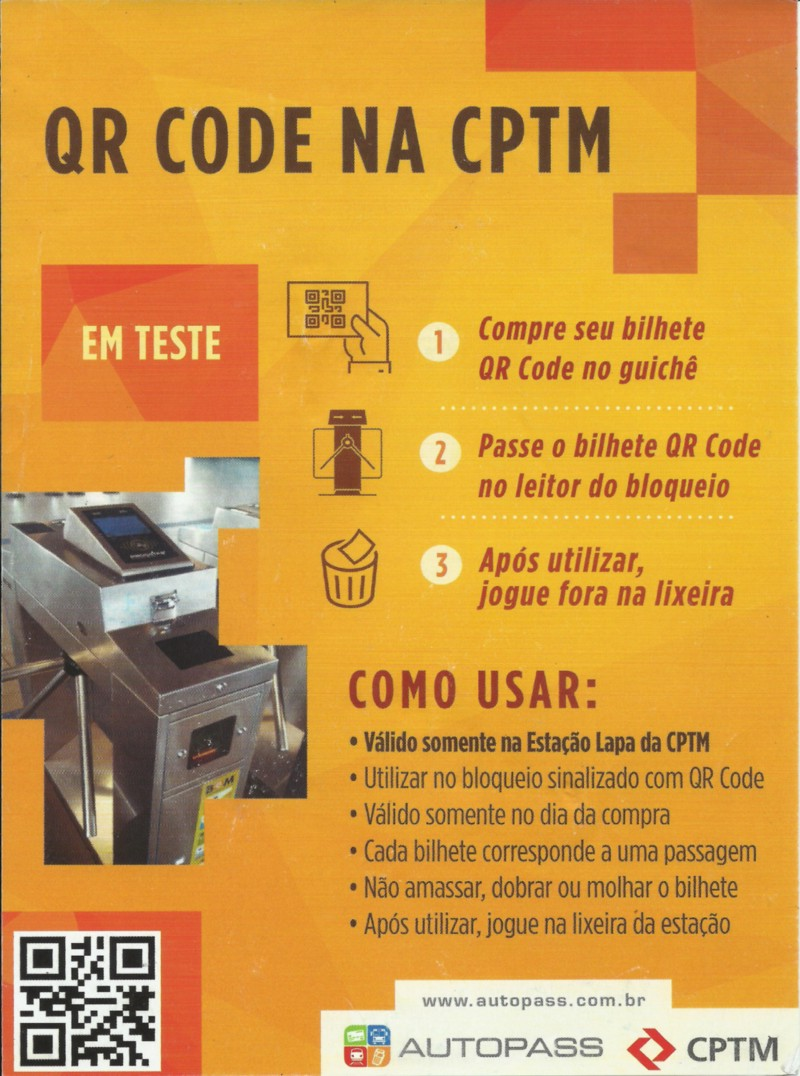
\includegraphics[width=\linewidth]{informativo_l8_qrcode}
	\label{fig:l8_qr}
\end{figure}

Para ter uma ideia da quantidade de QR Codes gerados e quais as estações participantes, confira fragmento de uma notícia oficial do início de 2017:

\begin{citacao}
	Entre outubro e dezembro do ano passado, foram emitidos mais de 61 mil bilhetes com QR Code nas seguintes estações: Vila Aurora, na Linha 7-Rubi, Lapa, na Linha 8-Diamante, Autódromo, na Linha 9-Esmeralda, Tamanduateí, na Linha 10-Turquesa, Dom Bosco, na Linha 11-Coral, e USP Leste, na Linha 12-Safira. (\cite{sitecptm_vendaqr})
\end{citacao}

A iniciativa repercutiu até em sites como o Tecnoblog\footnote{Ver \cite{higa2017}}.

\subsection{Sustentabilidade pioneira na Estação USP Leste}

Poucos anos depois de sua inauguração, há cerca de sete anos, uma reportagem do Estadão apontava que a estação foi a primeira sustentável do mundo, posicionamento reiterado pelo portal AECweb em 2011

%TODO fotos de USP Leste

Não ficou claro se a certificação foi de fato obtida, mas é inegável que houve uma tentativa e que até a pintura que revestia a cobertura da plataforma foi trocada.

\subsection{Denúncias por SMS e pianos nas estações}

---

Talvez você não se lembre, mas conforme uma antiga notícia do portal do Governo do Estado de São Paulo\footnote{\url{http://www.saopaulo.sp.gov.br/spnoticias/ultimas-noticias/piano-da-estacao-da-luz-faz-sucesso-com-o-publico/}}, a ideia de colocar dois pianos à disposição dos passageiros começou em 2009:

\begin{citacao}
	Em 2009, o Sesc doou os dois pianos da marca Zimmermann para a \gls{cptm}. O projeto deveria durar apenas algumas semanas, mas os pianos caíram no gosto do público e devem ficar por tempo indeterminado. Tal é o sucesso do Toque-me, sou teu, que a \gls{cptm} produziu o CD - Piano na Luz como parte da comemoração por seus 17 anos em junho de 2009. Participaram do disco as sete pessoas que mais se destacaram em suas apresentações espontâneas.
\end{citacao}

Após alguns anos, o programa infelizmente terminou, sendo que o último piano a passar pela \gls{cptm} foi na ocasião do 462º aniversário de Santo André, no Grande ABC. No Metrô, o programa, que também já terminou, surgiu em março de 2011 (conforme informações de uma antiga notícia da Companhia do Metropolitano), ou seja, surgiu dois anos depois de ser iniciado com sucesso na \gls{cptm}.

Já no caso do SMS Denúncia, o espaço entre a implantação na \gls{cptm} e no Metrô foi ainda maior: enquanto o passageiro do Trem Metropolitano passou a contar com o serviço em novembro de 2008, conforme informações do site oficial da \gls{cptm}, o passageiro do Metropolitano de São Paulo ganhou a mesma possibilidade apenas em janeiro de 2011, também conforme uma antiga notícia, ou seja, cerca de três anos depois.

\begin{info}
	\infocaio{26/08/2017}{https://goo.gl/3EYVrT}
\end{info}

%----------------------------------------------------------------------------------------
% 	PARTE 2
%----------------------------------------------------------------------------------------

\part{Análise}

\chapterimage{2019-02-09_ego_sinal68} % Imagem do cabeçalho do capítulo
\chapter{Apropriando-se da infraestrutura}

\section{Cerca de 130 km de trilhos esquecidos dentro da capital}

A rede da \gls{cptm}, com cerca de 272 km, atendendo 23 municípios, com mais de 90 estações, aproximadamente 170 trens e movimentação de quase 3 milhões de usuários em média por dia útil apresenta não só números superlativos, mas também descaso em igual ou superior escala. A capital possui cerca de 130 km (136,5 km em 2014, para ser mais exato, de acordo com a Secretaria dos Transportes Metropolitanos\footnote{\url{http://www.stm.sp.gov.br/index.php/obras/modernizacao/modernizacao-na-cptm}}), o que é mais do que a rede do Metrô inteira, mesmo se somarmos a Linha 4, operada pela CCR ViaQuatro em regime de concessão patrocinada).

Mesmo com mais de 100 km dentro da capital, mesmo atendendo a espécie de “centro nervoso” que se tornou a região da Marginal Pinheiros, mesmo interligando o ABC e a capital, mesmo atendendo à Zona Leste com o único serviço expresso sobre trilhos de toda malha, continua sendo tratada como cidadã de segunda classe. E o pior: o tratamento questionável está por todos os lados, de utilizadores a jornalistas e até supostos especialistas, contaminando o viés político que qualquer obra de infraestrutura feita por um órgão estatal carrega por natureza. Enquanto os holofotes se voltam apenas ao Metrô, a requalificação da malha da \gls{cptm}, que já chegou a prever trens de quatro carros e intervalos (na época) teoricamente baixos, continua se arrastando a medida que a demanda não para de aumentar, com um modelo operacional que parece ter se adaptado às pressas a uma realidade que não havia sido prevista, para variar, subestimou-se os subúrbios e sua demanda de passageiros, talvez isso explique o sepultamento do Projeto Integração Centro (projeto este comentado na \autoref{ss:icentro}).

O corredor do Integração Centro na Estação Luz saturou, a integração na Estação Santo Amaro continua sendo motivo de estresse para usuários das linhas 5-Lilás e 9-Esmeralda (originalmente se previa a conexão em uma outra estação, chamada de João Dias, que apesar de perder a intermodalidade, vez ou outra é citada pela imprensa), a ingerência em relação a obras de infraestrutura e contratos de prestação de serviços atingiu níveis críticos, reduzindo a confiabilidade do sistema, fazendo com que os novos trens revelassem a falta de capacidade administrativa da \gls{cptm} em se modernizar sem abandonar as próprias raízes. Nada disso, porém, parece despertar fortemente o interesse da chamada “grande mídia”, aquela que ataca apenas os sintomas do transporte público ao passo que anúncios de carros 1.0 com prestações a perder de vista são convenientemente vomitados nas telas e páginas. Mesmo nas denúncias de cartel o enfoque continua sendo dado ao Metrô, sendo que contratos de manutenção de pelo menos três séries de trens da \gls{cptm} fazem parte do escândalo.

De acordo com o jornal Folha de S.Paulo, os intervalos de 3 minutos são prometidos desde o governo Fleury, é o que revela trecho de matéria publicado em 15 de setembro de 1991 (a edição em questão pode ser buscada no acervo), na época, o governador em questão já prometia intervalos de 3 minutos e a mesma qualidade do Metrô para o transporte suburbano, no mesmo parágrafo, a declaração do governador fazia parecer que os intervalos eram de 8 minutos, o que estava longe de ser verdade para as linhas Tronco e Variante, atuais 11-Coral e 12-Safira, por exemplo, que apresentavam um intervalo praticamente dobrado em relação ao declarado. Os mesmos intervalos são prometidos até os dias atuais, no portal G1, em matéria do dia 11 de abril de 2013, o mesmo intervalo foi prometido, ironicamente e, assim como na Folha de 1991, o leitor foi induzido a erro, pois nem todas as linhas da \gls{cptm} operam com 5 minutos de intervalo no horário de pico, também não foi implementado, até os dias atuais, uma forma de acompanhamento dos intervalos, com os horários entre uma e outra composição, item primordial a meu ver.

Enquanto a imprensa alimenta inconsequentemente comparações infundadas com sistemas de metropolitano centenários, pelo menos parcialmente construídos ao custo de muita mão de obra trabalhando em condições sub-humanas e inseridos em um contexto econômico, social e urbanístico totalmente distintos em relação ao cenário paulista, a mesma imprensa também comete gafes imperdoáveis ao considerar sistemas de metrô comparáveis a \gls{cptm} em termos de intervalo, com padrão de serviço inferior ou similar, ao mesmo tempo que parece desclassificar ou não enxergar a \gls{cptm}. Ademais, as requalificações feitas no trecho Mauá-Pirituba da então Estrada de Ferro Santos-Jundiaí são sempre ignoradas (atualmente o trecho é das linhas 10-Turquesa e 7-Rubi), bem como a modernização dos serviços de subúrbio da Fepasa nas linhas Oeste (atual 8-Diamante) e Sul (9-Esmeralda), o que só enfraquece uma análise mais coesa sobre a situação de toda a rede de trilhos, mesmo no antigo sistema Leste (linhas Tronco e Variante), estações foram reconstruídas (é o caso de Suzano, Ferraz de Vasconcelos, Mogi das Cruzes, da antiga São Miguel Paulista etc), para não dizer que o processo de chegada do próprio Metrô à Zona Leste remete a diversas questões, inclusive ao fato de que \textbf{a região de Itaquera não recebeu os devidos cuidados previstos}, tese esta\footnote{\url{http://www.teses.usp.br/teses/disponiveis/102/102132/tde-26042013-105748/pt-br.php}} que é uma leitura recomendada para quem quiser entender mais um pouco sobre a delicada questão da Linha 3-Vermelha, vale lembrar, outrossim, que a chegada da Linha 3 causou alterações no viário (a Radial Leste fala por si só), mudanças nos ônibus (nunca a Zona Leste recebeu tantos terminais de ônibus) e, principalmente: aproveitou parte da faixa de domínio da Linha Tronco, algo que até os dias atuais provoca contraste, positivo e negativo, entre a Linha 3 e os trens do Expresso Leste da Linha 11-Coral da \gls{cptm}.

\subsection{Requalificação é elemento-chave}

A verdadeira requalificação da \gls{cptm} é de fundamental importância para uma possibilidade de melhorar substancial a vida de, pelo menos, uma parcela significativa que vive na metrópole, mesmo que apenas a trabalho.

O projeto do expresso\footnote{\url{http://www.agenciainterativa.com.br/clientes/aspea/ver_materia.asp?id=698}} entre a sub-região Oeste da Região Metropolitana e a Zona Oeste da cidade de São Paulo, alterando a vida de quem utiliza as linhas 8 e 9, por exemplo, é muito pouco discutido, nele, um trem expresso com paradas nas estações Barueri, Carapicuíba e Osasco vai direto para a Estação Pinheiros, terminal do serviço. O projeto também esbarra com outra mudança: a da Linha 9 passar fazer terminal na Lapa, se conectando às linhas 7 e 8, algo que remete assim como o próprio Expresso Oeste-Sul ao ano de 2011.

\begin{figure}[!htb]
	\caption[Diagrama do Expresso Oeste-Sul]{Infográfico sobre o Expresso Oeste-Sul, extraído do link da ASPEA no parágrafo acima}
	\centering
	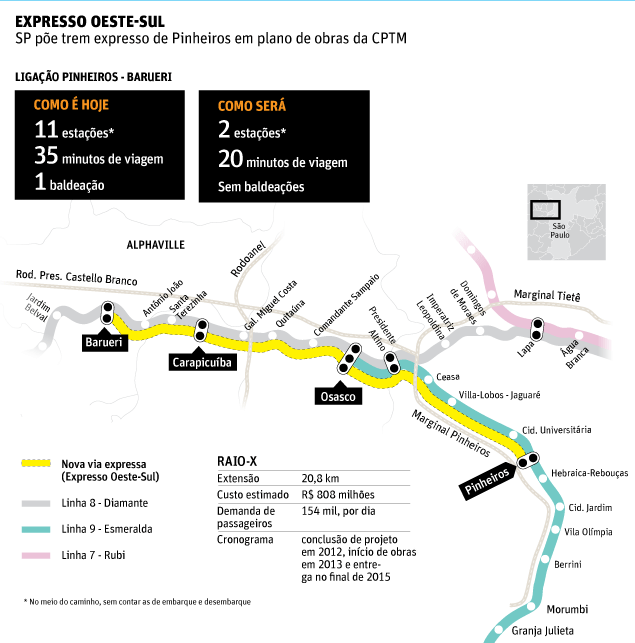
\includegraphics[width=\linewidth]{aspea_oeste-sul}
	\label{fig:aspea_oeste-sul}
\end{figure}

Outra mudança que foi anunciada e que caiu rapidamente no esquecimento foi aquela voltada ao saturado corredor da Estação da Luz, não só nada mais se falou com relação a aberturas de mais saídas e de uma conexão com a subutilizada Estação Júlio Prestes da Linha 8, como também não se observou qualquer esboço por parte da \gls{cptm} de, pelo menos, remover os esqueletos das antigas lojas de conveniência que existiam em parte da área subterrânea, o jovem corredor de integração, hoje com apenas dez anos de idade, assim como a Linha 9, se viu em situação ainda mais complicada assim que a Linha 4 começou a ganhar popularidade. Aqueles que conhecem a integração da Linha 4 na Estação Luz nos horários de pico provavelmente entendem muito bem o significado da palavra gambiarra; não se optou por alargar a galeria e confeccionar uma integração digna, que resgatasse a elegância do comércio que existia, facilitasse a integração e acomodasse melhor o fluxo de passageiros oriundo não somente da realidade atual, mas também de, pelo menos, mais duas ou três décadas, apenas se criou uma abertura e um redirecionamento de fluxo bruto e inconveniente.

\begin{wrapfigure}{l}{0.5\textwidth}
	\centering
	\caption[QR Code com renders do eixo Lapa-Brás pela Fupam]{QR Code com o link da segunda revisão do vídeo a respeito do projeto da Fupam para a \gls{cptm}, contemplando o eixo Lapa-Brás}
	\qrcode[version=1,height=4cm]{https://www.youtube.com/watch?v=DHIgwpfMiy0}
	\label{qr:video_fupam}
\end{wrapfigure}

Um projeto maior e que teoricamente permite a eliminação de gargalos operacionais históricos é aquele da Fupam. O projeto da Fupam leva o nome de Tronco Metropolitano da Mobilidade Urbana, dando um tom de vida própria ao trecho dentro da abrangência do projeto, em que as linhas são vistas como articuladoras importantes, não meras alimentadoras do Metrô. O projeto escrito pode ser conferido aqui, ao passo que o vídeo mais recente pode ser conferido abaixo:

O projeto da Fupam, ainda que não totalmente maduro, é interessante por explorar um dos eixos mais cruciais de parte da rede da \gls{cptm}, que vai do Brás até a Lapa, identificando pontos de interesse e/ou de relevância ao longo do trajeto, a medida que intervenções urbanas no entorno imediato se desdobram, ou seja, é um projeto que viabiliza uma requalificação urbana talvez comparável com as obras realizadas pela França na então inédita RER (Rede Expressa Regional), com estações subterrâneas estratégicas em Paris, alterando a experiência de utilização dos serviços de subúrbios, o emprego de uma perfuratriz e a modernidade e sofisticação do sistema marcaram uma matéria da revista Popular Science a respeito, datada de agosto de 1972\footnote{\url{encurtar.com}}. O projeto prevê a existência de cargueiros e é provavelmente uma das propostas mais arrojadas feitas até o momento para a requalificação da \gls{cptm}. Humildemente, especulo que levar a Linha 11 até a Estação Lapa poderia mudar o cenário da Estação República e também ajudar a fortalecer ainda mais o tronco proposto, eu diria que as possibilidades são tamanhas, de maneira que é possível repensar também a questão da Linha 12-Safira, hoje confinada na Estação Brás, além da Linha 13-Jade, que vem ganhando certa notoriedade em vista do andamento das obras, acredito que a conexão em Brás, provavelmente uma das piores em todo o sistema poderia ter seu uso completamente alterado, o que beneficiaria diretamente a Linha 3, hoje o Brás é sem dúvida alguma uma das paradas mais críticas da linha, quando os trens já abarrotados têm os passageiros colocados a prova, sendo várias as cenas de desrespeito no embarque.

\subsection{Extrapolando o termo ``metrô'': urbano e regional}

Inserido nas entrelinhas do presente texto, o termo ``metrô'' ainda causa confusão entre algumas pessoas. Na Revista Engenharia 607, o especialista Peter Alouche fala de metrô regional e metrô urbano e, ainda que as características possam se confundir em diversos momentos, é uma maneira muito mais simples de tratar o transporte pesado sobre trilhos em São Paulo. O trecho relevante do artigo do Peter pode ser conferido aqui, na página 107, segundo ele, a \gls{cptm} é um sistema de metrô regional, o que faz absolutamente sentido, é sinônimo também do termo “metrô regional” um que vem caindo em desuso, inclusive pela própria \gls{cptm}: “trem metropolitano”, são duas palavras que consagraram a modernização promovida pela Fepasa e a \gls{cptm} é a Companhia Paulista de Trens Metropolitanos.

\subsection{Conclusão}

Como tentei mostrar, ao limitarmos virtualmente o campo de atuação de um sistema de transporte, limitamos também sua importância, não só em termos políticos, mas também sociais. A requalificação e modernização definitiva da \gls{cptm} inclui mais do que máquinas e procedimentos operacionais, ela está ligada intrinsecamente ao aspecto humano, relacionado aos empregados e também aos usuários. Acelerar o processo depende fortemente da forma como o sistema é percebido, podemos estar a perder uma grande oportunidade e quando nos dermos conta, os custos e as dificuldades poderão ser ainda maiores.

\begin{info}
	\infocaio{24/10/2014}{https://goo.gl/i7aVkT}
\end{info}

\section{Estação Luz}\label{s:luz}\index{Estação Luz}

Imponente por fora, a estação vive hoje cenas de saturação, que muitas vezes levam a comportamentos no mínimo duvidosos (para não dizer arriscados) nos horários de pico. A estrutura, de arquitetura inglesa, revela uma rotina apressada, que por vezes sobrepõe-se a razão. A Estação da Luz merece viver melhores dias e, com ela, todos os passageiros e passageiras.

\subsection{Projeto Integração Centro}\label{ss:icentro}\index{Integração Centro}

Oficialmente, a \gls{cptm} informa como data de inauguração a data de 30/11/2004, a informação está contida na área de linhas do site\footnote{\url{https://www.cptm.sp.gov.br/sua-viagem/Pages/Linhas.aspx}}. O ano de 2004 está relacionado com o fracassado Projeto Integração Centro, uma tentativa de conexão entre as seis linhas da \gls{cptm} e o eixo central (Brás-Luz-Barra Funda), que na altura acabou subestimando a demanda dos subúrbios e o próprio papel do sistema de trilhos, que passava a ganhar contornos de malha integrada, algo que até então ainda não era tão enfatizado.

Pagamos o preço pelas limitações oriundas do Integração Centro até os dias atuais. Corredores e acessos foram dimensionados para um universo em que o intervalo era de 10 minutos e a demanda das linhas da \gls{cptm} não chegava nem perto dos cerca de 3 milhões atuais. Projetos ruins no passado significam sofrimento por até uma década ou mais.

Mesmo com as limitações, é preciso mencionar que o projeto foi o responsável pelo corredor de integração entre a \gls{cptm} e o Metrô, indispensável nos dias atuais. Na época a estação também foi reformada e ao passar a contar com acessos subterrâneos, teve a plataforma central remodelada e ganhou novos sanitários.

\subsection{Transformações recentes}

Nos últimos 15 anos, a estação sofreu mudanças quanto às linhas disponíveis para embarque a partir dela. Abaixo podemos conferir quais linhas operam atualmente.

\begin{center}
	\begin{longtable}{|l|l|l|}
		\caption{Linhas que operam na Estação Luz} \\
		\hline
		\textbf{Linha} & \textbf{Responsável} & \textbf{Caráter} \\
		\hline
		\endfirsthead
		\multicolumn{3}{c}%
		{\tablename\ \thetable\ -- \textit{Continuado da página anterior}} \\
		\hline
		\textbf{Linha} & \textbf{Responsável} & \textbf{Caráter} \\
		\hline
		\endhead
		\hline \multicolumn{3}{r}{\textit{Continua na próxima página}} \\
		\endfoot
		\hline
		\endlastfoot
		1-Azul & \gls{cmsp} & Estatal \\
		4-Amarela & \gls{cmsp} & Concessão patrocinada à iniciativa privada \\
		7-Rubi & \gls{cptm} & Estatal com serviços concedidos à iniciativa privada \\
		11-Coral & \gls{cptm} & Estatal com serviços concedidos à iniciativa privada \\
	\end{longtable}
\end{center}

Com a chegada da Linha 4-Amarela, o corredor de integração foi modificado, passando a contar com um novo acesso na lateral. Uma espécie de “desvio” foi feito na tentativa de organizar o fluxo nos horários de pico e a impressão de “puxadão” é inevitável. A integração, já saturada, ganhou ares de improviso.

Outro aspecto notável é que depois da chegada da Linha 4, a Linha 10 foi retirada da estação, passando a fazer terminal na Estação Brás. A operação das linhas 7 e 10 sempre foi ruim e, na verdade, a gare histórica de 1901 não foi pensada como terminal.

Simplesmente faltava uma plataforma adicional para viabilizar a operação que a \gls{cptm} tentava fazer. Como a operação era feita numa única plataforma para as linhas 7 e 10, chegou-se ao limite de maneira relativamente rápida e os seguintes fatores inviabilizadores surgiram:

\begin{itemize}
	\item Demanda crescente nas linhas da \gls{cptm};
	\item Dificuldade de esvaziamento da plataforma central;
	\item Redução de intervalos nas linhas da \gls{cptm};
	\item Chegada da Linha 4.
\end{itemize}

A \gls{cptm} decidiu, mesmo após realização de obras na via permanente, manter a Linha 10 no Brás. A decisão revoltou alguns passageiros e contrariou o informativo impresso que chegou a ser distribuído na época, como podemos ver na \autoref{fig:l10_luz}.

Se observarmos os dados de demanda atuais fornecidos pela \gls{cptm} e apresentados na \autoref{ss:demanda} por meio da \autoref{fig:demanda}, temos o seguinte quadro: entre as três linhas da \gls{cptm} que utilizavam a Estação Luz, a Linha 10 segue sendo a de menor demanda em média por dia útil.

\begin{figure}[!htb]
	\centering
	\caption{Gráfico de demanda baseado em \cite{sitecptm1} e no gráfico utilizado no artigo original que deu origem a esta seção, veja \textit{infobox} ao final}
	\begin{tikzpicture}
	\begin{axis}[
	title=,
	grid=both,
	ymin=10,
	ymax=725,
	ybar,
	symbolic x coords={7 (2014), 7 (2019), 10 (2014), 10 (2019), 11 (2014), 11 (2019)},
	nodes near coords, nodes near coords align={vertical},
	xlabel=Linha (ano),
	xtick=data,
	x tick label style = {font = \small, text width = 1.7cm, align = center, rotate = 70, anchor = north east},
	ylabel=Passageiros (MDU em milhares),
	enlargelimits=0.15,
	]
	\addplot+[ybar] coordinates
	{(7 (2014),468.000)
		(7 (2019),450.100)
		(10 (2014),355.600)
		(10 (2019),364.800)
		(11 (2014),701.200)
		(11 (2019),724.400)};
	\end{axis}
	\end{tikzpicture}
	\label{fig:demanda}
\end{figure}

\begin{landscape}
	\begin{figure}[h]
		\centering
		\caption[Mapa do Integração Centro]{Antigo mapa do transporte metropolitano, com o Integração Centro em destaque}
		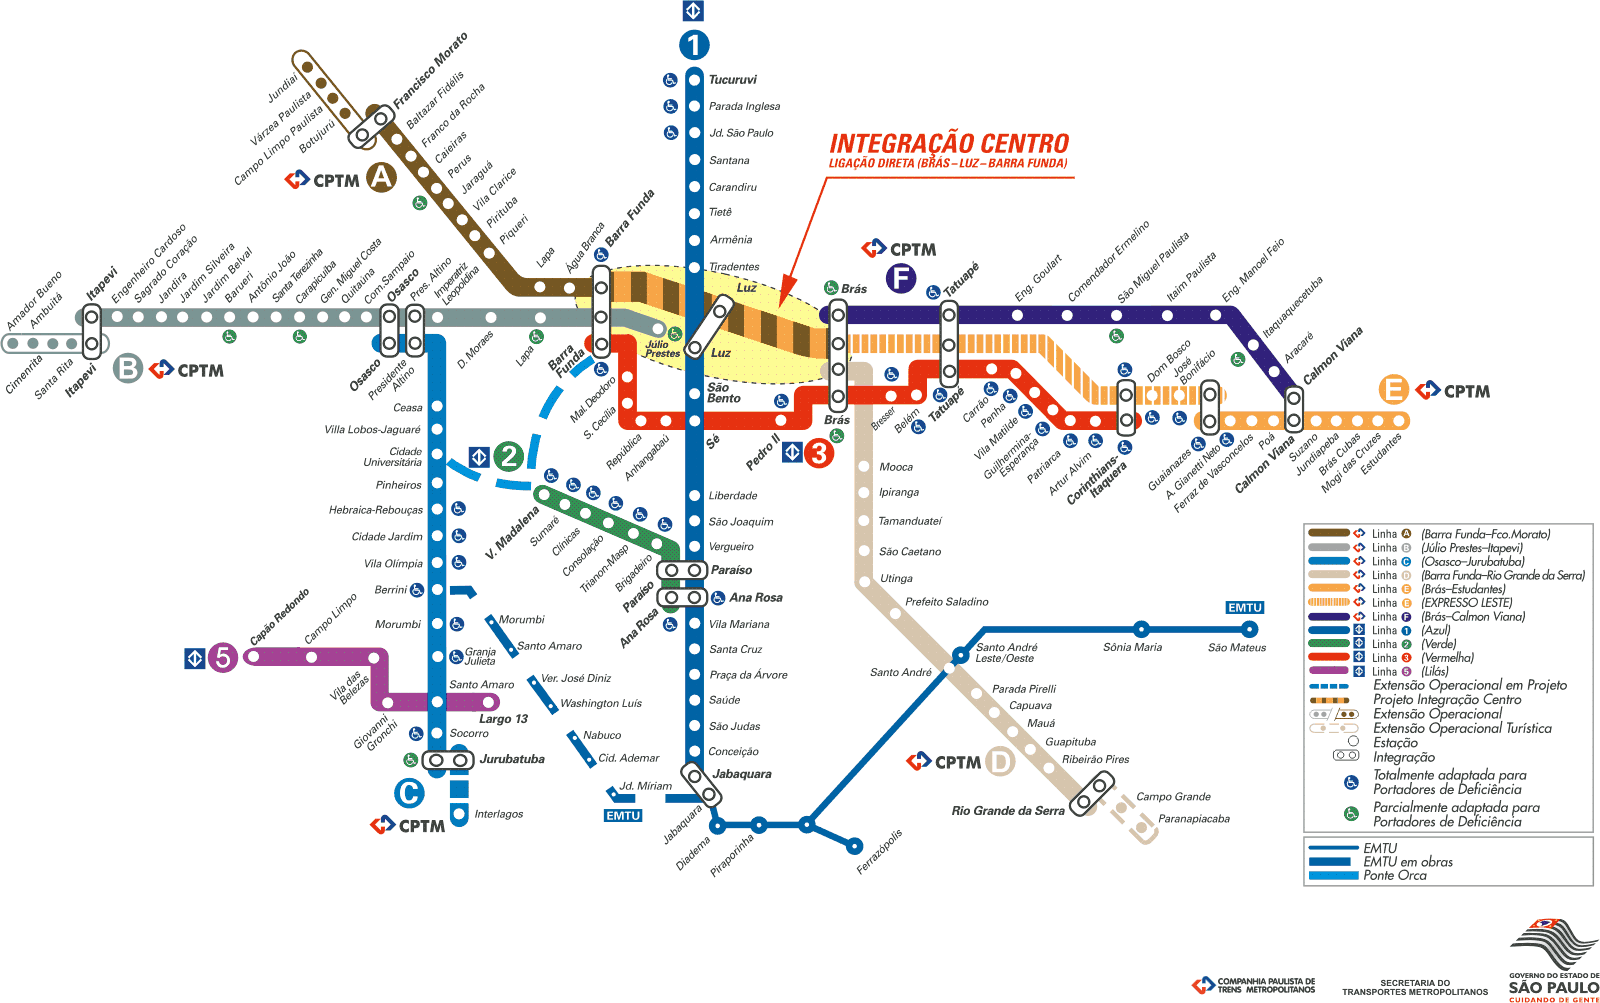
\includegraphics[width=21cm]{diagrama_integracao_centro}
		\label{fig:diag_ic}
	\end{figure}
\end{landscape}


\begin{figure}[tp]
	\caption[Informativo agosto/2011]{Informativo distribuído em agosto de 2011}
	\centering
	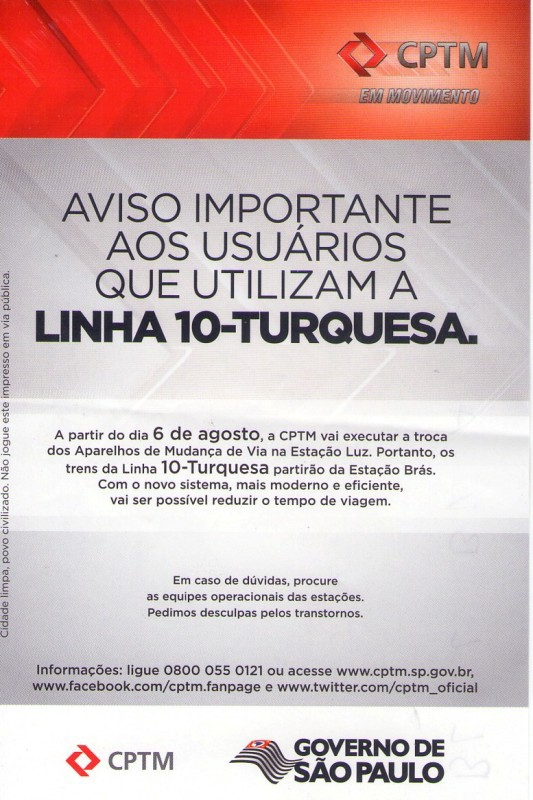
\includegraphics[width=\linewidth]{informativo_l10_luz}
	\label{fig:l10_luz}
\end{figure}

\subsection{Projetos e mais projetos}

A mudança realizada na Linha 10, a despeito das obras e das promessas feitas aos usuários, parece ter sido uma decisão fruto da incapacidade de elaborar e cumprir bons planos, olhando para o caráter estruturante da malha. Verdade seja dita: a \gls{cptm} tem alguns projetos para o futuro, mas patina para tirá-los do papel. Vejamos\dots

\begin{itemize}
	\item Expandir a Linha 11 até a Estação Palmeiras-Barra Funda;
	\item Criar uma Linha 10 expressa (Expresso ABC), com terminal na Estação Palmeiras-Barra Funda;
	\item Construir uma nova estação de integração na região central (atualmente chamada de Bom Retiro, no local em que está a Favela do Moinho);
	\item Desativar a Estação Júlio Prestes (polêmico, ora dizem que irão desativar, ora voltam atrás).
\end{itemize}

%TODO foto do saguão da Luz

Para a expansão da Linha 11, obras foram realizadas entre as estações Luz e Palmeiras-Barra Funda, além disso, foram adquiridos 9 novos trens, cuja série atribuída é 9000 e cujo último trem (que na realidade foi o primeiro da série, o mais problemático) foi entregue recentemente pelo governador Geraldo Alckmin\footnote{\url{http://cptm.sp.gov.br/webnoticias/one_news.asp?IDNews=10148}}.

Sobre a futura Estação Bom Retiro, esta parece ser uma espécie de paliativo, fortalecido pelo fracasso da operação Nova Luz da gestão Kassab (prefeitura da capital). Previa-se para a região uma estação denominada Nova Luz, com plataformas subterrâneas, que não só serviria para desafogar a gare centenária, como também estaria ligada a um projeto ambicioso, visando tornar subterrâneos os trilhos da \gls{cptm} entre as regiões do Brás e da Lapa, eliminando gargalos históricos e estimulando uma ocupação melhor de áreas hoje ocupadas por galpões subutilizados.

Já com relação à Estação Júlio Prestes, em 07/02/2012 o jornal Estadão publicava matéria intitulada ``Superlotada, Estação Luz vai ter nova passarela e mais saídas de passageiros'' \footnote{\url{http://sao-paulo.estadao.com.br/noticias/geral,superlotada-estacao-luz-vai-ter-nova-passarela-e-mais-saidas-de-passageiros,832739}}, nela a intenção de integração outrora mencionada é revelada no último parágrafo:

\begin{citacao}
	A terceira mudança (tida como mais “embrionária” pelo governo do Estado) será a construção de um túnel entre as Estações Luz e Júlio Prestes. As paradas estão a cerca de 400 metros uma da outra, mas não têm conexão. A ideia é fazer uma passagem com esteiras rolantes, que poderiam ser usadas especialmente por pessoas que queiram ir à Sala São Paulo (na Júlio Prestes) e ao Museu da Língua Portuguesa (na Luz).
\end{citacao}

Como falamos no início, a Estação Luz sofreu diversas mudanças, mas infelizmente a vizinha Júlio Prestes não teve a mesma sorte e uma grande oportunidade foi desperdiçada, uma vez que não só a Estação Júlio Prestes continuou sem grandes modificações (até as placas internas são as mesmas da época da Fepasa), como também está isolada do restante do sistema de trilhos, uma vez que apenas a Linha 8-Diamante (Júlio Prestes-Itapevi-Amador Bueno) dá acesso à estação. Mais de 10 anos após o Projeto Integração Centro, ainda não há qualquer definição, a empresa parece ter engavetado de forma mesquinha e egoísta o projeto de enterramento dos trilhos, ao passo que também demonstra indecisão: não sabe se investe ou não na Estação Júlio Prestes, uma vez que no contexto de uma nova gare para a Estação Luz, a antiga estação da Sorocabana seria transformada em um centro de convenções.

\begin{landscape}
\begin{figure}[htb]
	\caption[Nova Luz conforme slides da \gls{cptm} para a AEAMESP]{Slides 112, 114, 116 e 116 de uma apresentação da \gls{cptm} realizada na AEAMESP\footnote{\url{http://web.archive.org/web/20101227091520/http://biblioteca.aeamesp.org.br/smns/16smtf100914pl102.pdf}}. Aqui podemos ter uma ideia de como seria a Nova Luz (Gare Oeste da Estação Luz)}
	\centering
	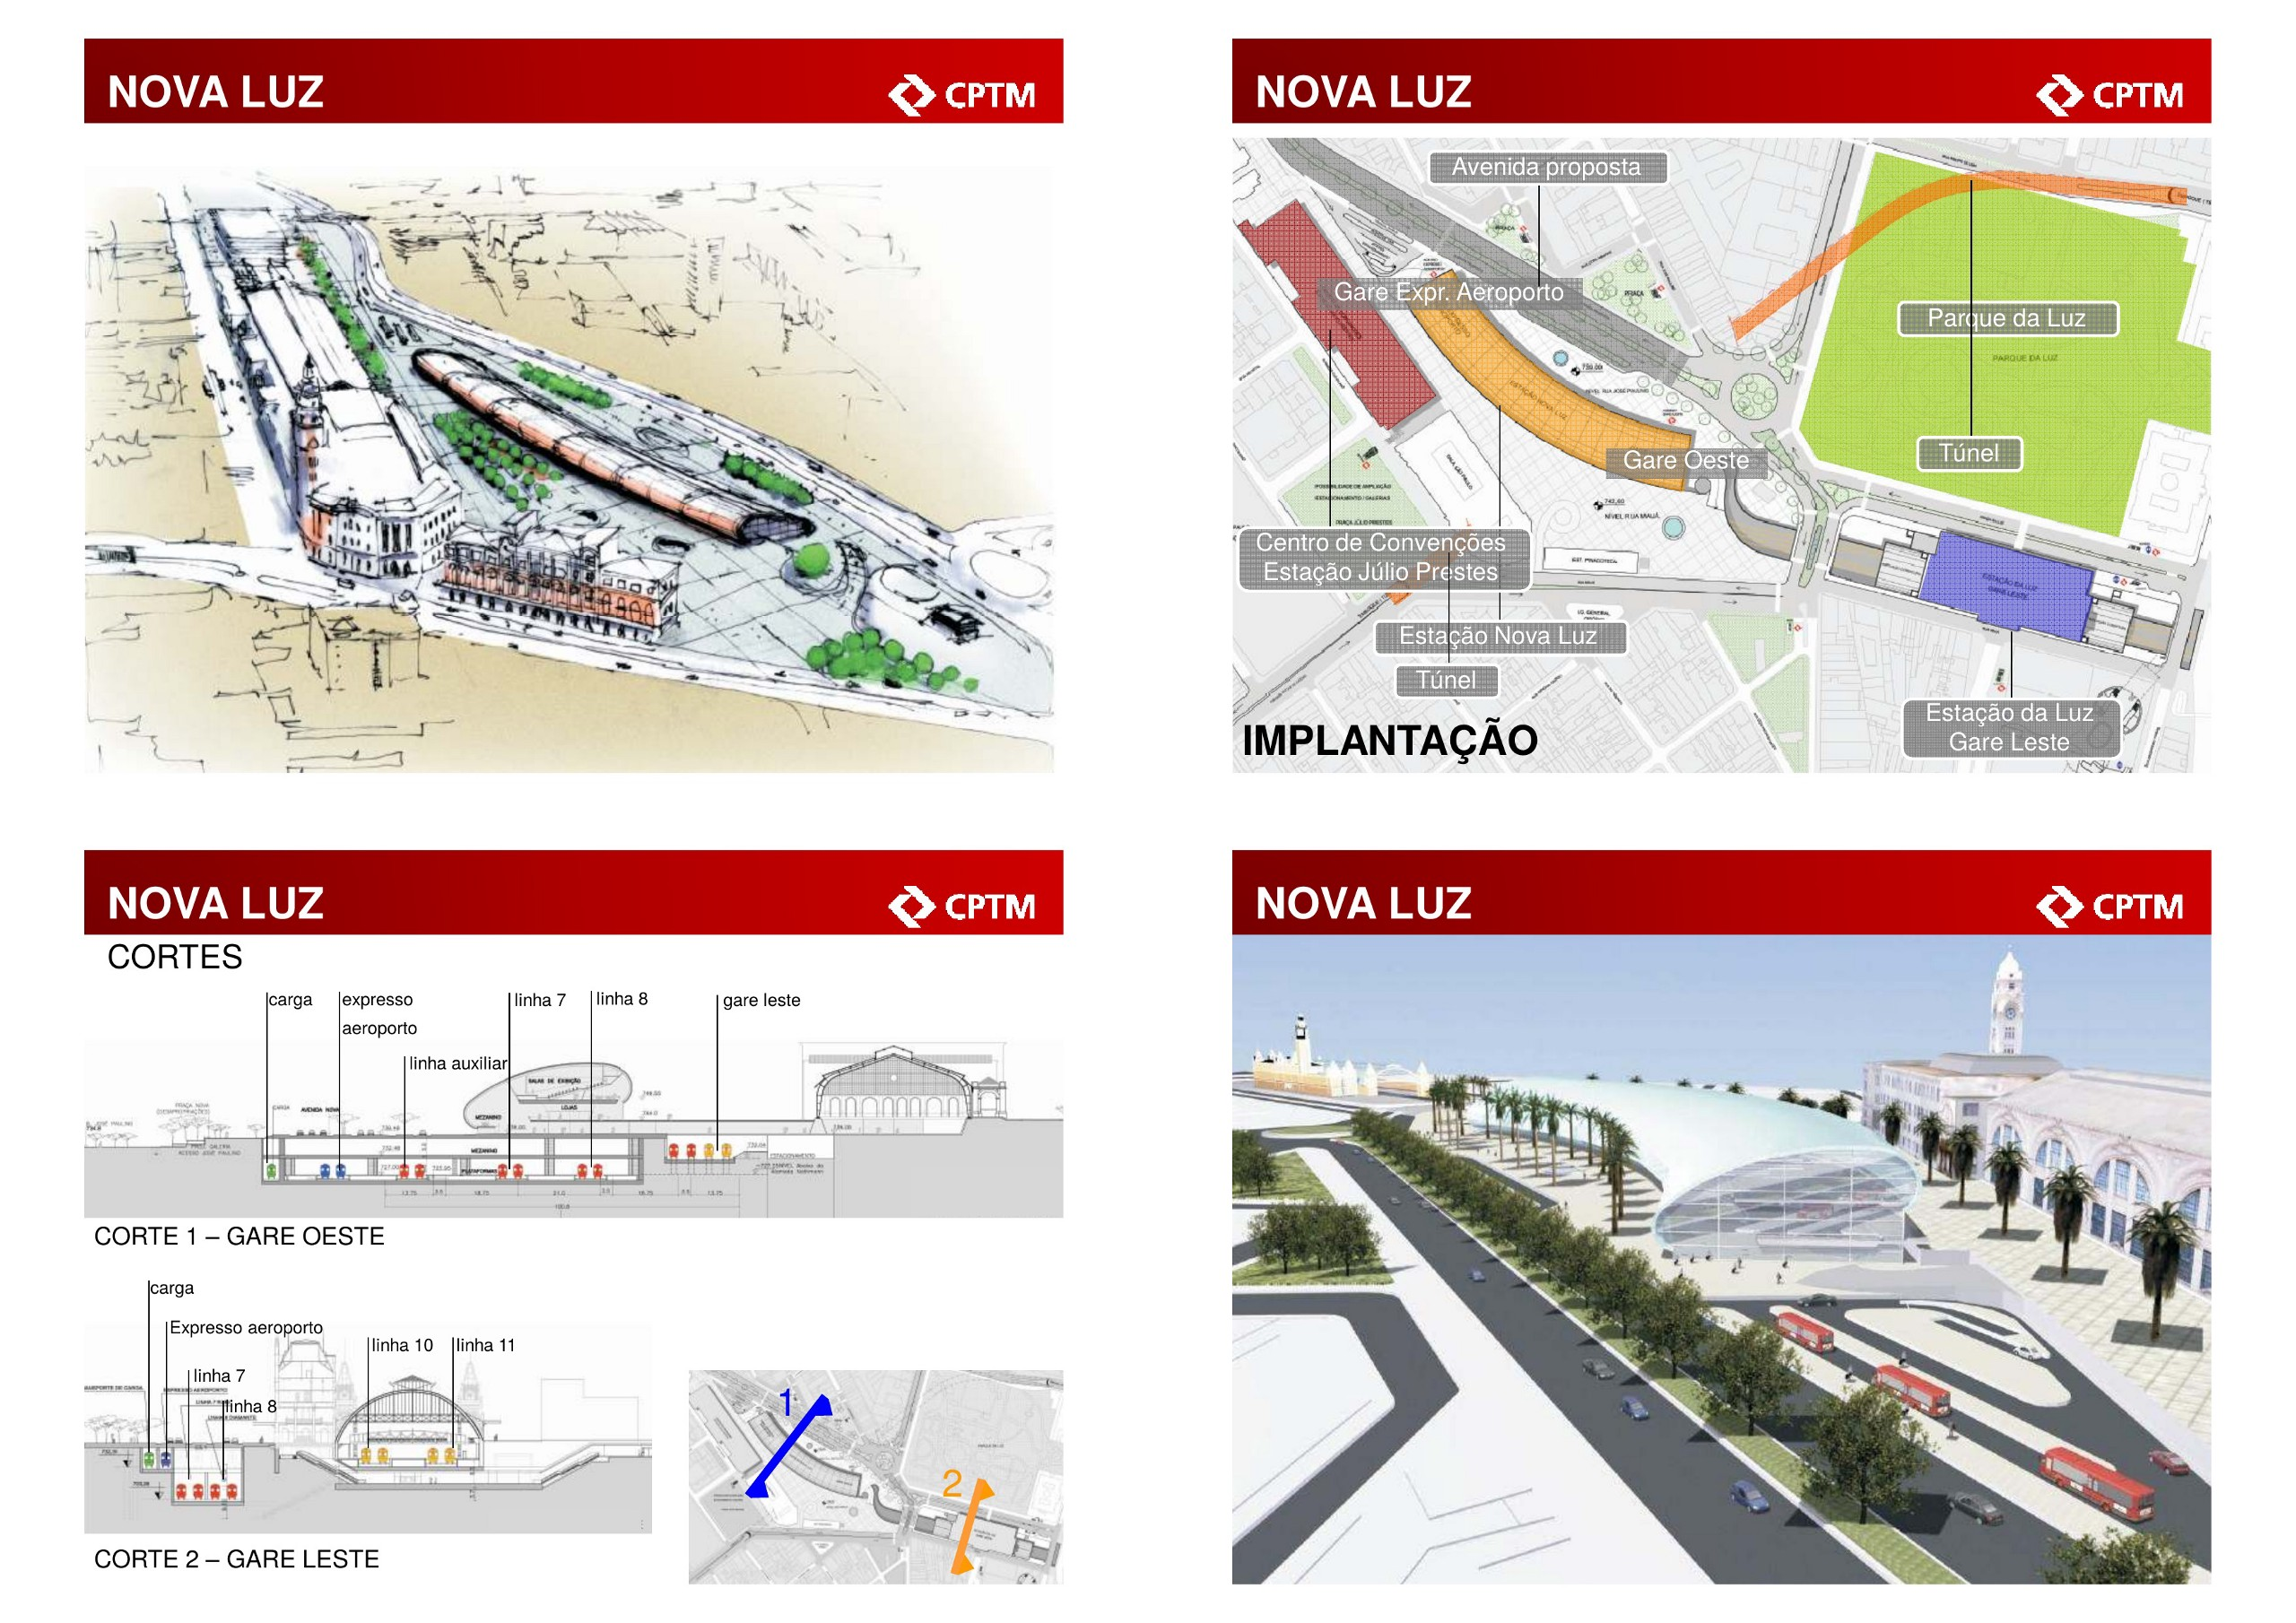
\includegraphics[width=20cm]{slides_nova_luz}
	\label{fig:slides_nova_luz}
\end{figure}
\end{landscape}

Pouco transparente, a \gls{cptm} não precisa datas para seus projetos, não publica cronogramas e não conduz pesquisas com usuários, também parece avessa à participação popular.

Comentamos sobre o projeto de enterramento dos trilhos feito pela Fupam em outro texto. Vale a pena conferir o vídeo do projeto, que permite ter uma visão rápida sobre a proposta:

%TODO ver o que fazer com o texto sobre os 130 km dentro da capital

\subsubsection{O pico}

O horário de pico na Estação Luz é ruim, ele se estende por horas, sendo possível evidenciar desconforto mesmo por volta das 19h. É possível afirmar que o pico já está consolidado por volta das 17h.

Podemos resumir os problemas da estação como sendo:

\begin{itemize}
	\item Embarque perigoso, uma vez que as plataformas laterais têm dimensão problemática, limitando a instalação de organizadores de fluxo. Uma situação ideal poderia implicar na instalação de portas de plataforma;
	\item Escadas insuficientes na plataforma central, tornando o desembarque no pico da manhã arriscado, uma vez que a plataforma não esvazia devido ao baixo intervalo praticado hoje (na Linha 11, beira os 4 minutos em média). Usuários não respeitam a faixa amarela e se arriscam a medida que os trens deixam a plataforma;
	\item Corredor de integração com dimensões reduzidas e com organização deficiente na chegada ao saguão da \gls{cptm}, com conflitos entre quem se dirige ao Metrô no contra-fluxo
	\item Nos picos a transferência entre as linhas 7-Rubi e 11-Coral pode ser desafiadora, uma vez que a maioria se dirige às linhas do Metrô;
	\item Buscando otimizar o fluxo do corredor de integração a \gls{cptm} fechou todas as lojas existentes, mas não liberou o espaço, reforçando o fracasso do projeto original
	\item O balcão de informações fica numa área ruim, muito próximo do acesso ao corredor de integração;
	\item A área livre da estação funciona como ponto de prostituição e a \gls{cptm} demonstra conivência, uma vez que não coíbe a prática mesmo em plena luz do dia.
\end{itemize}

No horário de pico filas se formam nas escadas de acesso às plataformas, principalmente na Linha 11. Como explicado, a plataforma tem dimensões limitadas os acessos a ela foram concebidos num cenário de demanda muito diferente do atual. Mesmo com o desligamento das escadas o acúmulo é inevitável.

É evidente que a \gls{cptm} não sabe mais o que fazer. Se ela tentar limitar o fluxo no corredor, ponto crítico, superlota a Estação Luz da Linha 1-Azul do Metrô. É crucial que a empresa pense numa gare adicional ou pelo menos um novo projeto integrador, contemplando a Estação Júlio Prestes. É o preço dos equívocos feitos anteriormente, que só aumenta com a manutenção do cenário.

\subsubsection{Conclusão}

A Estação Luz da \gls{cptm} é belíssima, um marco no Centro de São Paulo, que impressiona não só pela beleza de sua arquitetura centenária, mas também pela versatilidade proporcionada pelas conexões ali existentes. O problema é que o projeto que levou à sua restauração e modernização foi feito de maneira tacanha.

O plano diretor de inserção urbana da rede da \gls{cptm}, feito pela Fupam, bem como o projeto de enterramento, aparentemente foram demonstrações de que a estatal estava entrando nos trilhos, até que algo aconteceu e ela descarrilou. Kassab enfrentou dificuldades com o Nova Luz (nada surpreendentes pela forma como conduziu o processo), mas as dificuldades com o Nova Luz não poderiam, devido à questão dos CEPACs (certificados de potencial adicional de construção, que permitiram ao município angariar fundos para colocar no projeto de enterramento), motivar o engavetamento da parte que cabia à \gls{cptm}. É utópico, na conjuntura atual, esperar que a capital custeie fortemente o enterramento de uma infraestrutura que não pertence a ela, principalmente quando houve, para variar, passividade do Governo do Estado, que esperou cerca de 10 anos para pensar em algo, se mostrando incapaz de levar a empreitada adiante.

A superlotação e os gargalos na Estação da Luz \textemdash\ e também no eixo Brás-Lapa \textemdash\ só têm se agravado com a postura do governo estadual e da Secretaria dos Transportes Metropolitanos.

\begin{info}
	\infocaio{01/03/2015}{https://goo.gl/r9Xeok}
\end{info}

\section{Estação Ipiranga}\label{s:ipg}

%TODO inserir fotografias

O verão praticamente já começou e as chuvas características também. Infelizmente a Estação Ipiranga, com sua estrutura de quase 60 anos, não é uma das mais confortáveis para ser acessada quando está chovendo.

As plataformas não são totalmente cobertas e poças de água se formam com grande facilidade. Para quem não usa algum tipo de bota, é preciso ter cuidado para não molhar os pés, para não falar do risco de acidentes por escorregamento.

Outro problema da estação é que o principal acesso, voltado a uma praça que se encontra favelizada e fica a poucos minutos a pé do Mooca Plaza Shopping e do Sonda, na Av. Capitão Pacheco e Chaves, entre os bairros da Mooca e da Vila Prudente, tem sérios problemas de drenagem.

Em 13/12/2018, foi possível registrar como se encontrava a passagem de nível que precisa ser obrigatoriamente atravessada para seguir pelo corredor que dá acesso à estação.

Em estações mais modernas da \gls{cptm}, provavelmente o mezanino e o conjunto de passarelas evitaria o contato com a passagem de nível e o pátio de caminhões de carga, porém, por se tratar de uma estação da EFSJ, que foi construída quando ainda existiam trens de longo percurso e quando o serviço suburbano ainda não estava em processo de conversão para um serviço de metrô, a mentalidade era outra, até porque, a estação ficava no meio de um complexo industrial ligado à presença de nomes como a Ford, que fabricava por ali modelos como o Landau. Não existiu preocupação em dotar a estação de melhor acessibilidade e de uma infraestrutura mais confortável para o público operário que dela se utilizava na época.

A situação da Estação Ipiranga é reflexo do impasse relacionado ao Expresso ABC, que nunca saiu do papel (a predileção por fazê-lo por meio de uma PPP parece ter só contribuído para o impasse). Problemas similares podem ser observados em outras estações na mesma época, como Mooca, São Caetano, Utinga, Prefeito Saladino e Santo André.

\begin{figure}[htb]
	\caption[Valor corrigido do Expresso ABC]{Implantação do Expresso ABC poderia custar mais de 1 bilhão atualmente corrigindo pelo IPC-A. Fonte: Calculadora do cidadão do Banco Central do Brasil}
	\centering
	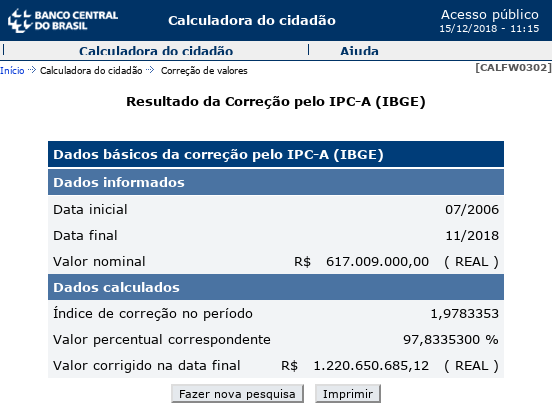
\includegraphics[width=10cm]{calc_bcb_eabc}
	\label{fig:calc_bcb_eabc}
\end{figure}

% fonte da calculadora: https://www3.bcb.gov.br/CALCIDADAO/publico/exibirFormCorrecaoValores.do?method=exibirFormCorrecaoValores&aba=1

A implantação do Expresso ABC está longe de ser trivial: em notícia oficial de 7 de julho de 2006, o custo de implantação do era de R\$ 617,9 milhões (ou R\$ 1.220.650.685,12, corrigindo o valor por meio do IPC-A/IBGE até 7 de novembro de 2018), soma-se ainda o fato de que, para a \gls{cptm} mexer no plano de vias da Linha 10-Turquesa é preciso autorização da União.

Como temos divulgado e opinado desde 2015, o Grande ABC precisa de uma ligação expressa e a faixa de domínio propicia facilidades para a implantação que não são encontradas em outras linhas, ou seja, mesmo custando mais de R\$ 1 bilhão, ainda assim a complexidade é menor do que tentar a empreitada em outras linhas.

Com a predileção privatista do novo governador de São Paulo, João Doria, o momento é de máxima atenção para evitar sucateamento e contratos ruins, pois a chance de todo o sistema ser concedido à iniciativa privada é muito grande e, infelizmente, apelos para isso não são tão difíceis de serem encontrados (vide \autoref{fig:twitter_captura01}).

\begin{wrapfigure}{l}{0.5\textwidth}
	\centering
	\caption[Tuíte pró-privatização da Linha 10]{Usuário acredita que as inundações na Linha 10 serão resolvidas com uma ``privatização''}
	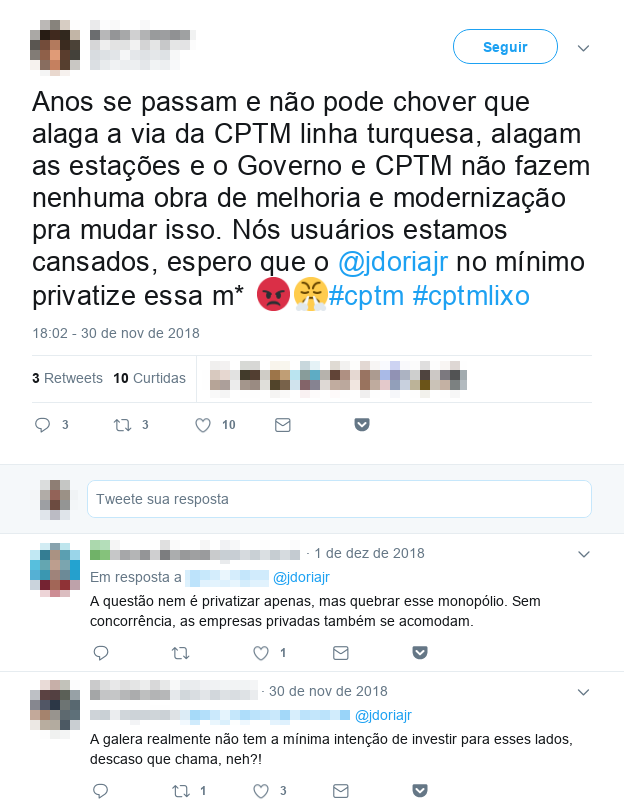
\includegraphics[width=0.9\linewidth]{twitter_captura01}
	\label{fig:twitter_captura01}
\end{wrapfigure}

A Linha 10-Turquesa precisa de investimentos que não serão fáceis de serem conseguidos diante do atual momento vivido pelo país e pelo estado (para consultar séries históricas de execução orçamentária, clique aqui), entretanto, o DCI informou em outubro que “a arrecadação do Estado de São Paulo somou R\$ 111,615 bilhões entre janeiro e agosto deste ano, um aumento real (descontada a inflação) de 2,6\% em relação a igual período do ano passado”. Se uma concessão aparecer no horizonte como algo inevitável, é preciso garantir que o Expresso ABC esteja entre as contrapartidas a serem exigidas da concessionária, bem como a reconstrução das estações depois de Tamanduateí, além da reconstrução das estações Mooca e Ipiranga.

\begin{info}
	\infocaio{16/12/2018}{http://bit.ly/2QUgzQt}\\
	\textbf{Agradecimentos:} Ivo Ramos (indicação da notícia de 2006 sobre o Expresso ABC)
\end{info}

\section{Estação Tamanduateí}

\subsection{Desindustrialização}

A Linha 10 conecta subcentros regionais que atraem grande interesse para viagens, uma vez que concentram empregos e serviços, atraindo não só a população das cidades atendidas, como Mauá, Santo André e São Caetano, mas também da própria capital, São Paulo\cite[pág. 66]{Ferreira}. Como explica \cite[pág. 115]{Stefani}: ``ocorre aqui, uma situação interessante no processo de industrialização paulista. Apesar de ser o sistema rodoviário, instalado no ABC paulista, o responsável pela implantação de diversos setores industriais em São Paulo, como o de mecânica, metalurgia, elétrica e química, tais setores continuam ainda a se instalar no eixo ferroviário e, de certa forma, determinar o crescimento da cidade'', contudo, o mesmo processo não se sustentou em São Paulo, o que se traduz na subutilização do solo urbano ao longo da orla ferroviária após a divisa São Caetano-São Paulo.

\begin{figure}[h]
	\caption{Mapa da rede afixado dentro de um trem da \gls{cmsp}, com parte da Linha 10 visível, de Brás até Utinga (2015)}
	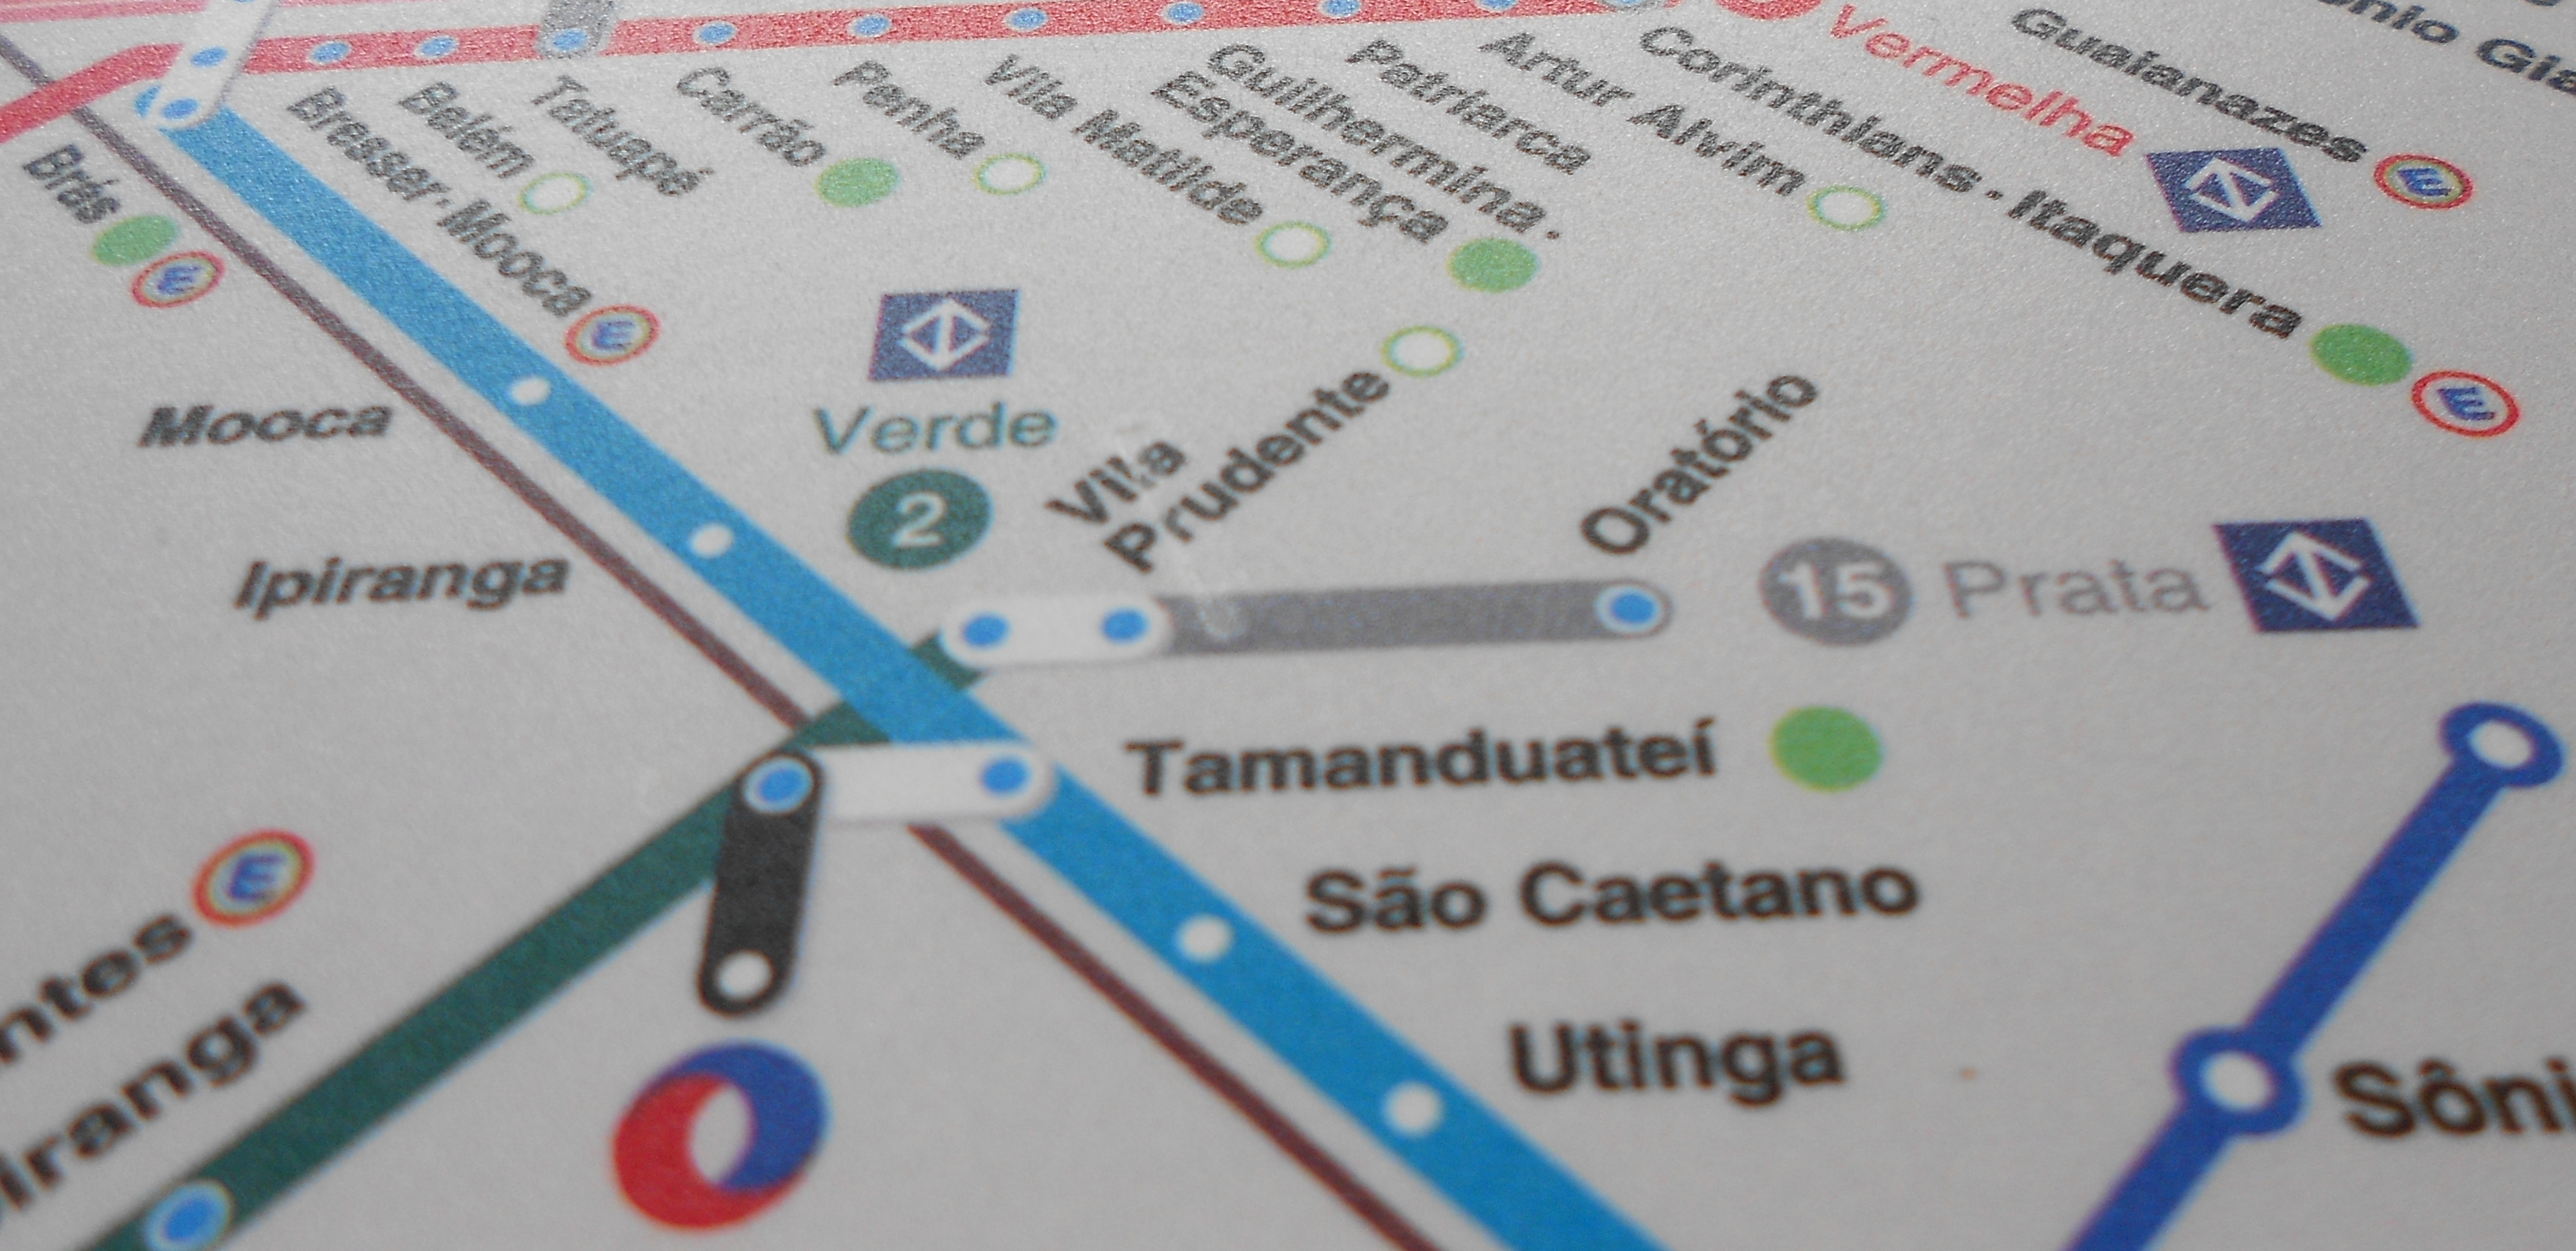
\includegraphics[keepaspectratio,width=\textwidth]{DSCN5732.JPG}
\end{figure}

As metrópoles são o palco em que se dão os movimentos de rearranjo das atividades produtivas deprimidas pela suplantação do fordismo e pela desterritorialização/desindustrialização de corte neoliberal\cite{Acselrad}. A Linha 10 da \gls{cptm} é um espelho do impacto dos movimentos mencionados, sendo visíveis as glebas industriais subutilizadas ao longo das Estações Tamanduateí, Ipiranga e Mooca, estações aqui utilizadas para definição do caso da Linha 10.

\begin{figure}[h]
	\caption{Estação Mooca (2016)}
	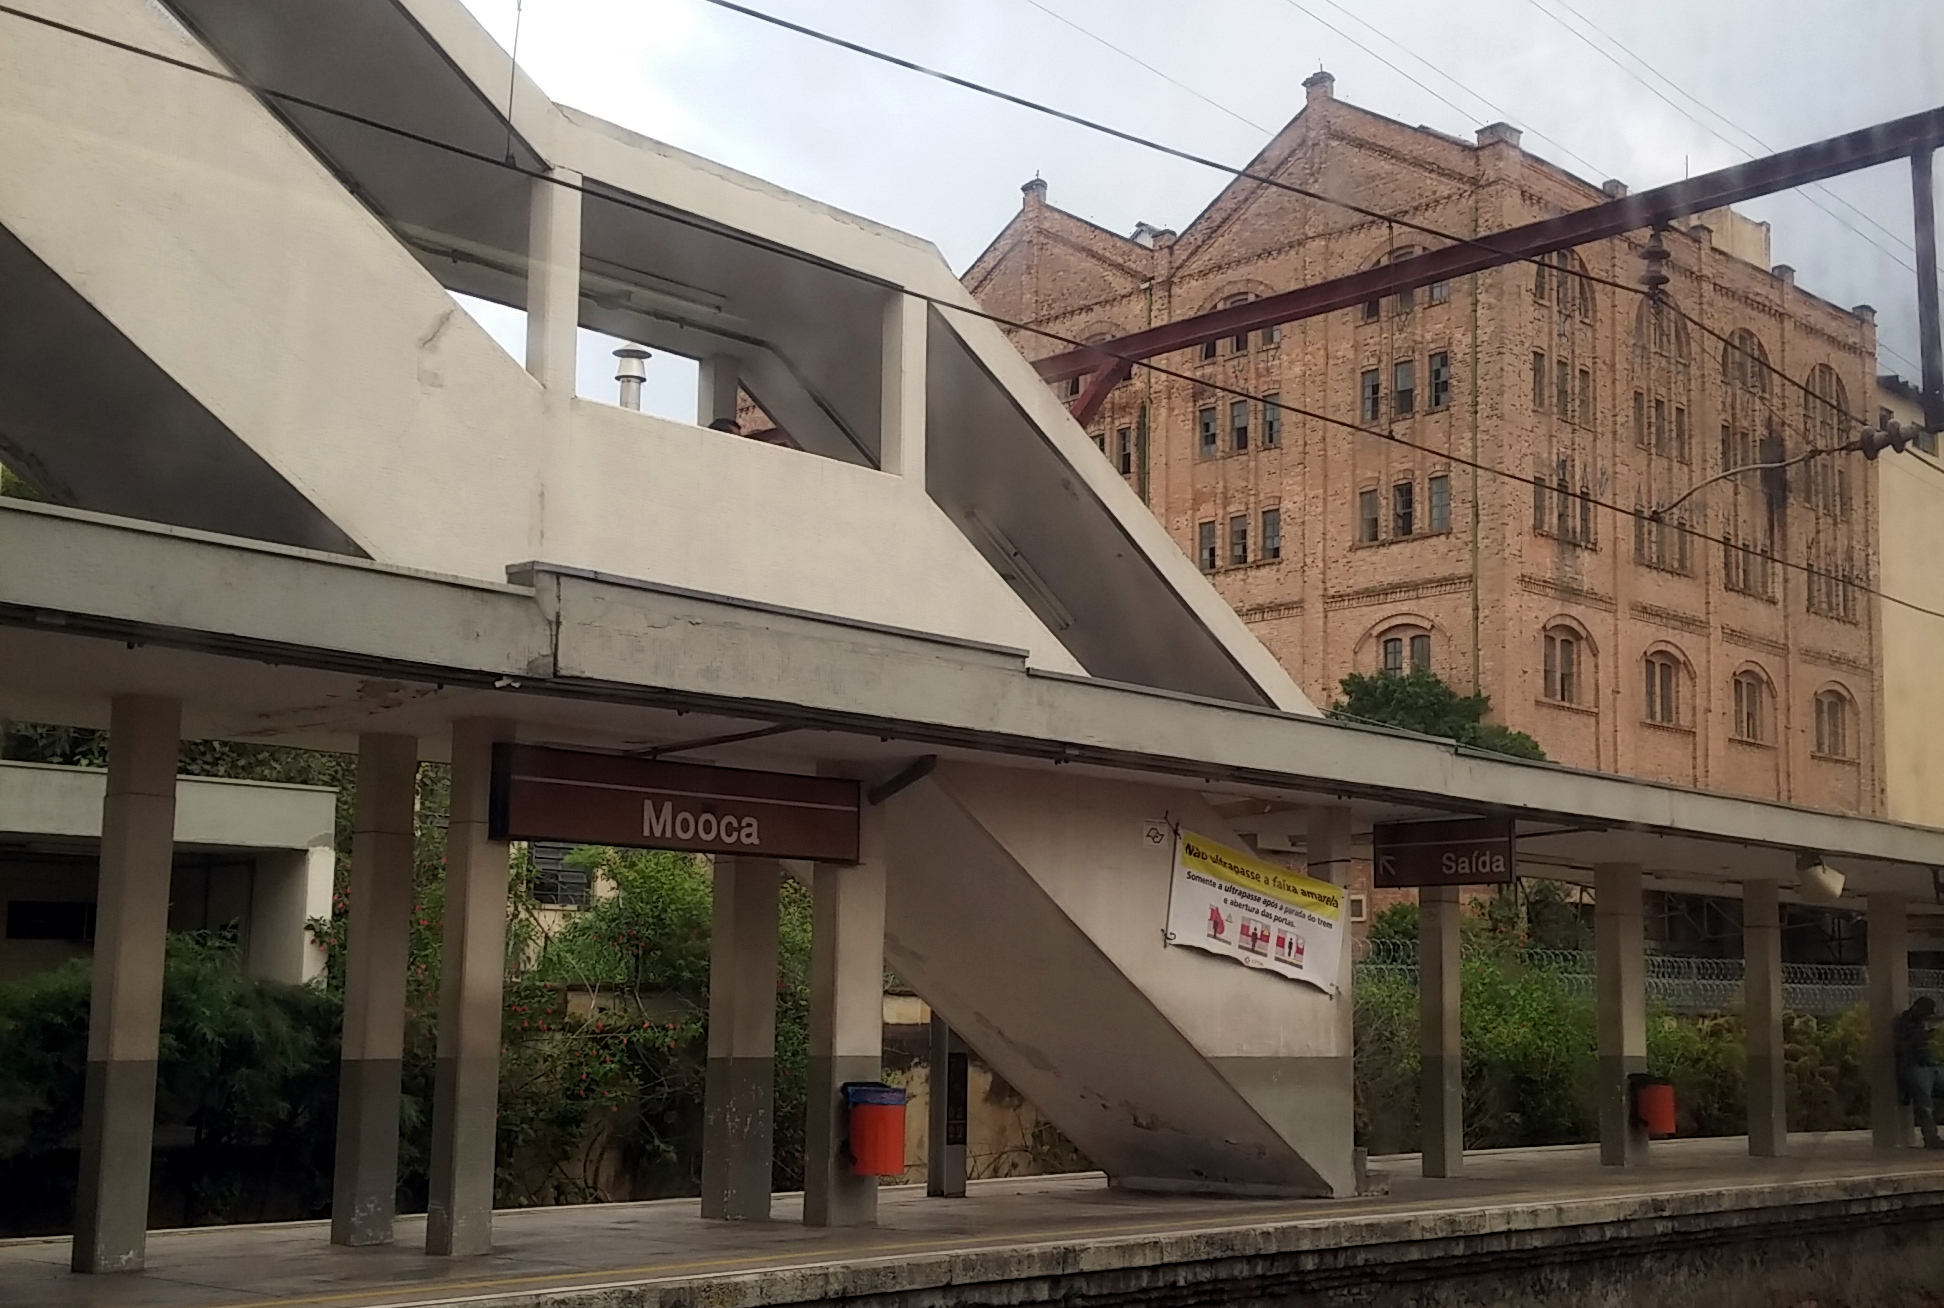
\includegraphics[width = \textwidth]{IMG_20160317_165438b.jpg}
\end{figure}

A visibilidade que menciono no parágrafo anterior é um indicador do descolamento entre uma ferrovia metropolitana com alta capacidade de transporte de passageiros e a orla ferroviária, visto que o acesso às estações acaba sendo prejudicado, bem como seu diálogo com as pessoas, imóveis e equipamentos públicos e privados ao redor. No fragmento abaixo, \cite{Acselrad} fornece uma explanação que ajuda a compreender tal descolamento:

\begin{citacao}
	Em contexto de acumulação flexível, a intensificação e variabilidade temporal do uso de recursos ambientais ameaça a estabilidade do “metabolismo urbano”. Conforme sublinha Veltz, a metrópole acelera a divisão do trabalho e a diversificação contínua dos bens e serviços, constituindo-se em lugar privilegiado do redesenvolvimento de sistemas produtivos doravante ultradecompostos. A economia da velocidade e da incerteza, associada a uma demanda cada vez menos previsível, destrói e recria em permanência o território social. Dadas as altas taxas de juros que tornam o peso fundiário das operações muito elevado, o urbanismo just-in-time de mercado – aquele protagonizado pelas próprias empresas – tende a ser cada vez menos regulamentar e cada vez mais comandado pelas	lógicas do capital imobiliário \cite{Acselrad}. Tudo que diz respeito ao ordenamento espacial regulamentar da cidade, inclusive suas dimensões ecológicas, se esvai em ausência de forças de coordenação, que são eventualmente substituídas pela auto-organização da	“governança corporativa”, da parceria privado-privado, ou seja, em parte crescente, pelos próprios capitais em competição.
	(\cite[pág. 31]{Acselrad})
\end{citacao}

\subsection{Bairros do Tamanduateí}

A região de atendimento da Linha 10 que estou abordando aqui é objeto de uma \gls{ouc} da Prefeitura de São Paulo. A municipalidade tem em andamento a \gls{ouc} Bairros do Tamanduateí. Destaco dois parágrafos da plataforma Gestão Urbana SP que versam sobre a operação:

\begin{citacao}
	A intervenção tem origem nos estudos da Operação Urbana Diagonal Sul, prevista no Plano Diretor Estratégico de 2002, complementados em 2011 por um Consórcio de empresas capitaneadas pelo escritório Vigliecca e Associados, sob contrato da SMDU. Os estudos então desenvolvidos compreenderam o Plano Urbanístico Específico, o Estudo de Capacidade de Suporte da Infraestrutura de Mobilidade, o Estudo de Avaliação Econômica, o Plano de Comunicação, o Estudo de Impacto Ambiental e o respectivo Relatório de Impacto Ambiental.
	
	Confirmada pelo novo Plano Diretor Estratégico, aprovado pela Lei 16.050 de 31 de julho de 2014, a OUC Bairros do Tamanduateí abrange quase a totalidade do Arco Tamanduateí, um dos Setores da Orla Ferroviária e Fluvial da Macroárea de Estruturação Metropolitana.
	(\cite{smdu})
\end{citacao}

Devido ao passado da linha, sua vocação como via de escoamento de carga e de transporte de mão de obra operária continua mostrando sinais que sobrevivem até os dias atuais. Na capital, as glebas industriais há muito perderam força, dando início a discussões sobre o que fazer em bairros como a Vila Carioca (distrito da Moóca), as quais continuam reacendendo a questão da \gls{cptm}, que inclusive chegou a contratar um estudo junto ao UNA Arquitetos para o eixo Moóca-Ipiranga, para o qual:

\begin{citacao}
	Diante da nova inscrição territorial e mudança qualitativa da indústria em São Paulo, o destino de algumas áreas centrais na cidade se tornou objeto urgente de estudo por parte do poder público. A questão é comum à extensão das linhas férreas e coincide com o seu processo de modernização.
	
	O setor Mooca e Ipiranga, cortado pela Avenida do Estado, poderá ser reestruturado a partir desses enormes terrenos vagos. Esses vazios permitem uma nova ocupação que aproxima a população de redes infra-estruturais instaladas. Ao mesmo tempo esses espaços residuais concentram estratos diversos de formação da cidade que merecem ser preservados. O projeto se coloca em sentido de continuidade com os diferentes fluxos da cidade existente, propondo um processo de acumulação de vários tempos em um mesmo espaço. Em contraposição a uma ocupação imobiliária em curso, que segrega e apaga esses vestígios.
	\cite{unaarq}
\end{citacao}

Legalmente, para que a \gls{ouc} fosse possível, o poder público local da capital definiu o Arco Tamanduateí, o qual está incluído na Macroárea de Estruturação Metropolitana. Fora da macroárea não é possível desenvolver uma operação urbana, que no caso do Arco Tamanduateí, é considerado pela \gls{smdu} um dos principais instrumentos de transformação\cite{smdumacro}.

\begin{figure}[h]
	\caption{Estação Tamanduateí (2016)}
	\includegraphics[keepaspectratio,width=\textwidth]{DSCN7465.JPG}
\end{figure}

A Estação Tamanduateí é, até o momento da impressão do livro, a mais moderna de toda a Linha 10-Turquesa, representando avanços drásticos em relação àquelas que estão localizadas no Grande ABC, principalmente. Trata-se de uma estação intermodal, com conexão à Linha 2-Verde do Metrô, além de acesso a ônibus municipais e intermunicipais. Sua construção, no entanto, não representou alterações significativas na região em que se insere, assim, além dos ônibus, sua articulação com o entorno se limita sobretudo ao acesso facilitado a um centro comercial vizinho (Central Plaza Shopping) de uma das faces da estação. Assim como as estações Mooca e Ipiranga, ela está inserida no Arco Tamanduateí e, por conseguinte, na \gls{ouc} Bairros do Tamanduateí.

\begin{center}
	\begin{longtable}{|l|l|p{5.3cm}|p{4.5cm}|}
		\caption{Tabela com as linhas de ônibus na Estação Tamanduateí}\\
		\hline
		\textbf{Linha} & \textbf{Tipo} & \textbf{Viagem de Ida} & \textbf{Viagem de Volta} \\
		\hline
		\endfirsthead
		\multicolumn{4}{c}%
		{\tablename\ \thetable\ -- \textit{Continuado da página anterior}} \\
		\hline
		\textbf{Linha} & \textbf{Tipo} & \textbf{Viagem de Ida} & \textbf{Viagem de Volta} \\
		\hline
		\endhead
		\hline \multicolumn{4}{r}{\textit{Continua na próxima página}} \\
		\endfoot
		\hline
		\endlastfoot
		045 & \gls{emtu} & Santo André (Vila Palmares) & São Paulo (Tamanduateí) \\
		3134-10 & \gls{sptrans} & Shopping Aricanduva & Metrô Tamanduateí \\
		4031-10 & \gls{sptrans} & Pq. Santa Madalena & Metrô Tamanduateí \\
		5110-41 & \gls{sptrans} & São Mateus & Metrô Tamanduateí \\
		%\hline
	\end{longtable}
\end{center}

Segundo informações da plataforma de transparência ``PlanejaSampa'' da Prefeitura de São Paulo, a Meta 123 do Programa de Metas 2013-2016 é a responsável por ``Aprovar a Operação Urbana Bairros do Tamanduateí, a revisão da Operação Urbana Água Branca e iniciar os estudos do projeto Arco Tietê'', tendo sido, conforme dados de 17/12/2015, marcada como concluída, com 100\% dos objetivos atingidos (\cite{smg123}).

Amparando-se no \gls{pl} nº 723/2015, que estabelece ``objetivos, diretrizes, estratégias e mecanismos para a implantação da Operação Urbana Consorciada Bairros do Tamanduateí, define Projeto de Intervenção Urbana para a área da Operação Urbana Consorciada e autoriza a criação da empresa Bairros do Tamanduateí S/A'' (\cite{pl723}), a \gls{smdu} resumidamente determina as seguintes premissas para a \gls{ouc} (\cite{smdu2014}):

\begin{itemize}
	\item Cidade compacta: moradia e emprego próximos;
	\item Áreas verdes acessíveis numa caminhada de 15 minutos;
	\item Uso misto nos imóveis, com fachadas ativas;
	\item Integração tipológica, garantindo convivência entre o tecido atual e novas edificações;
	\item Maior mobilidade e maior qualidade urbana.
\end{itemize}

Concluindo, as intervenções propostas são faseadas e devem se estender por cerca de 50 anos até elevar as unidades residenciais para 83.958 (estoque de 3.964.499 m$^2$), os leitos hospitalares para 1.540 (ante 366), creches/pré-escolas para 101 (ante 34) e as escolas de ensino fundamental e médio para 45 (ante 22), além disso, o plano prevê um aumento de 138\% de áreas verdes (6 novos parques), além de outras ações ligadas ao viário e drenagem (\cite{smdu2014}).

\begin{figure}[h]
	\caption{Cenário temporal 2046: situação final (\cite{smdu2014})}
	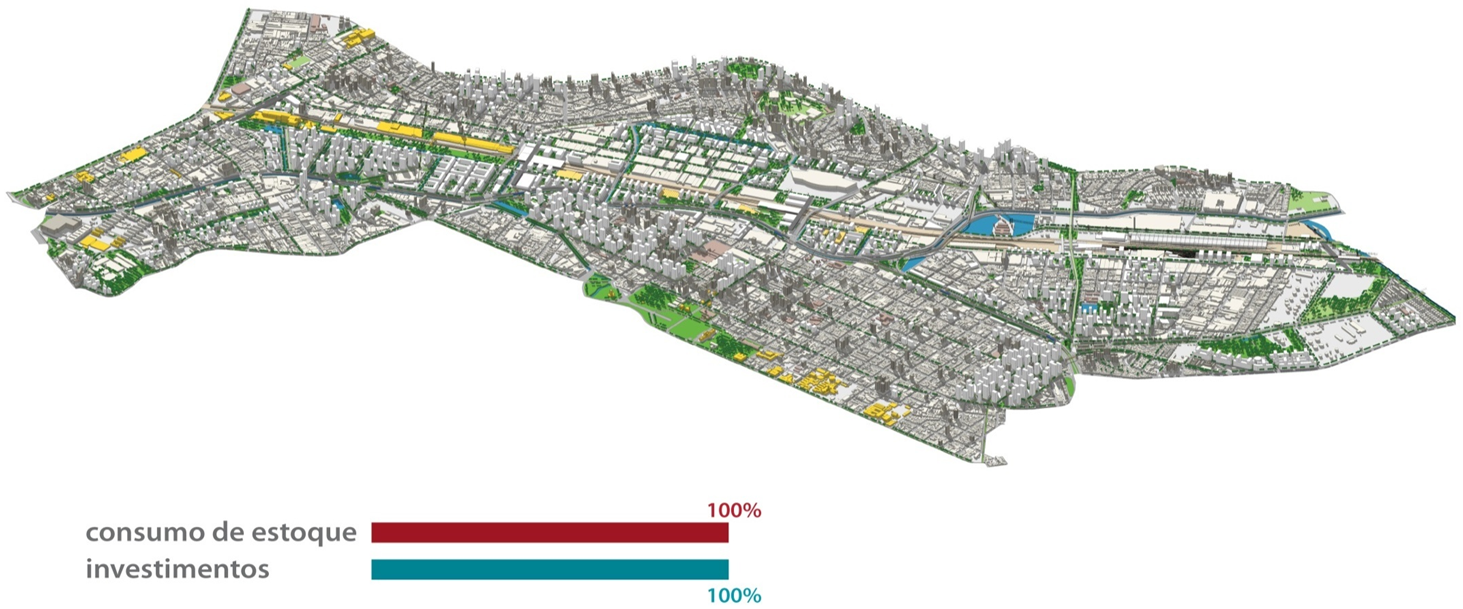
\includegraphics[keepaspectratio,width=\textwidth]{oucbt_consolidado.png}
\end{figure}

\subsection{Alguns dados}

Conforme dados do \cite{ibgeXSP}, São Paulo tem uma população de 11.253.503 habitantes e possui um território com 1.521.110 km$^2$, atendido por 46 estações (\cite{sitecptm1}), das quais 3 foram mencionadas aqui (6,5\% do total de estações da \gls{cptm} no município).

As estações Mooca e Ipiranga possuem um perfil de demanda bastante distinto de Tamanduateí, não sendo nós intermodais, uma vez que não contam com quaisquer facilidades para conexão com ônibus ou, num sentido de maior peso, conexão com outra linha de alta capacidade, como a Linha 2-Verde, acessível por meio da Estação Tamanduateí. A diferença no perfil de demanda exigiu a separação da Estação Tamanduateí no gráfico que veremos a seguir.

\begin{center}
	\begin{longtable}{|p{2cm}|p{3cm}|p{3cm}|p{3cm}|}
		\caption{Demanda do grupo de estações da Linha 10\, baseado em Mídia \gls{cptm}}\\
		\hline
		\textbf{Média} & \textbf{Mooca} & \textbf{Ipiranga} & \textbf{Tamanduateí} \\
		\hline
		\endfirsthead
		\multicolumn{3}{c}%
		{\tablename\ \thetable\ -- \textit{Continuado da página anterior}} \\
		\hline
		\textbf{Média} & \textbf{Mooca} & \textbf{Ipiranga} & \textbf{Tamanduateí} \\
		\hline
		\endhead
		\hline \multicolumn{3}{r}{\textit{Continua na próxima página}} \\
		\endfoot
		\hline
		\endlastfoot
		2011 & 7.689 & 10.900 & 45.971 \\
		2012 & 8.072 & 10.578 & 53.779 \\
		2013 & 7.950 & 10.620 & 58.093 \\
		2014 & 7.664 & 10.558 & 58.112 \\
		2015 & 6.872 & 9.505 & 57.864 \\
	\end{longtable}
\end{center}

\newpage

\begin{center}
	\begin{tikzpicture}
	\begin{axis}[
	title=Evolução da demanda baseado em Mídia \gls{cptm},
	grid=both,
	scaled ticks=false, tick label style={/pgf/number format/fixed},
	x tick label style={/pgf/number format/1000 sep=},
	y tick label style={/pgf/number format/.cd, set thousands separator={.}},
	legend style={at={(0.5,-0.3)},anchor=north,legend columns=-1},
	ylabel=Passageiros (MDU em milhares),
	xlabel=Ano,
	]
	\addplot coordinates
	{(2011,7689
		) (2012,8072) (2013,7950) (2014,7664) (2015,6872)};
	\addlegendentry{Mooca}
	
	\addplot coordinates
	{(2011,10900) (2012,10578) (2013,10620) (2014,10558) (2015,9505)};
	\addlegendentry{Ipiranga}
	
	\end{axis}
	\end{tikzpicture}
\end{center}

A demanda da Estação Tamanduateí, já em 2011, superava 40 mil passageiros em \gls{mdu}, número que é superior ao de todas as estações abordadas neste trabalho.

\begin{center}
	\begin{tikzpicture}
	\begin{axis}[
	title=Evolução da demanda baseado em Mídia \gls{cptm},
	grid=both,
	ymax=60000,
	x tick label style={/pgf/number format/1000 sep=},
	y tick label style={/pgf/number format/.cd, set thousands separator={.}},
	legend style={at={(0.5,-0.3)},anchor=north,legend columns=-1},
	scaled ticks=false, tick label style={/pgf/number format/fixed},
	ylabel=Passageiros (MDU em milhares),
	xlabel=Ano,
	]
	\addplot coordinates
	{(2011,45971) (2012,53779) (2013,58093) (2014,58112) (2015,57864)};
	\addlegendentry{Tamanduateí}
	
	\end{axis}
	\end{tikzpicture}
\end{center}

\begin{obs}
	Seção fortemente baseada em um trabalho de graduação de uma disciplina da Universidade Federal do ABC.
\end{obs}

\begin{info}
	\infocaio{25/04/2016}{https://github.com/caiocco/ufabc-BH0301}
\end{info}

\section{Estação Aeroporto\textperiodcentered Guarulhos}\label{s:agu}\index{Estação Aeroporto\textperiodcentered Guarulhos}

\subsection{Introdução}

A Linha 13-Jade (Eng. Goulart-Aeroporto) da Companhia Paulista de Trens Metropolitanos (\gls{cptm}) foi aberta ao público pela primeira vez no último sábado, 31, desde então, já ouvimos de tudo um pouco: “não chega no aeroporto”, “não serve para quem usa bagagens”, “não atende a cidade de Guarulhos”, “liga nada ao lugar nenhum” etc.

Até que a expansão da Linha 2-Verde (atualmente Vila Madalena-Vila Prudente) alcance a cidade de Guarulhos, a Linha 13 será a única conexão sobre trilhos entre a capital e a segunda cidade mais populosa da Grande São Paulo. Trata-se, porém, de uma ligação que já nasce com evidentes limitações: a nova linha se conectará com o aeroporto justamente no terminal menos utilizado: o Terminal 4, escolha esta que reflete uma decisão do próprio aeroporto, como veremos a seguir; para piorar a situação, não existe um horizonte de curto prazo para expansão da linha, que ficará confinada por alguns anos na Estação Engenheiro Goulart da \gls{cptm}.

\subsection{Prazos e promessas do poder público}

A ordem de serviço para as obras civis da foi assinada em 2013 com a promessa de conclusão para 2015, postergada depois para 2016, porém as obras realmente só progrediram ao ponto de ser possível a entrega da linha em operação assistida (e limitada, com um único trem operando) no primeiro quadrimestre de 2018. Parte dos recursos vieram da Agência Francesa de Desenvolvimento.

Expresso Aeroporto. É importante apontar que o governo estadual vinha prometendo uma ligação para o aeroporto internacional desde 2002, no entanto, aquele projeto envolvia uma PPP por exigência dos bancos de fomento e a iniciativa privada sempre exibiu desinteresse (veja aqui, aqui e aqui), situação esta que ficou reforçada quando o pouco participativo projeto Nova Luz se mostrou inviável, juridicamente e financeiramente, visto que estava prevista uma estação para uma linha para o aeroporto, que, lembremos também, desde o princípio tinha a proposta de ser um serviço executivo e mais caro. O Expresso Aeroporto, definitivamente morto e enterrado, era conhecido como sendo a Linha 14-Ônix – atualmente o número e pedra preciosa se encontram atribuídos à ligação Guarulhos-ABC que está sendo projetada pela \gls{cptm}.

A confusão entre a Linha 13-Jade e a antiga Linha 14–Ônix ou Expresso Aeroporto, parece ter levado o governador Geraldo Alckmin a falar em mentira quando questionado pela Folha de S.Paulo. O que poderíamos dizer é: a grosso modo, senhor governador, não parece totalmente correto falar em mentira, afinal, a promessa de conexão entre a capital e o aeroporto tem mais de 10 anos. O que não parece ter ficado claro, inclusive para a imprensa, é a distinção entre os tipos de serviço ao longo dos anos, fruto, como apontamos, da predileção por uma iniciativa privada que sempre se mostrou desinteressada. O G1, por exemplo, fala em 14 anos de atraso, sem distinções.

Conforme reportagem do Estadão intitulada “Trem para aeroporto de Cumbica começa a ser construído”, temos a confirmação da assinatura do contrato para as obras civis para atual Linha 13-Jade, que ocorreu quando o governo “jogou a toalha” de vez, sepultando a Linha 14-Ônix:

\begin{citacao}
	Em evento na Estação Palmeiras-Barra Funda, na zona oeste, o governador Geraldo Alckmin (PSDB) assinou a ordem de serviços para que a construção comece. Ele prometeu a entrega da linha, com quase 12 km de comprimento e três estações, para 2015.
	
	No fim do ano passado, o tucano havia afirmado que as obras começariam em março deste ano e que durariam 18 meses, até por volta de setembro de 2014.
\end{citacao}

\subsection{A iniciativa privada também sabe prometer (e não cumprir)}

A mesma reportagem do Estadão explica os motivos da localização da estação do aeroporto, um dos pontos que tem gerado questionamentos nas redes sociais e até mesmo dentro do campo progressista, por pessoas ligadas ao campo da mobilidade de uma forma ou de outra:

\begin{citacao}
	A Estação Aeroporto Internacional de Guarulhos ficará suspensa sobre o canteiro da Rodovia Hélio Smidt e será conectada ao aeroporto por meio do terminal 4, o “puxadinho”, o menos movimentado dos três já abertos. Esse terminal é fisicamente desconectado de todos os demais. Para sanar o problema, a concessionária de Cumbica, a GRU Airport, prometeu construir um “people mover” para transportar gratuitamente os passageiros entre os terminais. Ainda não se sabe se será um monotrilho ou um veículo leve sobre trilhos (VLT).
	
	Fernandes disse que a escolha desse local \textemdash\ e não as imediações dos terminais 1 e 2 ou do futuro terminal 3, que será o maior \textemdash\ se deve ao fato de que a GRU Airport tem intenção de construir ali um shopping center, com fast food e serviços. “Ali na frente do terminal 4, nós vamos fazer uma asa de acesso direto para Guarulhos. Então, a população, através da estação, vai ter acesso ao aeroporto, para fazer uso de cinemas, shopping.”
\end{citacao}

Para piorar, segundo o blog Metrô \gls{cptm}, a concessionária estimava, no final de 2016, 18 meses para entregar um sistema de people mover do aeroporto, conectado à \gls{cptm}, o que não passou de uma promessa, feita por uma concessionária que já demonstrou dificuldades para pagamento da outorga exigida pelo poder concedente:

\begin{citacao}
	Na época, o presidente da concessionária, Antônio Miguel Marques, fez pouco caso da chegada da Linha 13 às proximidades do aeroporto. “Quando a Linha for entregue um dia antes inauguramos o people mover”, registraram alguns jornais. Agora, mesmo com todo atraso da linha da \gls{cptm}, o ‘trenzinho’ da GRU Airport não passa apenas de uma ideia. Segundo reportagem do jornal Folha de São Paulo, a concessionária estima entregar a ligação férrea entre a estação da Linha 13 e os terminais 2 e 3 apenas 18 meses após a abertura do ramal.
\end{citacao}

A GRU Airport demonstra que reavaliou o nível do atendimento que forneceria, como podemos ler em reportagem recente na Folha de S.Paulo, publicada em 31/03/2018:

\begin{citacao}
	O plano era usar um monotrilho, a exemplo de outros grandes aeroportos, mas segundo avaliação da GRU Airport, a demanda de passageiros será suficientemente atendida com o sistema rodoviário \textemdash\ agora consolidado.
\end{citacao}

A reportagem ainda salienta que a concessionária mais uma vez se esquivou de prestar esclarecimentos sobre o shopping que prometeu construir:

\begin{citacao}
	A GRU Airport foi questionada pela Folha, mas não respondeu sobre a previsão de inauguração do shopping, previsto para o terminal 3.
\end{citacao}

Apesar da concessionária garantir que os ônibus seriam suficientes, o COMMU identificou que os veículos circulavam lotados, além disso, o Diário do Transporte também criticou a falta de organização da concessionária. Confira nosso vídeo registrando um pouco da operação dos ônibus (\autoref{qr:video_aeroporto}).

Para registros fotográficos dos ônibus superlotados logo no primeiro dia de operação assistida,confira o tuíte enviado pela Rádio Trânsito e reproduzido na \autoref{fig:twitter_captura02}.

\begin{figure}[htb]
	\caption[Ônibus lotados do aeroporto internacional]{Ônibus do aeroporto lotam no primeiro dia de operação da Linha 13-Jade da \gls{cptm}}
	\centering
	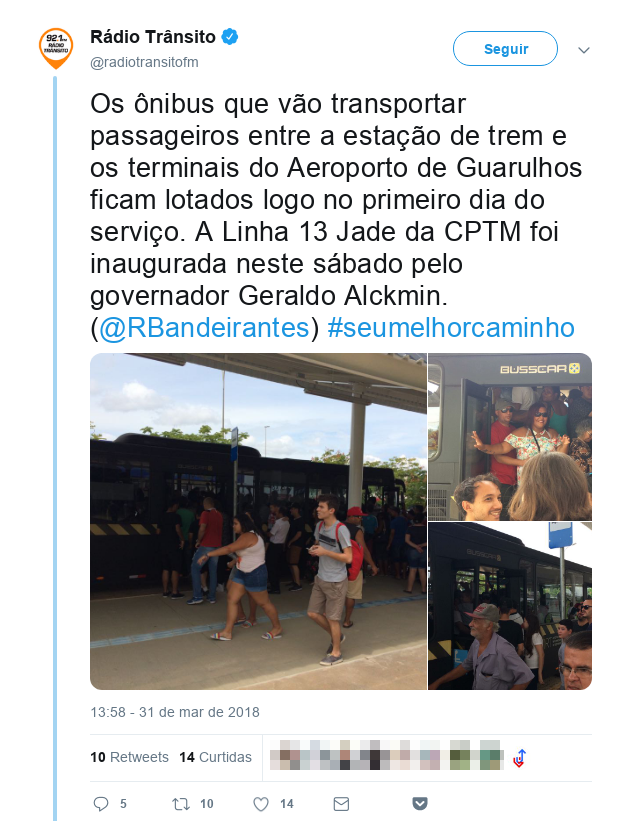
\includegraphics[width=10cm]{twitter_captura02}
	\label{fig:twitter_captura02}
\end{figure}

\subsection{Ligando nada a lugar nenhum}

Afirmar que a Linha 13-Jade liga nada a lugar nenhum é um bocado desrespeitoso com a periferia de São Paulo e também com a periferia de Guarulhos. Veja a seguir algumas considerações estação por estação:

\begin{itemize}
	\item Engenheiro Goulart: nesta estação é possível se transferir para a Linha 12-Safira (Brás-Calmon Viana) e também desfrutar do Parque Ecológico do Tietê;
	\item Guarulhos-CECAP: nesta estação é possível acessar a rodoviária do município de Guarulhos e também parte dos conjuntos habitacionais projetados por Vilanova Artigas, portanto, é uma estação que pode modificar sensivelmente a vida de quem mora naqueles edifícios;
	\item Aeroporto-Guarulhos: além do acesso aos ônibus do aeroporto, cujo tempo de trajeto varia bastante (o acesso ao Terminal 1, que concentra voos domésticos de baixo custo, por exemplo, leva aproximadamente 2 minutos, segundo a concessionária, por outro lado a concessionária diz que chegar no Terminal 3 exige mais de 10 minutos), há também um terminal de ônibus que concentra linhas municipais e intermunicipais, atendendo uma parcela ainda maior da população periférica de Guarulhos.
\end{itemize}

É importante tomarmos cuidado com o significado da expressão em questão para não tratar a periferia como nada. É paradoxal querer chegar num aeroporto que está localizado na periferia ao mesmo tempo que se tenta evitar contato com a infraestrutura que atende aquela mesma região periférica. Simplesmente não dá.

\begin{wrapfigure}{l}{0.5\textwidth}
	\centering
	\caption[QR Code para vídeo dos ônibus do aeroporto internacional em 31/03/2018]{QR Code para vídeo gravado em 31/03/2018, cerca de uma hora antes do término da operação assistida da Linha 13-Jade}
	\qrcode[version=1,height=4cm]{https://www.youtube.com/watch?v=M8haRiSqlGI}
	\label{qr:video_aeroporto}
\end{wrapfigure} 

Também é curioso como o famigerado discurso da “periferia primeiro”, recorrente em discussões sobre as carências na infraestrutura de transporte de massa, mostrou mais uma vez como se esgota rapidamente. Acompanhe o raciocínio: se a periferia tem deslocamentos pendulares e não existem políticas públicas para aumento do dinamismo e redução da pendularidade no horizonte de algumas décadas, implantar linhas que atendem sobretudo a periferia resulta em chacota, com pessoas repetindo o famoso bordão “liga nada a lugar nenhum” \textemdash\ expressão que chegou a ser colocada até numa reportagem da edição brasileira do periódico espanhol El País \textemdash, que até a chegada da Linha 4-Amarela também amaldiçoou a Linha 5–Lilás (então Capão Redondo-Largo Treze), colocando a Linha 9-Esmeralda, bem como as centralidades e pontos de interesse por ela atendidos, num verdadeiro limbo. Pior ainda: não raramente quem vive na periferia adere ao discurso, passando a se marginalizar e marginalizar seu local de residência, ainda que talvez não tenha consciência.

\subsection{Críticas vagas envolvendo a Linha 12-Safira}\index{Linha 12-Safira}

Ainda dentro do tema de como as regiões atendidas pela Linha 13 estão sendo enxergadas, identificamos que blogs manifestaram insatisfação com o nível de serviço da Linha 12-Safira. Foi o caso do Metrô \gls{cptm}, que opinou da seguinte maneira (grifo nosso):

\begin{citacao}
	Na verdade, sua ligação ao restante da rede metroferroviária feita pela Linha 12-Safira é que tira parte da atratividade em usá-la. Exceto pelos trens que seguirão para Brás e também para Luz (com tarifa de R\$ 8 anunciada hoje), os demais pararão na distante estação Engenheiro Goulart onde seguirão viagem pela Linha 12, \textbf{uma das mais precárias da \gls{cptm}}.
\end{citacao}

Entretanto, o autor, Ricardo Meier, em nenhum momento descreve ou fornece referências para enriquecer os pontos que coloca. Por exemplo, ao afirmar que a Linha 12-Safira é precária, não fica claro o que ele pretende insinuar.

Seria a infraestrutura das estações? Exceto pelas estações de Itaquaquecetuba, todas as outras são novas (inauguradas pelo menos na segunda metade dos anos 2000) ou suficientemente atuais, como é o caso da Estação Tatuapé, de 1981.

Seria o intervalo? Durante a permanência do COMMU nas estações Engenheiro Goulart e Tatuapé, não foram observados intervalos insatisfatórios: a linha aparentava estar operando dentro da média de um trem a cada 8 minutos, justamente a esperada para um sábado sem obras, no período das 4h às 19h. A tabela completa com os intervalos da Linha 12-Safira pode ser consultada aqui.

%TODO reproduzir tabela de intervalos aqui

Parece um exercício de crítica genérica pela crítica genérica: a repetição de um estigma ou uma crítica muito generalista, o que no final das contas acaba contribuindo para marginalizar a \gls{cptm}, seus passageiros e as regiões atendidas.

\subsection{Planos para expansão}

Ao confinar a Linha 13-Jade na Estação Engenheiro Goulart, sua atratividade segue drasticamente reduzida. Exceto pelo Parque Ecológico do Tietê, cujo acesso finalmente foi facilitado com a nova estação, não existe nenhum outro atrativo. A estação está localizada numa área periférica da Zona Leste e os subcentros regionais mais próximos são Tatuapé (no sentido centro) e São Miguel Paulista (no sentido bairro), sendo que o acesso a eles, bem como a qualquer outra estação da rede de trilhos, exigirá que o passageiro utilize a Linha 12-Safira (Brás-Calmon Viana), que por sua vez, termina nas proximidades do Largo da Concórdia, não chegando nem mesmo no Centro Velho.

Elenco os seguintes problemas imediatos:

\begin{itemize}
	\item Infraestrutura hoteleira deficiente, pois o Tatuapé permanece incipiente como centralidade de negócios (o hotel mais próximo da estação homônima não ficou pronto ainda e o segundo mais próximo não tem acesso cômodo);
	\item Saturação elevada de todo o tronco ferroviário pesado da Zona Leste devido à pendularidade (muito lotado no sentido centro pela manhã, muito lotado no sentido bairro pela tarde);
	\item Falta de confiabilidade e previsibilidade nos acessos rodoviários existentes para a parcela que precisa utilizar vias como a Marginal Tietê, uma vez que a última obra realizada nela não considerou qualquer meio coletivo de transporte, sobre trilhos e/ou sobre pneus;
	\item Falta de operações especiais na Linha 12-Safira, o que significa que os trens superlotam em estações ainda mais periféricas e o embarque em estações como USP Leste e Engenheiro Goulart já é difícil hoje.
\end{itemize}

Planos para expansão da Linha 13-Jade já existem, mas os ânimos devem ser contidos até 2016, pelo menos. Num olhar otimista, poderemos ver algum progresso em relação ao tema por volta de 2020. Em setembro de 2013 o Governo do Estado anunciava intenções de expandir o atendimento na cidade de Guarulhos, conforme trecho da notícia “Governo diz que Linha 13 da \gls{cptm} irá além do aeroporto de Guarulhos”:

\begin{citacao}
	O projeto do novo trecho está sendo estudado. Ainda não há definição, por exemplo, do número de estações e do traçado. “A extensão é para o futuro. Porque o trem não vai entrar no aeroporto. O trem vai abraçar o aeroporto, ele vai dar a volta por fora em direção à Vila São João”, informou o secretário, que participou nesta manhã de um evento em Guarulhos. “Se a gente fizer essa linha uma concessão ou uma PPP [parceria público-privada], vai estar contida nesta PPP a extensão para a Vila São João”, afirmou.
\end{citacao}

Para se ter uma ideia de quão limitada a linha nascerá, a \gls{cptm} só prevê um incremento considerável na demanda de passageiros no quinto ano de operação, conforme podemos verificar no slide 18 de uma audiência pública, reproduzido na \autoref{fig:slide_inicio_l13}:

\begin{landscape}
\begin{figure}[h]
	\centering
	\caption[Slide de apresentação sobre a Linha 13-Jade]{Slide 18 de uma apresentação assinada pelo engenheiro Luiz Alfredo Amorim Jr., usada numa audiência pública sobre a Linha 13}
	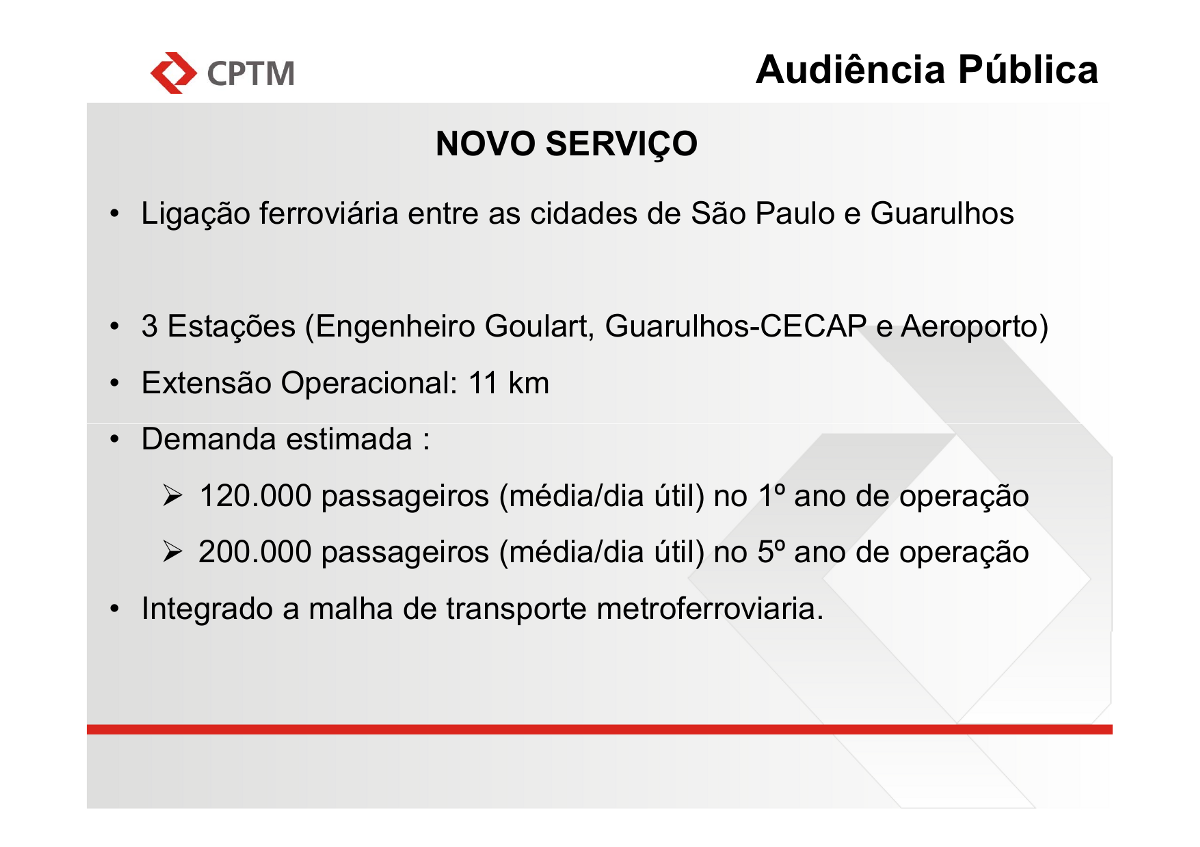
\includegraphics[width=20cm]{slide_inicio_l13}
	\label{fig:slide_inicio_l13}
\end{figure}
\end{landscape}

% http://www.cptm.sp.gov.br/licitacoes/AudienciaPublica/Arquivos/APRESENTACAO_AUD_PUBL_LINHA%2013%20JADE_VF.pdf

Para a Linha 13-Jade, algum otimismo em relação à expansão pode ser justificado pelo fato de existir espaço na faixa de domínio da Linha 12-Safira, ou seja, a implantação de estações em superfície, como a futura Tiquatira, importante pela conexão também futura com a Linha 2-Verde, não deverá impor grandes desafios à \gls{cptm}.

Em informações obtidas com base na Lei Federal nº 12.527/2011, o investimento total será de R\$ 1,8 bilhão. O intervalo médio inicialmente previsto será de 8 minutos e poderá diminuir para até 3 minutos conforme a evolução da demanda, que está projetada para as estações da seguinte forma:

\begin{itemize}
	\item Aeroporto-Guarulhos: 40 mil passageiros por dia;
	\item Guarulhos-CECAP: 36 mil passageiros por dia;
	\item Engenheiro Goulart: 76 mil passageiros por dia.
\end{itemize}

Com relação à intermodalidade Trem Metropolitano-ônibus em Guarulhos, a \gls{cptm} informou o seguinte:

\begin{citacao}
	A \gls{cptm} trata com a prefeitura local para a questão da integração. Esta só ocorre se houver interesse do município. Os estudos de remanejamentos de linhas municipais, obviamente, é de responsabilidade dos municípios.
\end{citacao}

Até a publicação deste livro não há integração tarifária entre os ônibus municipais guarulhenses e a Linha 13-Jade, exigindo o pagamento de duas tarifas cheias, entretanto, faltando três dias para a operação assistida da Linha 13, foram criadas linhas de ônibus em Guarulhos com foco no atendimento de pacientes, todas atendendo o Terminal Metropolitano Taboão e, portanto, conectadas à Linha 13-Jade. São elas: 356A, 356B, 717A e 717B, conforme informações do Guarulhos Hoje\footnote{\url{https://www.guarulhoshoje.com.br/2018/03/28/prefeitura-cria-quatro-linhas-de-onibus-com-itinerario-exclusivo-para-unidades-de-saude/}}.

\subsection{Conclusão}

%TODO atenção para citação de outro artigo do COMMU

Infelizmente a Linha 13-Jade nasce com sérias limitações, dependendo excessivamente da Linha 12-Safira, o que lhe atribui pouca versatilidade em termos de conexões com a rede de trilhos, além disso, tem horizonte de expansão nebuloso, que se agrava pela também nebulosa conectividade com os terminais 1, 2 e 3 do GRU Airport.

É lamentável que o maior aeroporto brasileiro possua a rodovia como único elo entre ele e a metrópole, mas é ainda mais lamentável que se desenhe uma linha tão tacanha para conectá-lo com a malha metroferroviária. A Linha 13-Jade nasce aquém das necessidades não só da capital paulista, mas também de Guarulhos e de outras cidades da Região Metropolitana de São Paulo.

O Governo do Estado demonstrou, mais uma vez, ser pouco visionário e ter um compromisso questionável com a busca por uma rede de alta e média capacidade de excelência.

Não temos dúvidas de que, para a imensa maioria, o impacto da Linha 13-Jade será muito pequeno, apesar dos quase R\$ 2 bilhões que serão gastos para tirá-la do papel.

Como exposto, trata-se de uma ligação bastante limitada, com previsão de demanda tímida e que precisa ser expandida para fornecer um atendimento mais robusto.

A Linha 13-Jade, por bem ou por mal, não deixa de ser interessante para mostrar \textemdash\ escancarar, cá pra nós \textemdash\ que há um longo caminho a ser percorrido quando vamos discutir sobre transporte público e a metrópole, tanto que, às vésperas de sua entrega, os artigos da Linha 13 apresentaram um aumento expressivo nos acessos no Medium do COMMU, apesar de não estarem sendo divulgados há meses (algo como uns 300 acessos por dia na última semana de março de 2018, considerando o artigo ``Linha 13-Jade: uma ligação para Guarulhos que já nasce limitada'').

\begin{info}
	\infocaio{01/04/2018}{http://bit.ly/linha13capenga}
\end{info}

\begin{obs}
	\textbf{Observação:} parte do artigo ``Linha 13-Jade: uma ligação para Guarulhos que já nasce limitada'' foi mesclado, de maneira a concentrar as informações sobre a Linha 13 num único capítulo e seção. O original pode ser acessado em \url{https://goo.gl/eMG1JQ}
\end{obs}

\section{Estação Lapa}

Mesclar artigos sobre enterramento.

\section{Estação Guaianazes}\index{Estação Guaianazes}\index{Linha 11-Coral}

\subsection{Introdução}

A única ligação expressa da Zona Leste e com quase 16 anos de existência, segue repleta de limitações e descumprindo antigas promessas e anseios. Para se ter uma ideia, a inauguração da Estação Suzano foi adiada pela pelo menos nove vezes\footnote{\url{http://www.portalnews.com.br/_conteudo/2016/01/cidades/22919-estado-atrasa-novamente-entrega-e-seqer-tem-data-para-chefa-do-expresso.html}}, embora o contrato, que deveria durar 15 meses, tenha sido assinado em outubro/2010. Como não cutucar a ferida do Expresso Leste, parte da Linha 11-Coral (Luz-Guaianazes-Estudantes) da Companhia Paulista de Trens Metropolitanos?

O Expresso Leste hoje é um trecho com 24 km na Linha 11, no qual o passageiro desfruta integralmente de trens com ar condicionado, baixos intervalos (nos picos, um trem a cada quatro minutos em média) e estações mais modernas, numa ligação paralela à Linha 3-Vermelha (Barra Funda-Itaquera) da Companhia do Metropolitano, sendo o único serviço expresso sobre trilhos da Zona Leste e também de toda a malha de trilhos da Região Metropolitana de São Paulo.

%TODO desenhar diagrama atual do Expresso Leste, usando o Gravit

A diferença com relação à Linha 3 é imediata: a partir de Itaquera, o trens do Expresso Leste fazem parada apenas nas estações Tatuapé, Brás e Luz, sendo que esta última atualmente funciona como terminal, embora não seja uma estação adequada para tal finalidade (falaremos um pouco mais sobre isso na seção “São Paulo: poucas palavras sobre a Barra Funda”).

\subsection{Alto Tietê: novas estações, velhas questões}

Recentemente as estações do trecho outrora chamado de Banda B pela \gls{cptm} estão em reconstrução, algumas delas sendo reconstruídas do zero, caso da Estação Suzano, mencionada no início do artigo. A Banda B é a extensão da Linha 11-Coral, ou seja, o trecho posterior à Estação Guaianazes no sentido da Estação Estudantes

%TODO desenhar diagrama atual da Banda B, usando o Gravit

O trecho Guaianazes-Estudantes, que ainda conta com um serviço inferior ao oferecido no Expresso Leste, apesar de algumas melhorias, como a aposentadoria dos antigos trens da década de 1960, responde por 27 km dos 51 km da Linha 11. São oportunos os seguintes comentários a respeito de quatro de suas dez estações:

\begin{itemize}
	\item Guaianazes: inaugurada em 2000, foi construída pelo Metrô e não previa integração tarifária com os ônibus, se encontrando totalmente saturada e não contando com escadas rolantes e elevadores, apenas rampas;
	\item Ferraz de Vasconcelos: foi a primeira estação reconstruída a ser inaugurada, após ficar anos em obras, assim como no caso de Suzano e as outras estações, os atrasos chegaram a três anos;
	\item Calmon Viana: foi a primeira estação modernizada a ser inaugurada, em outubro de 2010, muito mais no contexto de transformação que a Linha 12-Safira (Brás-Calmon Viana) vinha sofrendo do que numa ação realmente ligada à Linha 11-Coral;
	\item Suzano: é a maior estação da \gls{cptm} no Alto Tietê, sendo prevista a expansão da Linha 12-Safira até ela, de forma a reduzir a saturação da Estação Calmon Viana, que apesar de ter sido modernizada, permanece não tendo grande capacidade, inclusive, o projeto da nova Estação Suzano foi um dos vencedores do Prêmio AsBEA 2012\footnote{\url{http://arcoweb.com.br/projetodesign/especiais/premio-asbea-2012-premiados-projetos-nao-edificados-01-12-2012}}, o que com certeza mostra que não estamos falando de uma estação qualquer.
\end{itemize}

A mudança no caráter das estações tem contribuído para reduzir o contraste entre o serviço prestado na capital pelo Expresso Leste e pela extensão da Linha 11 no Alto Tietê, por isso, é natural esperar mudanças nas viagens entre o Alto Tietê e a capital, porém, como tudo envolvendo a \gls{cptm}, a espera foi bastante longa. Em 29/01/2016, o presidente da \gls{cptm} ventila ao blog Via Trólebus\footnote{\url{http://viatrolebus.com.br/2016/01/cptm-quer-aumentar-viagens-do-expresso-leste/}} a possibilidade de aumentar as viagens diretas:

\begin{citacao}
	Foram adquiridos 65 novos trens, em dois lotes. Do primeiro lote, já recebemos nove trens, que estão em fase de testes. Dependendo da entrega dessas composições, vamos começar a incrementar a frota e avaliar a questão da ampliação do Expresso Leste. De imediato, estamos estudando um incremento de 10\% a 20\%. Mas está em processo de estudo”, disse o presidente da \gls{cptm}. Hoje o Expresso Leste opera com 24 viagens diárias em dias úteis, sendo 12 em cada sentido.	
\end{citacao}

Contudo, é preciso ter serenidade antes de se animar com a possibilidade de não precisar baldear em Guaianazes, pois existem duas coisas que precisam ser pensadas hoje, além dos atrasos costumeiros e inaceitáveis:

\begin{enumerate}
	\item A \gls{cptm} pode enfrentar dificuldades em ampliar as viagens no município de Mogi das Cruzes, visto que a existência de múltiplas passagens de nível dificulta a operação de uma linha que já está com intervalos de metrô e tem previsão de intervalos ainda menores no longo prazo (e do antigo projeto “Novo Centro”\footnote{\url{http://saopaulotremjeito.blogspot.com.br/2012/02/projeto-novo-centro-de-mogi-das-cruzes.html}}, está em obras apenas o túnel na Praça Sacadura Cabral, na frente da Estação Mogi das Cruzes);
	\item As dificuldades em Mogi das Cruzes reforçam que a Estação Suzano nasce para ser terminal tanto da Linha 11-Coral, quanto da Linha 12-Safira, de forma que o serviço para Mogi das Cruzes operaria na forma de uma extensão operacional com apenas quatro estações (vale lembrar que no passado a \gls{cptm} chegou a propor a construção de uma linha de metrô leve, com o uso de bondes modernos, os chamados VLTs ou Veículos Leves sobre Trilhos, a qual não foi adiante).
\end{enumerate}

%TODO ver como faço com a questão de Mogi, mas provavelmente vou jogar na próxima seção

\subsection{São Paulo: poucas palavras sobre a Barra Funda}\index{Estação Palmeiras\textperiodcentered Barra Funda}

Nossas primeiras críticas à Estação Luz, realizadas no artigo “Março e a Estação Luz, mês de um aniversário inglório”, merecem novos reforços, pois há anos a levada do Expresso Leste para a Estação Barra Funda é ventilada, sem qualquer previsão de quando vai acontecer, ao passo que a Estação Luz segue como retrato do descaso, com uma infraestrutura essencialmente centenária, incapaz de ser terminal de qualquer linha de metrô (a estação foi concebida para ser de passagem e de trens de longa distância, não terminal serviços metropolitanos com milhares de passageiros desembarcando a cada 5 minutos).

Uma rápida pesquisa revela que o assunto não é novo:

\begin{itemize}
	\item Via Trolebus, 28/05/2015: Expresso Leste da \gls{cptm} completa 15 anos\footnote{\url{http://viatrolebus.com.br/2015/05/expresso-leste-da-cptm-completa-15-anos/}}
	\item Via Trolebus, 28/07/2014: Expresso leste partiu da Barra Funda para atender a palmeirenses\footnote{\url{http://viatrolebus.com.br/2014/07/expresso-leste-partiu-da-barra-funda-para-atender-a-palmeirenses/}}
	\item \gls{cptm} em Foco, 26/03/2012: Qual a vantagem de ter o Expresso Leste em Palmeiras-Barra Funda?\footnote{\url{http://cptmemfoco.blogspot.com.br/2012/03/qual-vantagem-de-ter-o-expresso-leste.html}}
	\item \gls{cptm} em Foco, 16/03/2012: Expresso Leste em Palmeiras-Barra Funda ainda nesse semestre\footnote{\url{http://cptmemfoco.blogspot.com.br/2012/03/expresso-leste-em-palmeiras-barra-funda.html}}
\end{itemize}

Admito que no passado realmente faltavam vias entre a Luz e a Barra Funda para permitir uma utilização exclusiva (necessária para manter bons níveis de confiabilidade, além de viabilizar intervalos na casa dos 3 minutos) pelos trens da Linha 11-Coral, porém, obras foram realizadas e com a implantação de mais vias, que seguem subutilizadas desde então, as desculpas têm se voltado aos subsistemas de energia e sinalização, sem qualquer postura clara de quando deixarão de existir impeditivos.

A Estação Barra Funda, ainda que tenha uma infraestrutura que não envelheceu bem, é muito mais versátil do que a centenária Estação Luz, uma comparação seria simplesmente covardia; intervenções para melhorar a infraestrutura atual são muito mais fáceis e baratas, visto que não se trata de um imóvel tombado e ainda existem vãos no mezanino, espaços abertos sobre as plataformas que podem receber novas rampas de acesso, entre outras modificações visando melhorar o conforto e a capacidade da estação. Terminar a Linha 11 na Barra Funda pode significar, em conjunto com mais trens e uma redução nos intervalos, em um maior equilíbrio para a Linha 3-Vermelha, atualmente palco de humilhações diárias na Estação Brás, uma das transferências mais críticas entre os trens do Metrô e da \gls{cptm}.

Caso o Governo do Estado decida viabilizar o enterramento dos trilhos, também não seria exagero projetar uma expansão do Expresso Leste até a Estação Água Branca, futuro hub ferroviário de trens intercidades que ligarão a capital ao interior do estado, porém, dada a estagnação da questão, algo precisa ser feito ainda no médio prazo para garantir a segurança e o conforto dos passageiros, cujas vidas não são estáticas e não podem ser comprometidas pela ingerência do poder público.

\subsection{Conclusão}

É lamentável que o único serviço expresso existente tenha um horizonte de pouco otimismo pela frente. A participação social permanece aquém do ideal na \gls{cptm}, bem como a transparência. Com obras demoradas e injustificavelmente atrasadas (um atraso de três anos para inaugurar uma estação em superfície, com baixa complexidade em comparação com uma obra em subterrâneo, como no caso de Ferraz de Vasconcelos, simplesmente é inaceitável e inconcebível), o passageiro do Expresso Leste não tem qualquer garantia de um futuro melhor.

Reduzir intervalos, melhorar a atratividade da linha para reduzir as viagens que hoje estão sobrecarregando a baldeação na Estação Brás, oferecer mais serviços diretos para equilibrar a baldeação na Estação Guaianazes, expandir a linha até a Zona Oeste da capital de forma a melhorar sua conectividade e funcionalidade, tudo isso é básico e já deveria ter sido feito ou, no mínimo, estar em andamento com um cronograma público e rigorosamente cumprido.

\begin{info}
	\infocaio{31/01/2016}{http://bit.ly/FalarExpLeste}
\end{info}

\section{Estação Antônio João}

\subsection{Introdução}

A Estação Antônio João surgiu em 1941 pela então Estada de Ferro Sorocabana, sendo que a estrutura atual da estação, hoje propriedade da Companhia Paulista de Trens Metropolitanos, é basicamente a mesma desde a década de 1980. Está situada na cidade de Barueri, sub-região oeste da Grande São Paulo, sendo atendida diariamente pelos trens da Linha 8-Diamante (Júlio Prestes-Itapevi-Amador Bueno).

A estação tem passado por um processo de anacronismo, relacionado por transformações não só nos serviços da \gls{cptm}, como também na região em que está inserida (Aldeia de Barueri). Antônio João, cada vez mais, mostra ser uma estação que estagnou e cujas formas e ambiente refletem uma realidade que há muito deixou de existir.

\subsection{Cronologia}

Acompanhe a seguir uma série de acontecimentos relevantes, todos a partir do novo milênio:

\begin{itemize}
	\item 2003/2004: Inaugurado viaduto sobre a estação Antonio João, eliminado a passagem de nível existente;
	\item 2005: \gls{cptm} contrata estudos sobre Antonio João;
	\item 2006: \gls{cptm} contrata o escritório Costa Lima Arquitetura e a empresa Concremat para realizar um projeto de reconstrução da estação;
	\item 2007: em audiência pública em junho, a \gls{cptm} anuncia que vai licitar a reconstrução da estação no triênio 2007–2010;
	\item 2009: com um custo de R\$ 30 milhões, a prefeitura de Barueri assina um convênio para custear as obras de reconstrução;
	\item 2009: a empresa CSU, ligada ao ramo de processamento de transações eletrônicas e contact center, inaugura sua unidade ao lado da estação Antonio João, sendo considerado o maior call center da América Latina;
	\item 2010: o prefeito de Barueri cancela o convênio pois queria que a \gls{cptm} investisse 30 milhões na reconstrução da estação Barueri a oeste da atual. A \gls{cptm} investiu cerca de R\$ 14 milhões na reforma das instalações atuais;
	\item 2011: em novembro, é inaugurado ao lado da estação o parque Shopping Barueri, com 37,4 mil m$^{2}$ de área bruta locável, segundo o G1;
	\item 2012: \gls{cptm} contrata Engevix para refazer projeto da estação. \gls{emtu} projeta um terminal metropolitano (ligado a um BRT que ligaria a região de Alphaville com Cajamar) ao lado de Antonio João;
	\item 2014: empresa administradora do shopping elabora projeto de nova estação.
\end{itemize}

\subsection{Panorama da estação}

Logo de cara, percebemos que o vão entre o trem e a plataforma é simplesmente imenso, em seguida, percebemos que a cobertura das duas plataformas existentes é exígua, sendo incapaz de cobrir metade do trem, ou seja, quatro dos oito carros que compõem cada trem que circula no trecho Júlio Prestes-Itapevi, depois, vemos que a estação permite a entrada de poucas pessoas ao mesmo tempo, já que foi dimensionada para uma demanda baixíssima, por fim, notamos que sua inserção é deficiente e que não há transferência entre os sentidos.

O edifício da CSU pode ser visto da estação, causando um misto de impacto e contraste, a estação parece simplesmente fora do lugar, perdida em nossa época, além disso, o aspecto da via permanente contribui, transmitindo desleixo por parte do poder público estadual. Com poucos seguranças presentes (todos terceirizados), não tivemos problemas em registrar as imagens.

Não fosse pela chegada da CSU, talvez Antônio João continuasse exibindo um certo ar bucólico, mas não se engane, com a chegada do viaduto, cerca de dez anos atrás, aqueles que nele transitavam passaram a ter uma visão privilegiada de empreendimentos corporativos na região de Alphaville, ou seja, já havia, pelo menos, um potencial para que Antônio João atuasse como uma espécie de hub (concentrador), com destaque para a intermodalidade (integração entre diferentes modos de transporte).

\subsection{Panorama do entorno}

O entorno da estação infelizmente tem problemas. O acesso ao viaduto é feito por uma escada metálica, que não tem uma aparência das mais simpáticas. A \gls{cptm} disponibiliza uma passagem de nível na estação, intencionada principalmente para utilização por deficientes físicos, que permite passar de um lado para o outro, o que remedia a situação de forma bastante precária, até porque a maioria acaba utilizando a passagem de nível, o que fica bastante evidente nos horários da maior movimento da linha de ônibus T245VP1 (Estação Antônio João-18 do Forte) da Benfica BBTT.

Vale notar que apenas em 2006\footnote{\url{http://www.barueri.sp.gov.br/sistemas/informativos/informativo.asp?id=6001}} a Prefeitura de Barueri concluiu a pavimentação nas imediações do acesso localizado na plataforma sentido Júlio Prestes da estação:

\begin{citacao}
	Na Aldeia de Barueri, o bairro está recebendo os últimos serviços de conclusão das vias do novo Centro Empresarial, em frente à estação Antônio João da \gls{cptm}. A avenida General de Divisão Pedro Rodrigues da Silva foi ampliada e ganhou uma rotatória.
\end{citacao}

Não significa, porém, que tenha estabelecido uma ligação rodoviária margeando os trilhos. Tapumes e cones estão presentes. A lama deu lugar a uma avenida incompleta.

Na mesma rua do viaduto (General de Divisão Pedro Rodrigues da Silva), existe um semáforo que permite acesso ao Parque Shopping e ao ponto de ônibus situado próximo do centro comercial. Seu tempo de abertura e fechamento claramente prioriza o automóvel. Levando em consideração a utilização ``torta'' da passagem de nível devido às carências infraestruturais da Estação Antônio João, a maneira mais fácil de acessar o shopping para quem chega sentido Júlio Prestes é cruzar a passagem de nível e utilizar a calçada da face da estação sentido Itapevi, seguindo em frente, pois há um segundo acesso do Parque Shopping Barueri para pedestres, que inclusive é coberto e iluminado.

Notoriamente essa região continua não sendo projetada com o pedestre em mente. O pedestre perde um bom tempo para atravessar de um lado ao outro se agir corretamente, esperando o semáforo, além disso registramos casos de pedestres que se arriscavam para chegar mais rápido ao outro lado em meio aos carros em movimento. Para finalizar, na larga avenida não encontramos uma faixa exclusiva de ônibus ou mesmo uma ciclovia, o que não causou surpresa alguma, uma vez que os pontos de ônibus existentes são pequenos para a demanda gerada pelo polo de comércio e serviços que hoje se encontra instalado.

\subsection{Conclusão}

A Estação Antônio João retrata perfeitamente os descompassos da \gls{cptm} na modernização dos serviços de metropolitano que atendem diversas localidades na Região Metropolitana de São Paulo.

Uma grande oportunidade permanece sendo negligenciada: a estação poderia servir como um hub intermodal na região, algo que fica reforçado com o projeto da \gls{emtu} para um corredor de ônibus intermunicipais do tipo BRT (Bus Rapid Transit), para tanto, é preciso reconstruí-la por completo, garantir um projeto integrado, que contemple integração com outros modos de transporte (como ônibus municipais e intermunicipais, além de automóveis, que poderiam ser deixados no local) e preze pela boa inserção naquele tecido, qualificando um espaço que transmita níveis superiores de conforto e dignidade.

Não podemos esperar mais dez anos para, novamente, sermos desrespeitados com mau uso do dinheiro público e ausência de providências.

\begin{info}
	\infocaio{17/08/2015}{https://goo.gl/gGmaFz}\\
	\textbf{Agradecimentos:} Ivo Ramos (levantamento cronológico); Daniele Almeida e Márcio Henrique (colaboração/revisão)
\end{info}

\section{Estação Estudantes}

Mesclar artigos sobre o tramo mogiano da Linha 11.

\section{Estação Mauá}

Utilizar artigo do Expresso ABC. Talvez mesclar com um ou outro artigo que detalha a questão de expressos.

\section{Estação Berrini}\label{s:brr}\index{Estação Berrini}

\subsection{Vizinhança gentrificada}

\begin{wrapfigure}{l}{0.25\textwidth}
	\caption{Mapa da Linha 9 na Estação Berrini (2016)}
	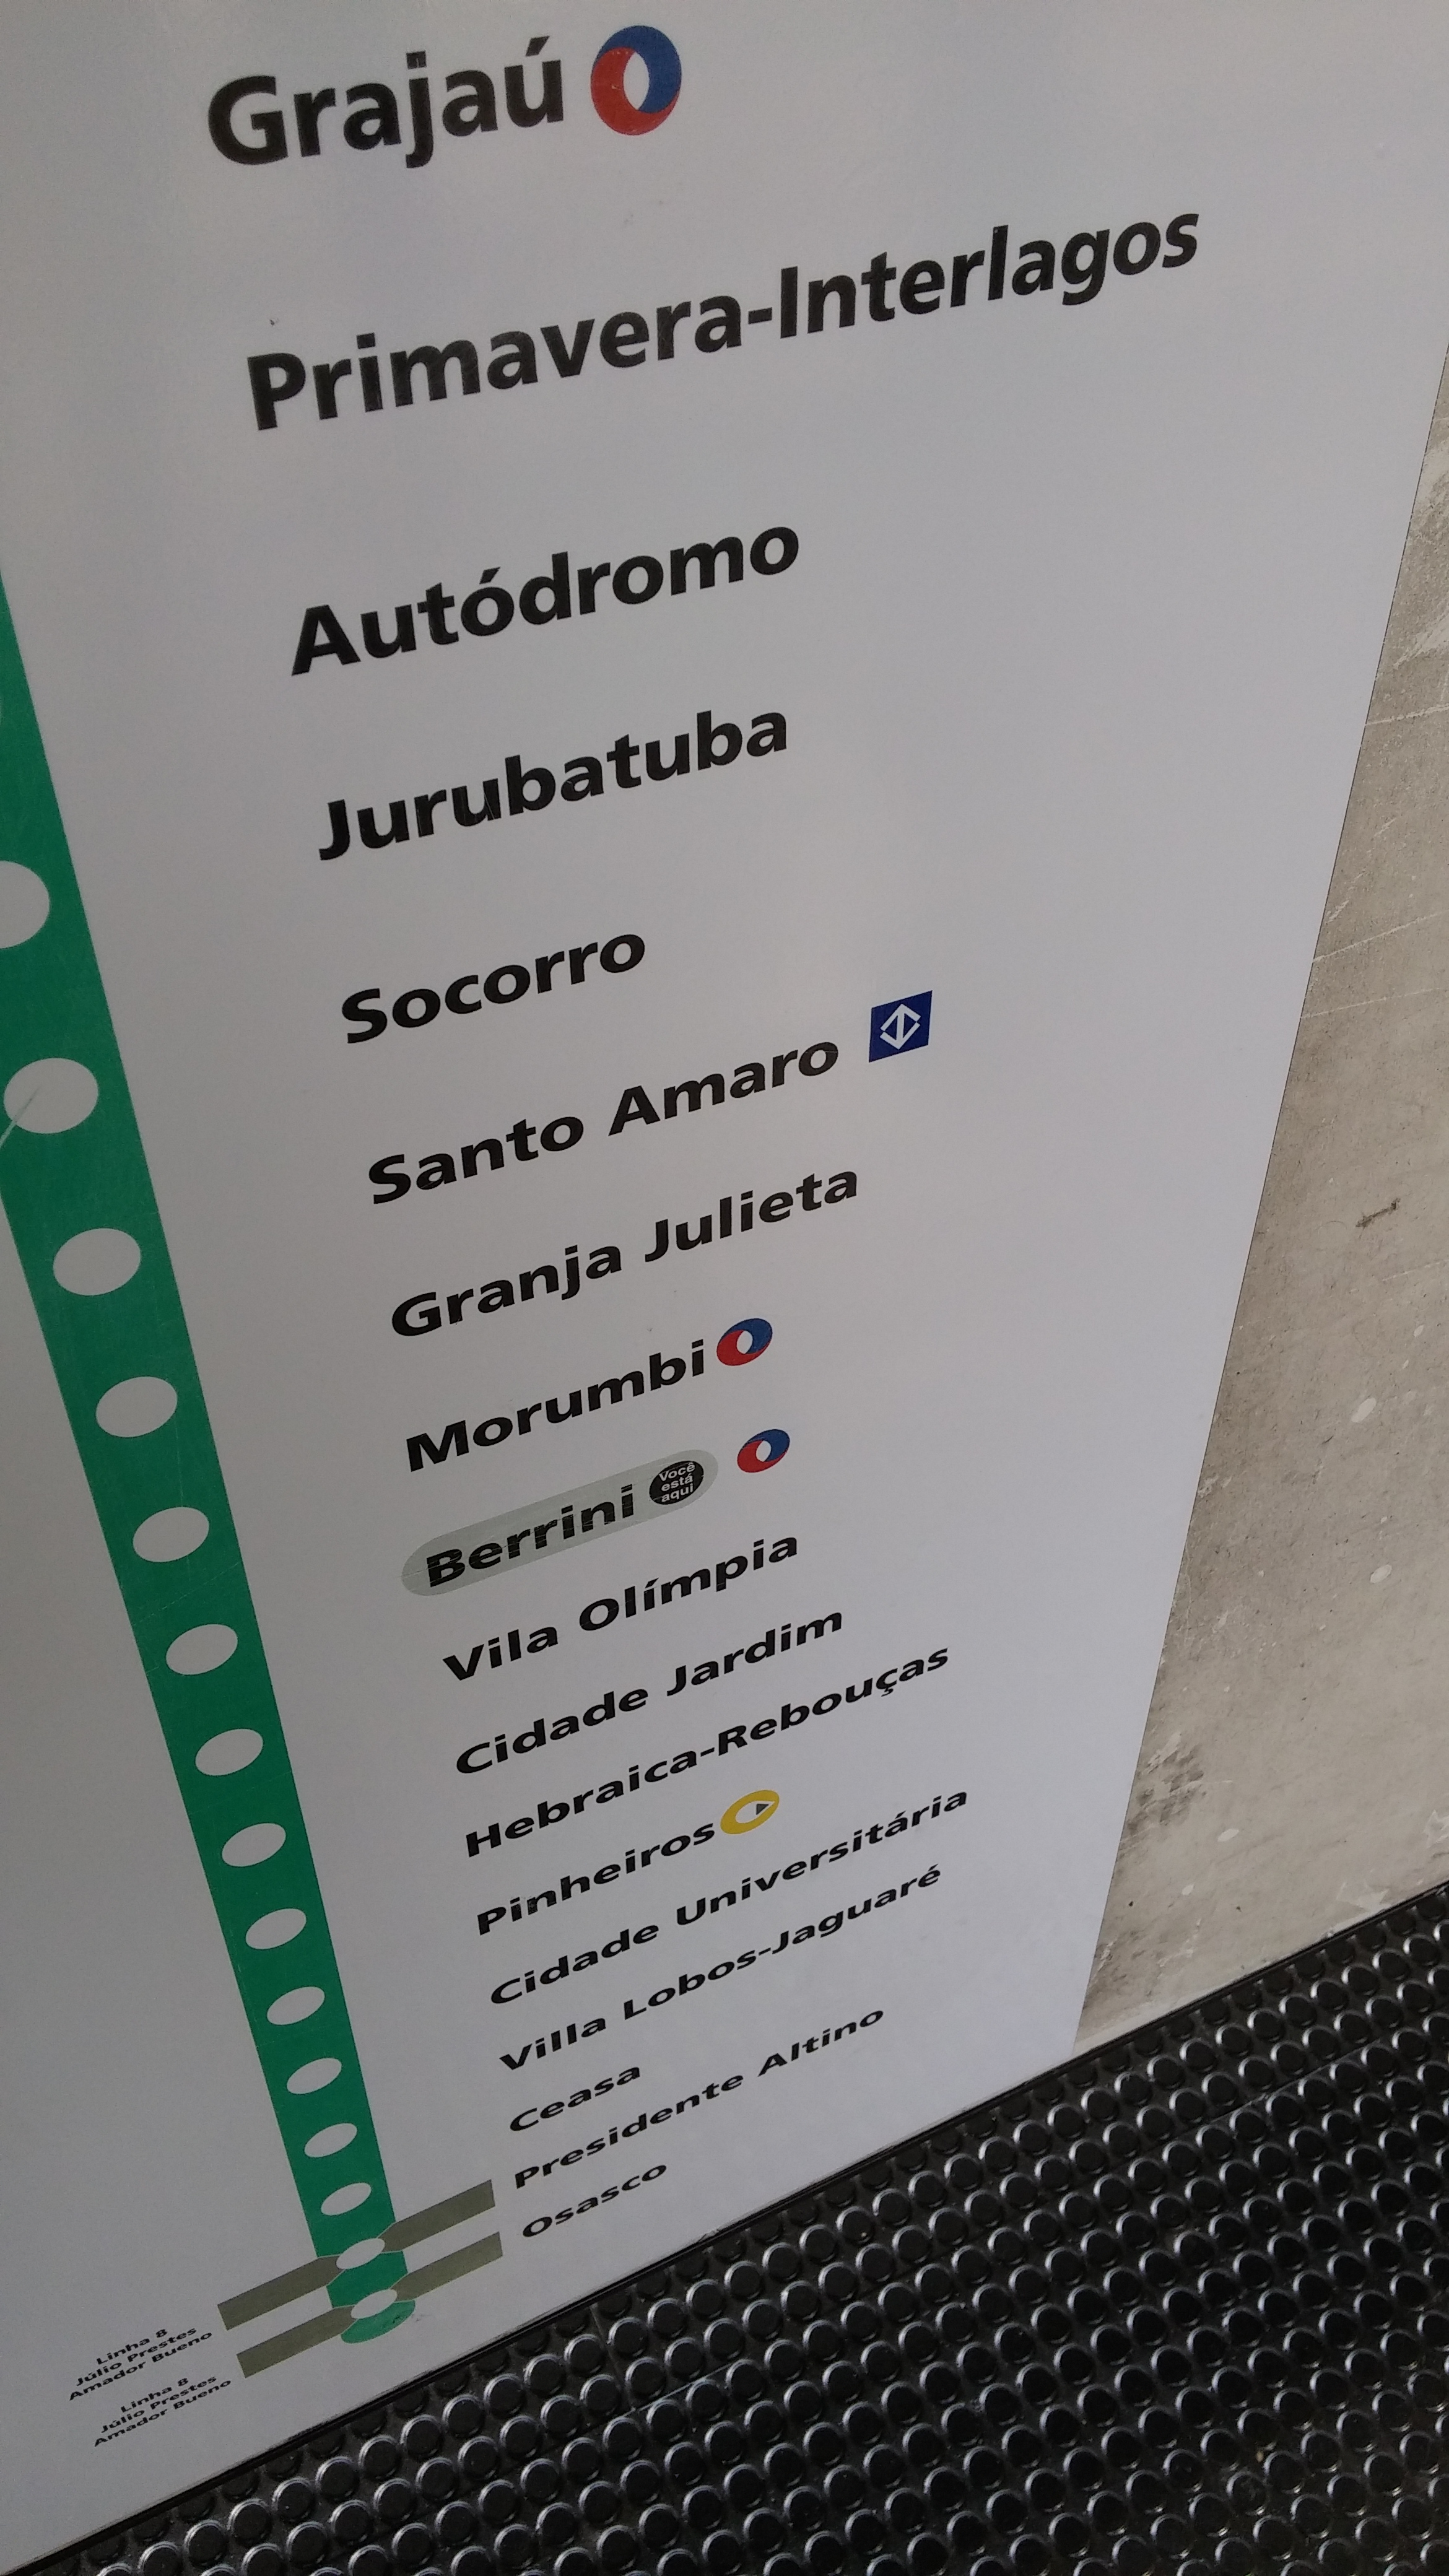
\includegraphics[width=0.9\linewidth]{20160128_170648.jpg}
\end{wrapfigure}

\cite[pág. 13]{Ferreira} explica que a partir dos anos 1970 o setor industrial localizado no centro metropolitano perdeu importância, de forma que o setor terciário, muito menos concentrado e homogêneo no território, absorveu sua mão de obra, o que se traduz em menor polarização, novas localizações (o autor cita shoppings centers e centros empresariais, por exemplo) e alterações significativas no uso do solo \cite[pág. 25]{Ferreira}, o que pode ser relacionado com o processo de rentismo urbano sublinhado por \cite[pág 30, nota de rodapé 2]{Acselrad}, no qual ocorre gentrificação estratégica de áreas urbanas outrora industrializadas e marcadas pelo desinvestimento. A gentrificação se dá a partir das possibilidades econômicas, tanto para valorização, como para aquisição de propriedades imobiliária, num processo que exclui moradores de menor renda \cite[pág. 28-29]{Acselrad}. O trecho central da Linha 9-Esmeralda, que avança ao longo da Avenida das Nações Unidas por regiões enobrecidas e substancialmente modificadas pelo processo, é emblemático, não pode por se encaixar no fenômeno que acaba de ser descrito, como também pela extensão do território afetado, que pode ser observado utilizando as estações da \gls{cptm} como referência, visto que não há, exceto pela Linha 4-Amarela da \gls{cmsp} em regime de concessão patrocinada, outra infraestrutura de transporte de alta capacidade. As estações são: Hebraica\textperiodcentered Rebouças, Cidade Jardim, Vila Olímpia, Berrini e Morumbi.

\begin{landscape}
\begin{figure}[h!]
	\centering
	\caption{Visão dos empreendimentos imobiliários a partir da plataforma da Estação Cidade Jardim (2013} \index{Estação Cidade Jardim}
	\includegraphics[keepaspectratio,width=18.5cm]{DSCN2007.JPG}
\end{figure}
\end{landscape}

\begin{landscape}
\begin{figure}[h!]
	\centering
	\caption{A Estação Cidade Jardim é vizinha de um dos edifícios residenciais mais caros da capital paulista (2013). Fonte: \cite{apecaro}} \index{Estação Cidade Jardim}
	\includegraphics[keepaspectratio,width=18.5cm]{DSCN2000.JPG}
\end{figure}
\end{landscape}

\cite[pág. 201]{Frugoli} destaca a pressão e o desejo de um ator ligado à iniciativa privada com relação à Linha 9, ainda antes do término de sua dinamização, que resultou, sobretudo, na construção e inauguração das estações Hebraica-Rebouças, Cidade Jardim, Berrini, Morumbi, Granja Julieta, Socorro e Vila Olímpia\cite[pág. 38]{Ferreira}: ``"\textemdash\ A linha de metrô está pronta. Está aí no Rio Pinheiros, a linha de trem. Não sei por que, até agora, as nossas "autoridades"\dots Eu acho que os caras não têm visão nenhuma, é uma coisa impressionante. É só fazer algumas estações e está pronta. Não, eles vão fazer, mas só quando fizerem a da Rebouças. Faz já! (Entrevista com Carlos Bratke, cit.)''.

Carlos Bratke, como explica \cite{Frugoli}. exibe perfeitamente os efeitos descritos por \cite{Acselrad}. criticando o poder público, ao mesmo tempo que também demonstra que não era incomodado pela prefeitura ou pelo governo estadual, atuando livremente na Avenida Engenheiro Luís Carlos Berrini:

\begin{citacao}
	As declarações dos irmãos Bratke e matérias da grande imprensa ao longo das últimas décadas ajudam a tecer um quadro que frisa um caráter de "pioneirismo" e "autonomia" quanto ao poder público:
	
	\begin{citacao}
		No espaço de dez anos, [Carlos Bratke, Roberto Bratke e Francisco Collet] operaram em volta da Avenida Luiz Carlos Berrini, sem a mais remota interferência da prefeitura ou de qualquer poder público, uma pequena revolução urbana \textemdash\ a mais notável já feita num grande espaço da cidade por um único projeto privado de arquitetura. (Veja SP, 1985:16)
	\end{citacao}
	
	Na mesma matéria, Carlos Bratke afirma: "Nunca fui procurado por nenhum órgão público para saber quais são os meus planos" (Veja SP, 1985:21).
	
	\begin{citacao}		
		"Essa avenida não é um planejamento urbano. Precisavam fazer um canal, então fizeram essa avenida que ligava nada a coisa nenhuma [\dots] Nessa avenida era tudo abandonado, um brejo. Saímos de pastinha na mão, visitando os amigos e convencendo-os a aplicarem o dinheiro no nosso projeto. Falamos com mais de 200 pessoas e tomei muito chá de cadeira que conseguimos construir o primeiro prédio comercial. Arborizamos a região e valorizamos o metro quadrado de 200 para 5 mil dólares. Já fizemos 30. Estamos fazendo mais trinta. (apud Gabaglia, 1990:s.p.)
	\end{citacao}
	
	Outras críticas ao poder público foram coletadas na entrevista que concedeu:
	
	\begin{citacao}
		\textemdash\ Eu acho que a cidade de São Paulo está constituindo espontaneamente o que os administradores já deviam ter feito há muito tempo: dividir a cidade em vários pólos! [\dots] O zoneamento aqui[região da Berrini] é a coisa mais absurda, anacrônica e idiota que pode existir, mas está acontecendo praticamente numa outra regulamentação. Infelizmente, porque o zoneamento, que já nasceu errado, acabou indo parar nas mãos dos vereadores e não de uma comissão técnica de revisão, nunca foi revisto de uma maneira global, e tem sido alterado ao sabor dos interesses "políticos" dos vereadores. (Entrevista com Carlos Bratke, cit.)
	\end{citacao}	
\end{citacao}

\begin{figure}[h]
	\caption{Visão dos empreendimentos imobiliários a partir da plataforma da Estação Berrini (2016)}
	\includegraphics[keepaspectratio,width=\textwidth]{20160128_170544_HDR.jpg}
\end{figure}

O Trem Metropolitano, no caso da Linha 9-Esmeralda é interessante por dialogar tanto com a Berrini, como outras avenidas similares (em termos de ocupação do solo), como a Chucri Zaidan (Estação Morumbi) ou ainda, conjuntos de ruas e avenidas, como Funchal, Olimpíadas e Dr. Cardoso de Melo (Estação Vila Olímpia), as sete estações do miolo da Linha 9-Esmeralda, todas já mencionadas anteriormente, foram projetadas por Luiz Carlos Esteves, a respeito delas, destaco numa notícia de 22 de junho de 1998 os seguintes fragmentos:

\begin{citacao}
	Até o final de setembro, a população que freqüenta alguns dos edifícios comerciais mais modernos da cidade, situados na avenida das Nações Unidas, zona sul paulistana, vai passar a contar com uma opção de transporte coletivo. Trata-se das sete novas estações de trem que a \gls{cptm} (Companhia Paulista de Trens Metropolitanos) está instalando entre as estações Pinheiros e Largo 13, pertencentes à linha C, que liga Osasco a Jurubatuba.
	
	[\dots]
	
	Luiz Esteves, arquiteto da Harza Hidrobrasileira Engenharia e Projetos, empresa responsável pela concepção e projetos de dinamização da linha Sul, aponta a segurança do usuário como um dos pontos de maior importância das novas estações. “Colocamos a área de bilheteria e catracas junto da calçada dos prédios. Dessa forma, a passarela que leva à plataforma de embarque, do outro lado da marginal, se torna uma área pagante, o que inibe a ação de delinqüentes”, explica.
	
	Outro fator que norteou o projeto, segundo Esteves, foi o urbanismo da região. “Evitamos interferir com o landscape da avenida, projetando estruturas leves e transparentes.” Componentes metálicos fechados com vidro e brises de alumínio garantiram a leveza necessária. O concreto aparece apenas em alguns momentos da estrutura, como a caixa onde serão instaladas duas escadas rolantes, uma escada fixa e um elevador para deficientes. A passarela sobre a marginal também será construída em metal, na forma de uma elipse.
	(\cite{trembom})
\end{citacao}

Na altura, o investimento mencionado foi de US\$ 220 milhões, além disso, Esteves também deu detalhes das estações, então uma novidade. Por se tratar de uma notícia produzida por um periódico especializado em arquitetura, é interessante observarmos que os edifícios da região são enaltecidos ainda antes de introduzir detalhes do investimento feito pelo poder público, a partir daí, vale mencionar que, conforme \cite{Nobre}:

Conforme \cite[pág. 145]{Nobre} a ``associação de promotores imobiliários e investidores corporativos, principalmente os fundos de pensão, permitiu a captação de excedentes de capitais e de poupança que puderam ser desviados para a promoção imobiliária dos megaempreendimentos, criando um grande crescimento desse setor do mercado.''\cite{Nobre}, sendo ainda explicado que a maioria dos empreendimentos ficaram concentrados no Setor Sudoeste da capital paulista em função da estrutura urbana segregada da cidade.

\subsection{Alguns dados}

Conforme dados do \cite{ibgeXSP}, São Paulo tem uma população de 11.253.503 habitantes e possui um território com 1.521.110 km$^2$, atendido por 46 estações\cite{sitecptm1}, das quais 5 foram tratadas aqui (10,9\% do total de estações da \gls{cptm} no município), ainda que de forma mais indireta, principalmente em comparação com a subseção sobre a Linha 8-Diamante.

\begin{center}
	\begin{longtable}{|l|l|l|l|l|l|}
		\caption{Demanda do grupo de estações da Linha 9\, baseado em Mídia \gls{cptm}}\\
		\hline
		\textbf{Média} & \textbf{Hebraica\textperiodcentered Rebouças} & \textbf{Cidade Jardim} & \textbf{Vila Olímpia} & \textbf{Berrini} & \textbf{Morumbi} \\
		\hline
		\endfirsthead
		\multicolumn{6}{c}%
		{\tablename\ \thetable\ -- \textit{Continuado da página anterior}} \\
		\hline
		\textbf{Média} & \textbf{Mooca} & \textbf{Ipiranga} & \textbf{Tamanduateí} \\
		\hline
		\endhead
		\hline \multicolumn{6}{r}{\textit{Continua na próxima página}} \\
		\endfoot
		\hline
		\endlastfoot
		2011 & 18.564 & 16.871 & 25.963 & 20.225 & 20.691 \\
		2012 & 16.363 & 16.891 & 31.733 & 22.893 & 23.105 \\
		2013 & 16.340 & 16.599 & 30.718 & 25.133 & 26.369 \\
		2014 & 16.507 & 15.639 & 32.192 & 25.361 & 28.463 \\
		2015 & 15.872 & 14.820 & 31.130 & 24.238 & 28.048 \\
	\end{longtable}
\end{center}

\begin{center}
	\begin{tikzpicture}
	\begin{axis}[
	title=,
	grid=both,
	ymin=10000,
	ymax=35000,
	scaled ticks=false, tick label style={/pgf/number format/fixed},
	x tick label style={/pgf/number format/1000 sep=},
	y tick label style={/pgf/number format/.cd, set thousands separator={.}},
	legend style={at={(0.5,-0.3)},anchor=north,legend columns=-1},
	ylabel=Passageiros (MDU em milhares),
	xlabel=Ano,
	]
	\addplot coordinates
	{(2011,18564) (2012,16363) (2013,16340) (2014,16508) (2015,15873)};
	\addlegendentry{Hebraica-Rebouças}
	
	\addplot coordinates
	{(2011,16871) (2012,16892) (2013,16599) (2014,15640) (2015,14820)};
	\addlegendentry{Cidade Jardim}	
	
	\addplot coordinates
	{(2011,24327) (2012,25428) (2013,28169) (2014,28347) (2015,23545)};
	\addlegendentry{Vila Olímpia}
	
	\addplot coordinates
	{(2011,18968) (2012,19920) (2013,21281) (2014,21911) (2015,19048)};
	\addlegendentry{Berrini}
	
	\addplot coordinates
	{(2011,18918) (2012,20220) (2013,21527) (2014,22096) (2015,20696)};
	\addlegendentry{Morumbi}
	
	\end{axis}
	\end{tikzpicture}
\end{center}

\begin{obs}
	Seção fortemente baseada em um trabalho de graduação de uma disciplina da Universidade Federal do ABC.
\end{obs}

\begin{info}
	\infocaio{25/04/2016}{https://github.com/caiocco/ufabc-BH0301}
\end{info}

%----------------------------------------------------------------------------------------
% 	PARTE 3
%----------------------------------------------------------------------------------------

\part{Referências}

%----------------------------------------------------------------------------------------
% 	BIBLIOGRAFIA
%----------------------------------------------------------------------------------------

\cleardoublepage
\phantomsection
\chapterimage{2019-02-09_tat_plataforma_l12} % Imagem do cabeçalho do capítulo
%\chapter*{Bibliografia}
\addcontentsline{toc}{chapter}{\textcolor{red}{Bibliografia}}
%\section*{Livros}
%\addcontentsline{toc}{section}{Livros}
%\printbibliography[heading=bibempty,type=Book]
\printbibliography

%----------------------------------------------------------------------------------------
% 	ÍNDICE
%----------------------------------------------------------------------------------------

\cleardoublepage
\phantomsection
\setlength{\columnsep}{0.75cm}
\chapterimage{2018-04-06_psa_arte_l10} % Imagem do cabeçalho do capítulo
\addcontentsline{toc}{chapter}{\textcolor{red}{Índice Remissivo}}
\sffamily
\printindex

%----------------------------------------------------------------------------------------
% 	GLOSSÁRIO
%----------------------------------------------------------------------------------------

\renewcommand{\glossaryname}{Glossário}
%\renewcommand{\glossarypreamble}{Esta é a descrição do glossário.\\ \\}
\renewcommand*{\glsseeformat}[3][\seename]{\textit{#1}
	\glsseelist{#2}}
	
\cleardoublepage
\phantomsection
\setlength{\columnsep}{0.75cm}
\chapterimage{2016-11-04_interior_8500_l11} % Imagem do cabeçalho do capítulo
\addcontentsline{toc}{chapter}{\textcolor{red}{\glossaryname}}
\sffamily
%\glossarystyle{index}
%\glossarystyle{altlisthypergroup}
\glossarystyle{tree}
\printglossaries

%----------------------------------------------------------------------------------------

\end{document}
